%%

\documentclass[phd, print]{nuthesis}
%% Needed to typset the math in this sample
\usepackage{amsmath}
\usepackage{amsfonts}
\usepackage{bm}

%% Let's use a different font
\usepackage[sc,osf]{mathpazo}
\usepackage[T1]{fontenc}
\usepackage[utf8]{inputenc}
\usepackage{mathptmx}

%% superscript and subscript
\usepackage{fixltx2e}

%% To support chemical formula e.g. \ce{SO2}
\usepackage[version=3]{mhchem}

%% Support to fix table width
\usepackage{array}
\newcolumntype{C}[1]{>{\centering\arraybackslash}m{#1}}
\newcolumntype{R}[1]{>{\raggedleft\arraybackslash}m{#1}}

% Heading font size
\usepackage{titlesec}
\titleformat{\chapter} % command
	[display] % shape
	{\normalfont\bfseries \centering \vspace{-2ex}} % format
	{\normalfont\large\MakeUppercase{\chaptertitlename} 
     \MakeUppercase{\thechapter} }
	{0.5em}{\large \centering \MakeUppercase}

%% Makes things look better
\usepackage{microtype}
%\usepackage{indentfirst}

%% Makes things look better
\usepackage{booktabs}

%% Gives us extra list environments
\usepackage{paralist}

%% Be able to include graphicsx
\usepackage{graphicx}

%% For spacing
\usepackage{setspace}

%% Natbib for reference
\usepackage[square]{natbib}
\renewcommand{\bibname}{References}

%% I like darker colors
\usepackage{color}
\definecolor{dark-red}{rgb}{0.6,0,0}
\definecolor{dark-green}{rgb}{0,0.6,0}
\definecolor{dark-blue}{rgb}{0,0,0.6}

%% If you use hyperref, you need to load memhfixc *after* it.
%% See the memoir docs for details.
\usepackage[%
pdfauthor={Xiaoguang Xu},
pdftitle={Dissertation},
pdfsubject={Dissertation},
pdfkeywords={LaTeX, Dissertation, University of Nebraska, Xiaoguang Xu},
linkcolor=dark-blue,
pagecolor=dark-green,
citecolor=dark-blue,
urlcolor=dark-red,
colorlinks=true,
backref,
plainpages=false,% This helps to fix the issue with hyperref with page numbering
pdfpagelabels% This helps to fix the issue with hyperref with page numbering
]{hyperref}

%% Needed by memoir to fix things with hyperref
\usepackage{memhfixc}

%% New commands

%% For equations
\newcommand{\bdeps}{\boldsymbol{\epsilon} } 
\newcommand{\bdsa} {\mathbf{S}_\text{a}}
\newcommand{\bdsy} {\mathbf{S}_\text{y}}
\newcommand{\bdxa} {\mathbf{x}_\text{a}}

\begin{document}
%% Start formating the first few special pages
%% frontmatter is needed to set the page numbering correctly
\frontmatter

\title{Retrieval of Aerosol Microphysical Properties from the AERONET
Photo-Polarimetric Measurements}
\author{Xiaoguang Xu}
\adviser{Professor Jun Wang}
\adviserAbstract{Jun Wang}
\major{Earth \& Atmospheric Sciences \\ (Meteorology/Climatology)}
\degreemonth{May}
\degreeyear{2015}
%%
%% For most people the defaults will be correct, so they are commented
%% out. To manually set these, just uncomment and make the needed
%% changes.
%% \college{Your college}
%% \city{Your City}
%%
%% For most people the following can be changed with a class
%% option. To manually set these, just uncomment the following and
%% make the needed changes.
%% \doctype{Thesis or Dissertation}
%% \degree{Your degree}
%% \degreeabbreviation{Your degree abbr.}
%%
%% Now that we know everything we need, we can generate the title page
%% itself.
%%
\maketitle

%% Front matters, including abstract, dedication, acknowledgements etc.
%%% You have a maximum of 350, which includes your title, name, etc.
\begin{abstract}
  Atmospheric aerosols play an important role in earth climate change by
scattering and absorbing solar and terrestrial radiation, and indirectly
through altering the cloud formation, lifetime, and radiative
properties. However, accurate quantification of these effects is in no
small part hindered by our limited knowledge about the particle size
distribution and refractive index, the aerosol microphysical properties
essentially pertain to aerosol optical and cloud-forming properties. The
focus of this thesis is the  characterization of aerosol microphysical
properties from ground-based polarimetric remote sensing. 

The central research goal is to obtain accurate aerosol PSD and
refractive index of both fine and coarse modes from the multi-spectral
and multi-agular direct and diffuse solar radiation measured by the
SunPhotometer of Aerosol Robertic Network (AERONET). We do so by (1)
developing an inversion algorithm for the retrieval of aerosol
refractive indices and particle size distribution from a combined use of
direct and diffuse solar radiation measurements from AERONET, (2)
conducting a sensitivity study and error budgeting exercise to examine
the potential of adding polarization to the radiance-only inversion, and
(3) performing ground-based retrievals using available AERONET
polarimetric measurements. 

The results from theoretical information and error analysis show a
remarkable increase in information by adding additional polarization
and/or radiances into the inversion: an overall increase of 2--5 of DFS
comparing with radiance-only measurements. Correspondingly, smallest
retrieval errors are found in the added-polarization scenario: 2.3\%
(2.9\%) for the fine-mode (coarse-mode) aerosol volume concentration,
1.3\% (3.5\%) for the effective radius, 7.2\% (12\%) for the effective
variance, 0.005 (0.035) for the real part refractive index, and 0.019
(0.068) for the single scattering albedo. These errors represent a
reduction from their counterparts in the radiance-only scenario of 79\%
(57\%), 76\% (49\%), 69\% (52\%), 66\% (46\%), and 49\% (20\%), respectively.
 In real cases, we found that our retrievals are overall consistent with
AERONET operational inversions, but can offer mode-resolved refractive
index and SSA with acceptable accuracy for the aerosol composed by
spherical particles. Along with the retrieval using both radiance and
polarization, we also performed radiance-only retrieval to demonstrate
the improvements by adding polarization in the inversion. Contrast
analysis indicates that with polarization, retrieval error can be
reduced by over 50\% in PSD parameters, 10--30\% in the refractive index,
and 10--40\% in SSA.
\end{abstract}

%% Optional opyrightpage
%\begin{copyrightpage}
%This file may be distributed and/or modified under the conditions of
%the \LaTeX{} Project Public License, either version 1.3c of this license
%or (at your option) any later version.  The latest version of this
%license is in:
%\begin{center}
%   \url{http://www.latex-project.org/lppl.txt}
%\end{center}
%and version 1.3c or later is part of all distributions of \LaTeX version
%2006/05/20 or later.
%\end{copyrightpage}

%%%%% Optional
%\begin{dedication}
%\begin{center}
%  \vskip.6in
%  To the memory of my grandfather \\
%  \vskip0.2in
%\begin{figure}[h]
%  \centering
%  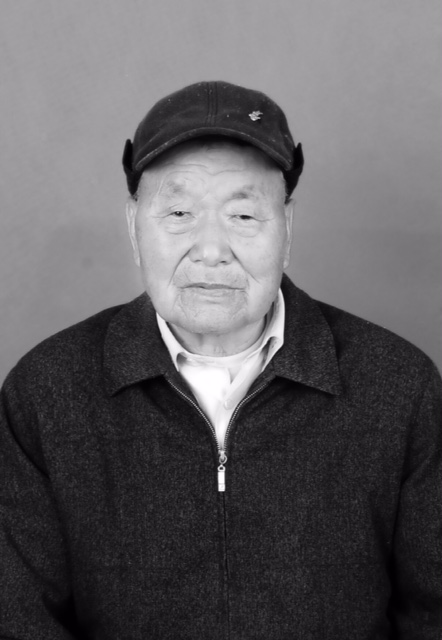
\includegraphics[width={0.35\textwidth}]{figures/grandpapa.jpg}
%  \caption*{\textbf{Zhaoxiang Xu} \\
%(1933 -- 2014)}
%\end{figure}
%\end{center}
%\end{dedication}

%% Optional
\begin{acknowledgments}
  Acknowledgment to be filled \ldots
\end{acknowledgments}

%% Optional
\begin{grantinfo}
  The NASA Earth and Space Science Fellowship funded this project from September
  2012 to August 2015. I am also grateful to the support
  from NASA's New Investigator Program and Radiation Science Program
  (to Dr. Jun Wang).
\end{grantinfo}


%% The ToC is required
%% Uncomment these if need be

%% The ToC is required
\tableofcontents*
%% Uncomment these if need be
\begin{onehalfspacing}
\listoffigures
\listoftables
\end{onehalfspacing}

%% mainmatter is needed after the ToC, (LoF, and LoT) to set the
%% page numbering correctly for the main body
\mainmatter

%% Thesis goes here

% Chapters
%%
\chapter{Introduction}

\section{Background and Motivation}

Atmospheric aerosols play a crucial role in the global climate change. They
affect earth energy budget directly by scattering and absorbing solar and
terrestrial radiation, and indirectly through altering the cloud formation,
lifetime, and radiative properties \citep{haywood00,ramanathan01}.
However, quantification of these effects in the current climate
models is fraught with uncertainties. The global average of aerosol effective
radiative forcing were estimated to range from --0.1 to --1.9 Wm$^{-2}$ with the 
best estimate of --0.9 Wm$^{-2}$ \citep{boucher13}, indicating that the cooling
effects of aerosol might counteract the warming effects of 1.82$\pm$0.19 Wm$^{-2}$
caused by the increase of carbon dioxide since the industrial revolution 
\citep{myhre13}. The climate effects of aerosol particles depend on their
geographical distribution, optical properties, and efficiency as cloud
condensation nuclei and ice nuclei. 
Key quantities pertain to the aerosol optical and
cloud-forming properties include particle size distribution (PSD), chemical
composition, mixing state, and morphology [Boucher et al., 2013]. While the
daily aerosol optical depth (AOD) can be well measured from current satellite
and ground-based remote sensing instrumentations \citep[e.g.,][]{holben98,kaufman02},
the accurate quantification of aerosol ERF is in no
small part hindered by our limited knowledge about the aerosol PSD and
refractive index (describing chemical composition and mixing state). 

To fully understand the role of aerosol particles in the global climate change, 
further development in observations along with retrieval algorithms for these
aerosol microphysical properties from different platforms are thus highly
needed \citep{Mishchenko04}, and the focus of this two-part series study
is the characterization of aerosol properties from ground-based passive remote
sensing.

\subsection{Previous studies on aerosol microphysical retrievals}

There have been continuous efforts in determining aerosol microphysical
properties from ground-based measurements of direct and/or diffuse solar
radiation since \citet{angstrom29} first suggested an empirical relationship
between the spectral dependency of extinction coefficients and the size of
aerosol particles. Over thirty years later, \citet{curcio61} inferred the aerosol
PSD from the spectral particulate extinction coefficients in the visible and
near-infrared regions. Soon with the effective numerical inversion technique
developed by \citet{Phillips62} and \citet{twomey63} specifically for error-involved
optimization, a number of studies explored the use of either spectral
attenuations or scattered radiances (in a small range of scattering angles) to
determine the aerosol PSD
\citep{Twomey67,Yamamoto69,Dave71,Grassl71,Herman71,King78}.
\citet{Shaw79} and \citet{Nakajima83} were among the first studies that have combined
optical scattering measurements with spectral extinctions to recover particle
size spectrum. \citet{Kaufman94} suggested useful information contained in
the sky radiances of larger scattering angles to retrieve the aerosol
scattering phase function and PSD. The first operational retrieval algorithm
for aerosol microphysical properties was introduced by Nakajima et al. [1996],
when the multi-band automatic sun- and sky-scanning radiometer was deployed in
the AErosol RObotic NETwork, or the AERONET [Holben et al., 1994, 1998]. All of
above mentioned methods treated aerosol particles as homogeneous spheres and
with refractive index assumed a priori, even though the refractive index can
highly impact the optical, especially the scattering characteristics [Hansen
and Travis, 1974].  Tanaka et al. [1982, 1983] developed an inversion library
method to estimate the complex refractive index and PSD simultaneously from
measurements of scattered radiances polarized in the perpendicular and parallel
directions. Another concept for determining refractive index from both direct
and diffuse angular radiances was developed by Wendisch and von Hoyningen-Huene
[1994] and Yamasoe et al. [1998], which were based on the fact that
sensitivities of scattered radiances to the PSD and those to the refractive
index are dominated on different scattering-angular regions. The current
AERONET operational inversion algorithm was developed by Dubovik and King
[2000], which has heritage from algorithms developed by King et al. [1978] and
Nakajima et al. [1983, 1996] but was implemented for simultaneous retrieval of
particle size distribution and complex refractive index with sophisticated
inclusion of multiple a priori constraints. Dubovik et al. [2002, 2006] further
implemented the spheroids in the particle shape consideration for desert dust
in the retrieval, and added fractional volume of non-spherical particles to the
inversion products.


\subsection{The AERONET measurements}

\subsection{Challenges and opportunities}

\section{Objectives}

\section{Organization}
 
%%
\chapter{Model Developments} \label{ch:model}

\section{Introduction}

The radiation fields---radiance and the state of polarization---measured by the
AERONET SunPhotometer are the outcome of solar radiation interacting
with various physical processes including the absorption and
scattering by atmospheric molecules, aerosols and clouds, as well the
reflection and absorption by underlying surface. 
The radiance and polarization of light at any wavelength can be represented by
a Stokes column vector $\mathbf{I}$ having four elements \citep{Hansen74}:
\begin{equation}
\mathbf{I} = [I,Q,U,V]^T,
\end{equation}
where $I$ is the total intensity (or radiance), $Q$ and $U$ describe the state of
linear polarization, $V$ describes the state of circular polarization, and $T$
indicates a transposed matrix. It should be noted that all radiation fields and
optical parameters used in this paper are functions of the light wavelength
$\lambda$. For simplicity, however, we omit $\lambda$ in all formulas. 
The degree of linear polarization ($\dolp$) is defined by
\begin{equation}
\dolp = \frac{\sqrt{Q^2+U^2}}{I}. \label{eq:dolp}
\end{equation}

In the solar principal plane, $U$ is negligibly small and the above formula
becomes $\dolp=-Q/I$. Let $\mathbf{I}_0=[I_0,0,0,0]^T$ denote the Stokes vector 
for incident Solar radiation at the top of the atmosphere (TOA) from 
the direction ($\theta_0$, $\phi_0$), where $\theta_0$ and $\phi_0$
are the incident solar zenith and azimuth angles, respectively.
For a plane-parallel atmosphere bounded below by a reflective surface, the
vector radiative transfer equation in the medium for the specific intensity
column vector $\mathbf{I}$ of light propagating in the viewing direction 
($\theta$, $\phi$) can be written \citep{Hovenier04, Mishchenko02}:
\begin{align}
\mu \frac{\partial \mathbf{I}(\tau,\mu,\phi)}{\partial \tau} &=
    \mathbf{I}(\tau,\mu,\phi) - \mathbf{J}(\tau,\mu,\phi; \mu_0, \phi_0)
    \label{eq:rte} \\
\begin{split}
\mathbf{J}(\tau,\mu,\phi; \mu_0, \phi_0) &= 
     \frac{\omega}{4\pi}\int_{-1}^{1}\int_{0}^{2\pi} 
     \mathbf{P}(\tau,\mu,\mu_0,\phi-\phi_0) 
     \mathbf{I}(\tau,\mu_0,\phi_0)\text{d}\phi_0\text{d}\mu_0  \\
     & + \frac{\omega}{4\pi}\mathbf{P}(\tau,\mu,\mu_0,\phi-\phi_0)
     \mathbf{I}_0 \exp(-\tau/\mu_0)
\end{split}
\end{align}
Here, $\tau$ is the extinction optical depth measured from TOA, $\mu$ and
$\mu_0$ are cosines of $\theta$ and $\theta_0$, respectively, $\omega$ is the
SSA and $\mathbf{P}$ is the phase matrix. The first term in equation
\eqref{eq:rte} represents multiple scattering contributions, while
the second indicates scattered light from the direct solar beam. 

Parameters required to solve the above radiative transfer equation are $\tau$,
$\omega$, and $\mathbf{P}(\Theta)$ for the atmosphere, and the reflectance
matrix $\mathbf{R}_\text{s}(\tau,\mu,\phi; \mu_0, \phi_0)$ of 
the underlying surface. Considering a cloud-free atmosphere, the solar
radiation is attenuated by molecular scattering, gaseous absorption, and
aerosol scattering and absorption. For a given layer, we have
\begin{align}
\tau   &= \taua + \taur + \taug  \label{eq:opt1} \\
\omega &= \frac{\taua\assa + \taur}{\tau} \label{eq:opt2} \\
\mathbf{P}(\Theta) &=\mathbf{P}_\text{A}(\Theta)
                     \frac{\taua\assa}{\taua\assa+\taur} 
                    + \mathbf{P}_\text{R}(\Theta)
                    \frac{\taur}{\taua\assa+\taur} \label{eq:opt3}
\end{align}
where $\taua$, $\taur$, and $\taug$ are optical depth, respectively, by 
aerosol extinction, Rayleigh scattering of air density fluctuations, 
and gaseous absorption. $\assa$ is the SSA of aerosol,  and
$\mathbf{P}_\text{A}(\Theta)$ and $\mathbf{P}_\text{R}(\Theta)$ are, 
respectively, the aerosol and Rayleigh phase matrices as functions of the 
scattering angle $\Theta$. Therefore, the forward modeling development 
thus requires the computation of single scattering properties for aerosols and
air density fluctuations, rigorous treatment for absorption of trace gases, 
accuracte representation of reflectance/polarization by surface, an the
realistic simulation of polarimetric radiative transfer. 

In this regard, we have developed the UNified Linearized Vector
Radiative Transfer Model, or UNL-VRTM, specifically for simulation,
analysis, and inversion of the photo-polarimetric measurements.
Components of the UNL-VRTM are described in section \ref{sec:unlvrtm},
and the model benchmarking and verification are presented in section
\ref{sec:rtmverify}.

\section{The UNL-VRTM} \label{sec:unlvrtm}

As shown in Figure \ref{fig:unlvrtm}, the UNL-VRTM comprises 6
modules; they are 
\begin{enumerate}
\item A module computing Rayleigh scattering (section
\ref{subsec:rayleigh});
\item A module that deal with gaseous absorption (section \ref{subsec:rayleigh});
\item A linearized Mie scattering code (section \ref{subsec:mie});
\item A linearized T-matrix electromagnetic scattering code (section
\ref{subsec:mie});
\item A surface model computing various bidirectional
reflectance/polarization functions (BRDF/BPDF) (section
\ref{subsec:surface});
\item A vector linearized radiative transfer model---VLIDORT (section
\ref{subsec:vlidort}). 
\end{enumerate}
These modules are integrated for the forward calculation of
aerosol single scattering, gas absorption, and vector radiative transfer
hereafter, and thus they together constitute the UNified Linearized
Radiative Transfer Model, UNL-VRTM. 

\begin{figure}[t]
  \centering
  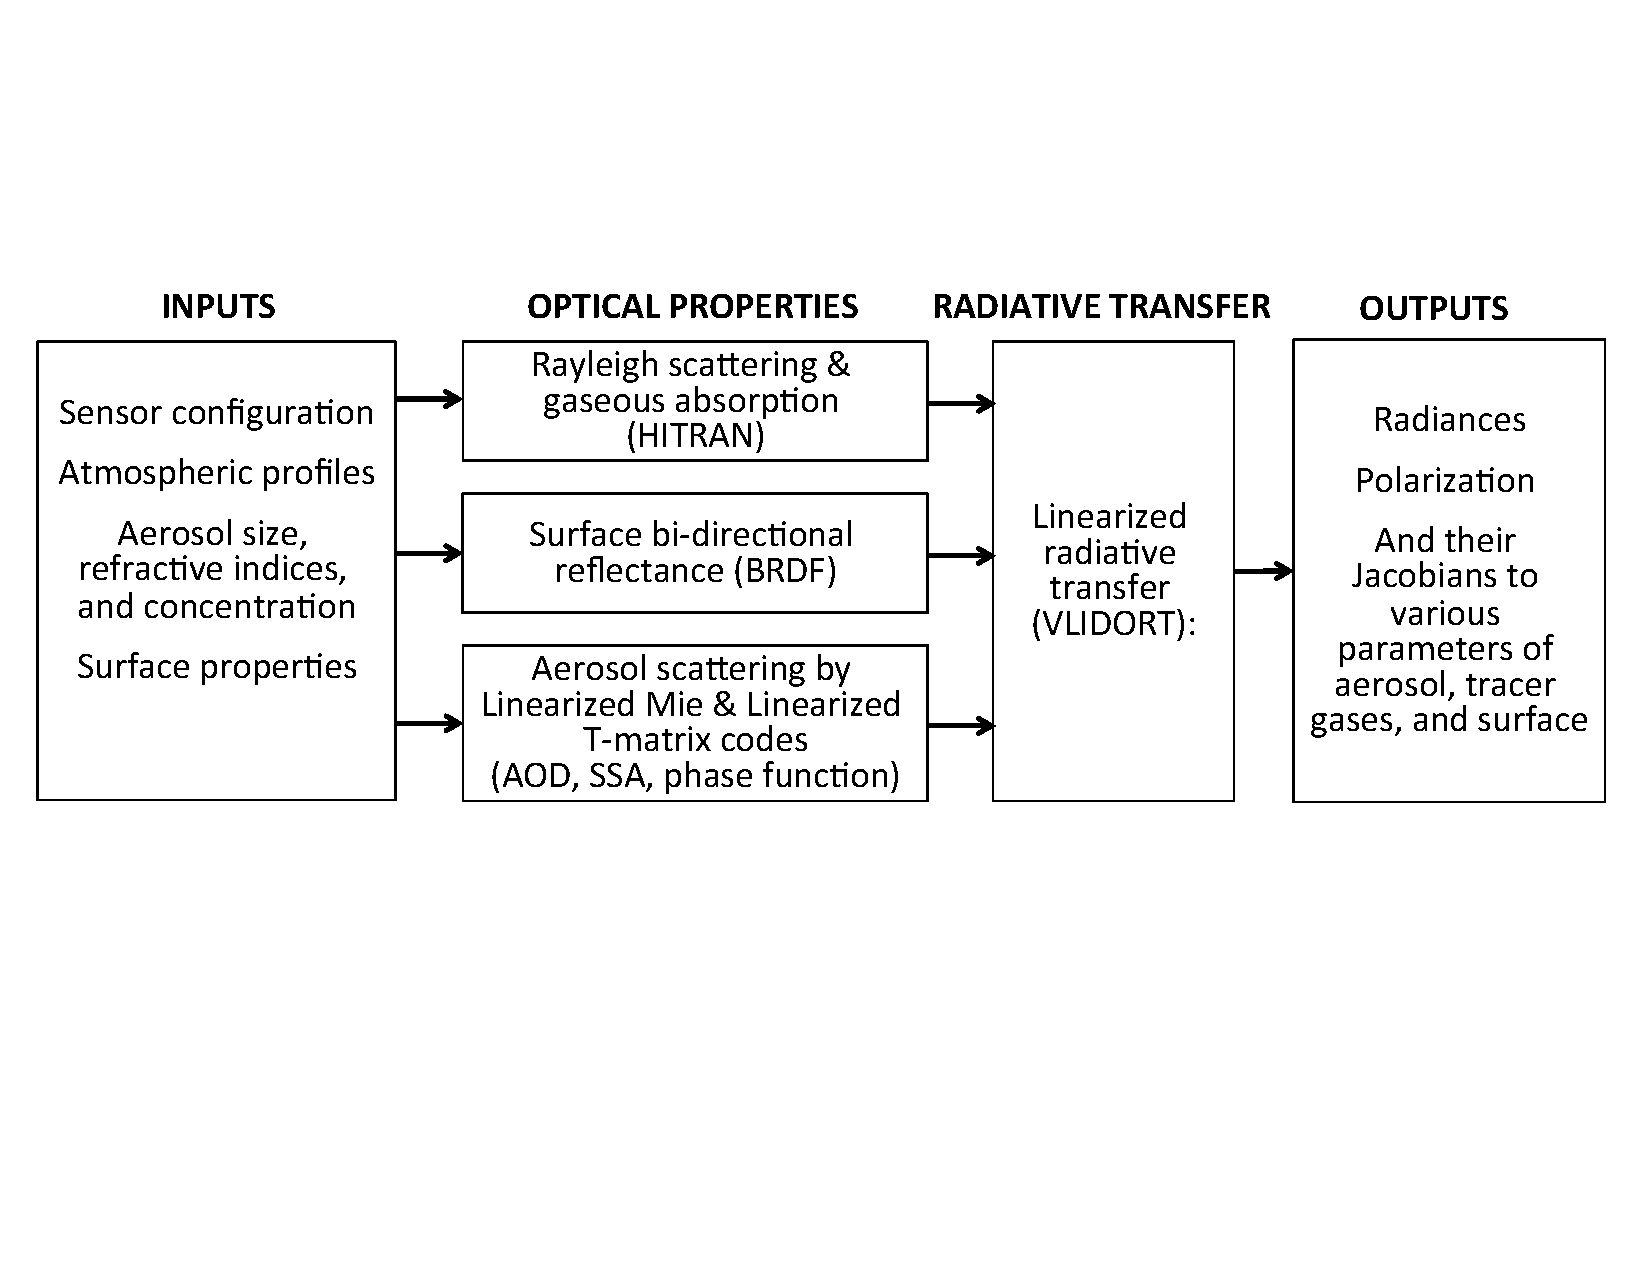
\includegraphics[width={0.95\textwidth}]{figures/unlvrtm.pdf}
  \caption{Flowchart of the UNL-VRTM. See text for detail.}
  \label{fig:unlvrtm}
\end{figure}

Inputs for the UNL-VRTM are profiles of atmospheric properties and
constituents (temperature, pressure, aerosol mass concentration or layer
AOD, water vapor amount and other trace gas volume mixing ratio
profiles \citep{McClatchey72}), the surface properties, as well as 
the aerosol parameters  (such as PSD parameters and refractive index)
themselves. Bearing in mind the lack of
sensitivity in passive remote sensing for the retrieval of vertical
profiles of aerosol properties, the UNL-VRTM as it stands now is only
designed to deliver radiative calculations for a maximum of two sets of
aerosol single scattering properties (e.g., aerosol PSD,
refractive index, and particle shape), typically with one fine-mode and
one coarse-mode aerosol. Other inputs for model include spectral and
geometrical definitions that characterizing specification of an
observing sensor. 

Outputs of the model include the Stokes vector ($\mathbf{I}$) at
user-defined spectral wavelengths and desired atmospheric
levels for both upwelling and downwelling radiation, from which the
light radiance and degree of polarization can be derived. Outputs also
include analytical Jacobians of $\mathbf{I}$ with respect to all aerosol
particle parameters (PSD, refractive index, vertical profile), Rayleigh
scattering optical depth, optical depth of all trace gases, and
parameters describing surface optical property. A detail description of
the UNL-VRTM's Jacobian capability is presented in section
\ref{subsec:jacobian}. 

\subsection{Molecular scattering and absorption} \label{subsec:rayleigh}

The Rayleigh scattering optical depth at certain wavelength in any 
atmospheric layer ($\taur$) is computed by
\begin{equation}
\taur = N_\text{air}\sigma_\text{R} 
\end{equation}
where $N_\text{air}$ is air molecular number density of that layer
(molec cm$^{-2}$), and $\sigma_\text{R}$ is the Rayleigh scattering 
cross-section (cm$^2$ molec$^{-1}$) computed following
\citet{Bodhaine99}. The Rayleigh phase matrix,
$\mathbf{P}_\text{R}(\Theta)$, depends upon molecular 
anisotropy through the depolarization factor, also computed from the same 
source. \citet{Bodhaine99} computes the wavelength-dependent Rayleigh
scattering cross-section as a function of mixing ratios for \ce{N2},
\ce{O2}, \ce{H2O}, and \ce{CO2}. The phase matrix for Rayleigh scattering
follows \citet{Hansen74}; we use the set of spherical-function expansion
 coefficients for the phase matrix as supplied for VLIDORT
\citep{Spurr06}.

Calculation of the absorption optical depth ($\taug$) at
any atmospheric layer for $K$ different trace gases follows
\begin{equation}
\taug = \sum_{i=1}^K N_{\text{gas,}i}\sigma_{\text{A,}i}(T,P) 
\end{equation}
where $N_{\text{gas,}i}$ is the number density of \textit{i}th gas
within that layer, and $\sigma_{\text{A,}i}$ is the corresponding
absorption cross-section, a function of temperature and pressure. 
Our model accounts for absorptions by a total number of
22 trace gases: \ce{H2O}, \ce{CO2}, \ce{O3}, \ce{N2O}, \ce{CO},
\ce{CH4}, \ce{O2}, \ce{NO}, \ce{SO2}, \ce{NO2}, \ce{NH3}, \ce{HNO3},
\ce{OH}, \ce{HF}, \ce{KCl}, \ce{HBr}, \ce{HI}, \ce{ClO}, \ce{OCS},
\ce{H2CO}, \ce{HOCl}, and \ce{N2}.
The determination of $\sigma_\text{A}$  
utilizes a UV-to-visible cross-section library and the line-spectroscopic
absorption parameters archived in the HITRAN database \citep{Orphal03,
Rothman09}. The cross-section library compiles the extinction
cross-section for \ce{O3}, \ce{NO2}, \ce{SO2}, and \ce{O2-O2} in the UV
and/or visible spectral regions. Meanwhile, line-spectroscopic 
absorption databased are used to simulate the pressure- and
temperature-dependent extinction cross-section with line-by-line (LBL) 
approach \citep{Liou02,Rothman09} by accumulating each individual 
absorption line. Doppler broadening is calculated from the molecular mass
and the temperature, and Doppler and Lorentz broadening are included in the
Voigt calculation.

Particular to work, we only consider the most influential 
trace species for the AERONET spectral bands: \ce{H2O} (vapor), \ce{O3}, 
and \ce{NO2}. In our algorithm (section \ref{ch:algorithm}), the columnar
amounts of \ce{O3} and \ce{NO2} are dynamically adjusted with retrievals from the
Ozone Monitoring Instrument (OMI) \citep{Levelt06} on board the
AURA satellite. We apply the columnar water vapor amount retrieved from
the 940-nm radiances measured by the AERONET SunPhotometer
\cite{Halthore97}.

\subsection{Aerosol single scattering} \label{subsec:mie}

Aerosol single scattering properties necessary to the radiative
transfer calculation include aerosol optical depth ($\taua$)
($\qext$), SSA ($\assa$), and scattering phase matrix ($\paer(\Theta)$).
The calculation of these parameters is made with a Linearized Mie (LMIE)
scattering electromagnetic code for spherical particles and a Linearized
T-matrix (LTMATRIX) scattering code for non-spherical convex and axially
symmetric particles \citep{Spurr12}. The LMIE code originates from the Mie code
of \citet{deRooij84}, and the LTMATRIX code originates from the T-Matrix
code developed by \citet{Mishchenko96, Mishchenko98}; both include
linearization capabaility developed by \citet{Spurr12}.

Common inputs for both codes are the complex refractive index
($\mreal + i\mimag$), and the particle size distribution (PSD) 
parameters for polydisperse scattering. The codes have several options 
to specify the PSD function: two-parameter gamma, two-parameter 
lognormal, three-parameter modified gamma, and four-parameter bi-lognormal. 
In addition, the linearized T-matrix code offers options to characterize the 
shape of non-spherical aerosols (spheroids, cylinders, or Chebyshev particles)
\citep{Spurr12}. For non-spherical particles, the specified size distribution 
is interpreted as the equivalent surface-area sphere in the linearized T-matrix
calculation, regardless of the shape. 

For AERONET inversion alorithm, we assume that the aerosol volume
distribution follows a bi-modal lognormal function \citep[in agreement
wit][]{Schuster06, Waquet09}:
\begin{equation}
\frac{\text{d}V}{\text{d}\ln{r}} = \sum_{i=1}^2 
\frac{V_0^i}{\sqrt{2\pi}\ln{\sg^i}} 
\exp{\left[ -\frac{(\ln{r}-\ln{\rv^i})^2}{2\ln^2{\sg^i}}\right]}
\end{equation}
where $V_0$, $\rv$, and $\sg$ are the total volume concentration, geometric
median radius, and standard deviation, respectively. The superscript $i$
indicates the size mode, and later will be replaced by ‘f’ for fine mode
and ‘c’ for coarse mode. We assume that particle size ranges from 0.01
to 10 $\mu$m for the fine mode and from 0.05 to 20 $\mu$m for
the coarse mode, both covering $>$ 99.9\% of the total volume of an 
idealistic size range (0, $+\infty$). An advantage of the lognormal 
distribution is that standard deviations for the number, area, and 
volume PSD functions are identical, and therefore allowing that the 
median radii for these PSD functions can be converted from one to 
another \citep{Seinfeld06}. The $\reff$ and $\veff$ are related to 
the geometric parameters through:
\begin{align}
\reff &= \rv \exp{\left( -\frac{1}{2} \ln^2{\sg}\right)}, \\
\veff & = \exp{\left(\ln^2{\sg}\right)} - 1.
\end{align}

The LMIE/LTMATRIX code computes the aerosol extinction efficiency
factor $\qext$, single scattering albedo $\assa$, and phase matrix 
$\paer(\Theta)$, as well as Jacobians of these quantities with respect
to input parameters including $\reff$, $\veff$, $\mreal$, and $\mimag$.
The phase matrix and its Jacobians are expressed in terms of the
coefficients $\baer(\Theta)$ for each moment $l$ in terms of the 
generalized spherical function expansions
for each non-zero phase matrix element. Let $\mathbf{A}$ denotes the
vector of aerosol microphysical parameters, 
$\mathbf{A}=[V_0,\reff,\veff,\mreal,\mimag]^T$, and $\mathbf{M}$
the vector of aerosol optical parameters, 
$\mathbf{M}=[\taua,\assa,\baer(\Theta)]^T$, 
where $\taua$ is related to $\qext$ by 
$\taua=\frac{3V_0 \qext}{4\reff}$. The LMIE/LTMATRIX code acts
as an operator that maps vector $\mathbf{A}$ to $\mathbf{M}$. 
The Jacobian matrix of $\mathbf{M}$ with respect to $\mathbf{A}$ calculated by 
means of the linearization feature of the code, and it can be expressed by
$\nabla_\mathbf{A}\mathbf{M}$. 

\subsection{Surface representations} \label{subsec:surface}

VLIDORT has a supplementary module for specification of the surface BRDF
as a linear combination of (up to) three semi-empirical kernel
functions; for details, see \citet{Spurr04}. This supplementary module can also
provide partial derivatives of the BRDF with respect to the kernel
weighting factors or with respect to kernel parameters such as the wind
speed for glitter reflectance. These kernel functions include
Lambertian, Ross-Thick, and Li-Sparse functions \citep{Wanner95, Lucht00}, a
Bi-directional Polarization Distribution Function (BPDF)
\citep{Maignan09}, and an ocean surface model based on the 
Cox-Munk model \citep{Cox54}. In addition, VLIDORT has
an option for using a surface-leaving radiation field, either as a
fluorescence term or as a water-leaving term expressed as a function of
chlorophyll absorption.

Although surface reflectance has in general a low influence on AERONET
down-welling sky radiances and polarization, a state-of-the-art
representation of the surface reflectivity potentially reduces model
uncertainties, especially for measurements taken at low elevation angles
that could be affected by surface diffusion. Here, we utilize the
spectral BRDF parameters from the MODIS surface products that are
operationally reported every 16 days at a 1-km resolution
\citep{Lucht00}. Here we use time-matched MODIS BRDF products 
to reconstruct the bidirectional reflectance over AERONET stations.
The MODIS BRDF product supplies three weighting parameters
($f_\text{iso}$, $f_\text{vol}$, and $f_\text{geo}$) for the first 
7 MODIS bands, respectively, corresponding to three kernel types:
isotropic, Ross-Thick ($K_\text{vol}$), and Li-Sparse ($K_\text{geo}$):
\begin{equation}
\rho_\text{R}(\mu,\phi;\mu_0,\phi_0) = f_\text{iso} + 
f_\text{vol}K_\text{vol}(\mu,\phi;\mu_0,\phi_0) +
f_\text{geo}K_\text{geo}(\mu,\phi;\mu_0,\phi_0)  \label{eq:brdf}
\end{equation}
Expanded expressions for $K_\text{vol}$ and $K_\text{geo}$ appear in
\citet{Wanner95, Lucht00}. 

Studies have shown that the BPDF for land surfaces is generally rather
small and is “spectrally neutral” \citep{Nadal99, Maignan04, Maignan09,
Waquet07, Litvinov11}. 
Most empirical BPDF models are based on Fresnel coefficients of light
reflectance from the surface. Here we have incorporated the
one-parameter model developed by \citet{Maignan09}, which was
derived from analyses of several years of POLDER/PARASOL measurements.
This model describes the polarized reflectance at any viewing geometry
($\mu$, $\phi$) from the given incident geometry ($\mu_0$, $\phi_0$) as:
\begin{equation}
\pmb{\rho}_\text{P}(\mu,\phi;\mu_0,\phi_0) = 
\frac{C_0 \exp(-\tan \theta_\text{h})\exp(-\text{NDVI})}{\mu_0+\mu} 
\mathbf{F}_\text{P}(\theta_\text{h},n_\text{v}) \label{eq:bpdf}
\end{equation}
where $C_0$ is a constant parameter chosen for a certain surface type,
$\theta_\text{h}$ is half of the phase angle of reflectance, $n_\text{v}$ is 
the refractive index of vegetation (1.5 is used), and
$\mathbf{F}_\text{P}$ is the Fresnel reflection matrix. 
We chose a spectrally-independent value for $C_0$ based
on the recommendations by \citet{Maignan09} for relevant surface types. 

The combination of the BRDF and BPDF for land surface follows the
discussion by \citet{Dubovik11}. The surface reflectance matrix 
$\mathbf{R}_\text{s}(\mu,\phi;\mu_0,\phi_0)$
is represented as a sum of diffuse unpolarized
reflectance and specular reflectance; the former is modeled using the
MODIS BRDF in equation \eqref{eq:brdf}, and the latter using the BPDF 
formula in equation \eqref{eq:bpdf}. 

\subsection{Radiative transfer} \label{subsec:vlidort}

The radiative transfer equation \eqref{eq:rte} is solved with the 
Vector Linearized Discrete Ordinate Radiative Transfer (VLIDORT)
model, which is a core part of the UNL-VRTM. VLIDORT, 
developed by \citet{Spurr06}, is a
linearized pseudo-spherical vector discrete ordinate radiative transfer
model for multiple scattering of diffuse radiation in a stratified
multi-layer atmosphere. It computes four elements of the Stokes vector I
for downwelling and upwelling radiation at any desired atmospheric
level. The VLIDORT includes the pseudo-spherical approximation to
calculate solar beam attenuation in a curved medium. It also uses the
delta-M approximation for dealing with sharply peaked forward
scattering. Specifically for the AERONET inversion, we consider 16
discrete ordinate streams in the radiative transfer calculation and
retain 180 terms in the spherical-function expansion of the scattering
matrix to ensure accurate calculation of diffuse radiation. 

Along with the Stokes vector $\mathbf{I}$, VLIDORT also computes the Jacobian
matrix of I with respect to aerosol optical vector $\mathbf{M}$, 
$\nabla_\mathbf{M}\mathbf{I}$. Therefore,
the combination of the VLIDORT and the LMIE/LTMATRIX codes allows for a
direct calculation of the Jacobian matrix of the Stokes vector with
respect to aerosol microphysics, $\mathbf{A}$, by
\begin{equation}
\nabla_\mathbf{A}\mathbf{I} = \nabla_\mathbf{M}\mathbf{I}
\cdot \nabla_\mathbf{A}\mathbf{M} \label{eq:adj-i}
\end{equation}
Essentially, the above equation can yield the derivatives of the
radiance $I$ and $\dolp$ with respect to any aerosol microphysical parameter,
i.e., $\nabla_\mathbf{A}I$ and $\nabla_\mathbf{A}\dolp$. 
While obtaining $\nabla_\mathbf{A}I$ is straightforward,
$\nabla_\mathbf{A}\dolp$ can be derived from equation \eqref{eq:dolp} 
following:
\begin{equation}
\nabla_\mathbf{A}\dolp = -\frac{\dolp \nabla_\mathbf{A}}{I} +
\frac{Q\nabla_\mathbf{A}{Q}+U\nabla_\mathbf{A}{U}}{I\sqrt{Q^2+U^2}}
\label{eq:adj-dolp}
\end{equation}

\subsection{Capability of calculating Jacobians} \label{subsec:jacobian}

This section analytically derives the Jacobian of $\mathbf{I}$ with
respect to various aerosol related parameters, including $\taua$,
$\assa$, $\baer$, refractive index, PSD parameters, and aerosol vertical
profile. Computation of the Stokes vector in VLIDORT requires input of
an optical property set $[\tau,\omega,\left<\mathbf{B}^j\right>_{j=0,J}]$ for
each atmospheric layer, where $<>_{j=0,J}$ denotes the vector that
consists of elements having the similar expression as that inside $<>$
but for $j=0, J$. For each atmospheric layer $L$, the optical property
inputs are assumed constant and are given by equations 
\eqref{eq:opt1}--\eqref{eq:opt2}, as well as equation \eqref{eq:opt3}
with $\mathbf{P}(\Theta)$ replaced by $\mathbf{B}^j$. 
It should be noted that all parameters
in these requations are for each layer, but we ignore $L$ for
convenience.

Since VLIDORT generates Jacobians with respect to layer-integrated
single scattering properties in each atmospheric layer as well as
column-integrated single scattering property as a whole, and LMIE and
LTMATRIX offer the sensitivity of aerosol scattering properties to
microphysical aerosol physical parameters, an integrated use of VLIDORT
and LTMATRIX/LMIE can, in principle, provide the Jacobians of Stokes
parameters with respect to both aerosol single scattering properties as
well as aerosol microphysical parameters (as expressed by equations
\eqref{eq:adj-i}--\eqref{eq:adj-dolp}). Practically, the VLIDORT
calculation of Jacobians of any Stokes parameter $\xi$ with respect to 
any aerosol parameter $x$ proceeds according to
\begin{equation}
\begin{split}
x\frac{\ptxi}{\partial x} &=
  x\left[ \frac{\ptxi}{\pttau}, \frac{\ptxi}{\ptssa}, 
          \left< \frac{\ptxi}{\ptb^j}\right>_{j=1,J}\right] 
  \left[ \frac{\pttau}{\ptx}, \frac{\ptssa}{\ptx}, 
         \left< \frac{\ptb^j}{\ptx}\right>_{j=1,J}\right]^T \\
  &= \left[ \tau \frac{\ptxi}{\pttau}, \omega \frac{\ptxi}{\ptssa}, 
          \left< \mathbf{B}^j \frac{\ptxi}{\ptb^j}\right>_{j=1,J}\right]
     \left[ \phi_x, \varphi_x, \left< \pmb{\Psi}_x^j\right>_{j=1,J}
\right]^T. 
\end{split}
\label{eq:adj-x}
\end{equation}

The first square bracket on the right-hand side of equation
\eqref{eq:adj-x} contains quantities computed internally by VLIDORT, 
while the second so-called “transformation vector” must be supplied 
by users and is defined as:
\begin{equation}
\phi_x = \frac{x}{\tau}\frac{\pttau}{\ptx}; \quad 
\varphi_x = \frac{x}{\omega}\frac{\ptssa}{\ptx}; \quad 
\pmb{\Psi}_x^j = \frac{x}{\mathbf{B}^j}\frac{\ptb^j}{\ptx}.
\end{equation}

%% Table 
\begin{table}[t]
  \centering
  \small
  \caption{Elements of transformation vector for various aerosol single
scattering parameters (composite of fine and coarse mode).}
  \label{tab:jacobian1}
  \begin{tabular}{p{2em} p{2em} p{5em} p{15em} }
    \toprule
       $x$ & $\phi_x$ & $ \varphi_x$ & $\pmb{\Psi}_x^j$ \\
    \midrule
    $\taua$        & $\frac{\taua}{\tau}$ &
$\frac{\taua}{\tau}\left( \frac{\assa}{\omega}-1\right)$ &
$\left\{ \begin{array}{ll} \frac{\assa\taua}{\omega\tau}\left(
\frac{\baer^j}{\mathbf{B}^j}-1 \right)
&\mbox{for } j<3  \\ \frac{\taur}{\omega\tau} & \mbox{for } j\geq 3
\end{array} \right.$\\  
    $\assa$        & 0 & $\frac{\taua\assa}{\tau\taua\assa+\taur}$ &
Same as above \\
    $B_\text{A}^j$ & 0 & 0 & $\left\{ \begin{array}{ll}
\frac{\assa\taua\baer^j}{\assa\taua\baer^j+\taur\mathbf{B}_\text{R}^j}
&\mbox{for } m=j<3  \\ 1 & \mbox{for } m=j\geq 3 \\ 0 & \mbox{for }
m\neq j
\end{array} \right.$ \\
    \bottomrule
  \end{tabular}
\end{table}

As we are interested in aerosol parameters, this transformation vector
can be further expanded as 
\begin{equation}
\left[ \phi_x, \varphi_x, \left< \pmb{\Psi}_x^j\right>_{j=1,J}\right]^T
=\pmb{\Pi} \left[ \phi_x^\prime, \varphi_x^\prime, \left<
\pmb{\Psi}_x^{\prime j}\right>_{j=1,J}\right]^T, \label{eq:trans}
\end{equation}
where
\begin{equation}
\phi_x^\prime = \frac{x}{\taua}\frac{\pttaua}{\ptx}, \quad 
\varphi_x^\prime = \frac{x}{\scaa}\frac{\ptscaa}{\ptx}, \quad  \mbox{and} 
\pmb{\Psi}_x^{\prime j} = \frac{x}{\baer^j}\frac{\ptbaer^j}{\ptx},
\end{equation}
and $\pmb{\Pi}$ is a matrix expressed by
\begin{equation}
\pmb{\Pi} = \left[ 
            \begin{array}{lll}
            \frac{1}{\tau}  & \pmb{0} & \pmb{0} \\
            -\frac{1}{\tau} & \frac{1}{\scaa+\taur} & \pmb{0} \\
            \pmb{0} & \left<
\frac{\baer^j-\bray^j}{\mathbf{B}^j(\scaa+\taur)}\right>_{j=1,J} & 
\left< \frac{\scaa}{\mathbf{B}^j(\scaa+\taur)}\right>_{j=1,J}
            \end{array}
            \right]. \label{eq:pi}
\end{equation}
Here, $\scaa$ is the scattering optical depth of aerosols. The detailed
derivations of the matrix $\pmb{\Pi}$ are presented in Appendix \ref{app:pi}. 
Hence, the transformation vector for calculating Stokes profile Jacobians 
with respect to $\taua$, $\assa$, $\baer^j$ can be obtained by combining 
equations \eqref{eq:trans} and \eqref{eq:pi}, and the components of 
this vector are listed in Table \ref{tab:jacobian1}.

In an atmosphere where both fine (superscript “f”) and coarse
(superscript “c”) aerosol particles co-exist, the ensemble aerosol
optical properties may be derived by assuming external mixing:
\begin{equation}
\left\{  
\begin{array}{ll}
\taua &= \taua^\text{f} + \taua^\text{c} \\
\scaa &= \scaa^\text{f} + \scaa^\text{c} \\
\baer^j &= \frac{\scaa^\text{f} + \scaa^\text{c}}
           {\scaa^\text{f}\baer^{\text{f},j} + \scaa^\text{c}\baer^{\text{c},j} }
\end{array} 
\right.
\end{equation}


\begin{table}[t]
  \centering
  \small
  \caption{Elements of transformation vector for various microphysical
parameters of fine and coarse mode aerosols.}
  \label{tab:jacobian2}
  \begin{tabular}{p{4em} p{10em} p{10em} p{11em} }
    \toprule
       $x$ & $\phi_{x\fine}^\prime$ & $\varphi_{x\fine}^\prime$ &
$\pmb{\Psi}_{x\fine}^{\prime j}$ \\
    \midrule
    $\taua\fine$ & $\taua\fine$ & $\scaa\fine$ & 
    $\frac{\scaa\fine}{\taua}(\baer^{\text{f}j}-\baer^j)$ \\
    $\assa$ & 0 & $\scaa\fine$ &
    $\frac{\scaa\fine}{\taua}(\baer^{\text{f}j}-\baer^j)$ \\ 
    $V_0\fine$ & $\frac{3V_0\fine\qext\fine}{4\reff\fine}$ &
    $\frac{3V_0\fine\qsca\fine}{4\reff\fine}$ &
    $\frac{\scaa\fine}{\taua}(\baer^{\text{f}j}-\baer^j)$ \\ 
    $\mreal\fine,\mimag\fine$ & 
    $\taua\fine\frac{x\fine}{\qext\fine}\frac{\partial\qext\fine}{\ptx\fine}$ &
    $\scaa\fine\frac{x\fine}{\qsca\fine}\frac{\partial\qsca\fine}{\ptx\fine}$ & 
    $\frac{\varphi_{x\fine}^\prime}{\scaa\fine}(\baer^{\text{f}j}-\baer^j)+x\fine\frac{\partial\baer^{\text{f}j}}{\ptx\fine}$ \\
    $\rg\fine,\sg\fine,\epsilon\fine$ &
    $\taua\fine(\frac{x\fine}{\qext\fine}\frac{\partial\qext\fine}{\ptx\fine}-\frac{x\fine}{\reff\fine}\frac{\partial\reff\fine}{\ptx\fine})$ & 
    $\scaa\fine(\frac{x\fine}{\qsca\fine}\frac{\partial\qsca\fine}{\ptx\fine}-\frac{x\fine}{\reff\fine}\frac{\partial\reff\fine}{\ptx\fine})$ &
    $\frac{\varphi_{x\fine}^\prime}{\scaa\fine}(\baer^{\text{f}j}-\baer^j)+x\fine\frac{\partial\baer^{\text{f}j}}{\ptx\fine}$ \\
    $H\fine$ & $H\fine\frac{\pttaua}{\partial{H\fine}}$ &
    $\phi_{x\fine}^\prime\assa\fine$ &
    $\frac{\scaa\fine}{\taua}(\baer^{\text{f}j}-\baer^j)$ \\
    \bottomrule
  \end{tabular}
\end{table}

We can generate the transformation vectors (as listed in Table
\ref{tab:jacobian2}) for any of the following parameters: $\taua\fine$, 
$\assa\fine$, $V_0\fine$, $\mreal\fine$, $\mimag\fine$, $\rg\fine$,
$\sg\fine$, $\epsilon\fine$, $H\fine$, and $\taua\coarse$,
$\assa\coarse$, $V_0\coarse$, $\mreal\coarse$, $\mimag\coarse$,
$\rg\coarse$, $\sg\coarse$, $\epsilon\coarse$, and $H\coarse$. Here,
$\rg$, $\sg$, and $H$ denote the median and standard deviation of the
particle radius (e.g., two parameters in the log-normal aerosol number
distribution), and the scale height of aerosol extinction, respectively.
$V_0$ is the aerosol volume concentration and $\epsilon$ the shape 
factor of the non-spherical particle. Details of the algebra for deriving 
the transformation vectors may be found in Appendix \ref{app:pi}. 
Note that the shape of the aerosol extinction vertical profile in the
testbed is assumed to be constant or exponentially decreasing with
height or quasi-Gaussian (Appendix \ref{app:pi}). The analytical
formulas for $\phi_x^\prime$, $\varphi_x^\prime$, and
$\pmb{\Psi}_x^{\prime j}$ for coarse mode aerosol parameters are
the same as their counterparts for fine-mode aerosols; we need only
replace superscript “s” with “c” in Table 3 entries. Jacobians with
respect to the fine mode fraction, either in terms of AOD
($\fmftau$) or in terms of the volume concentration ($\fmfv$), 
can be derived from the corresponding Jacobians with respect to 
modal AOD and volume, respectively:


%%%% New section
\section{Model Benchmarking and Verifications} \label{sec:rtmverify}

\begin{figure}[p]
  \centering
  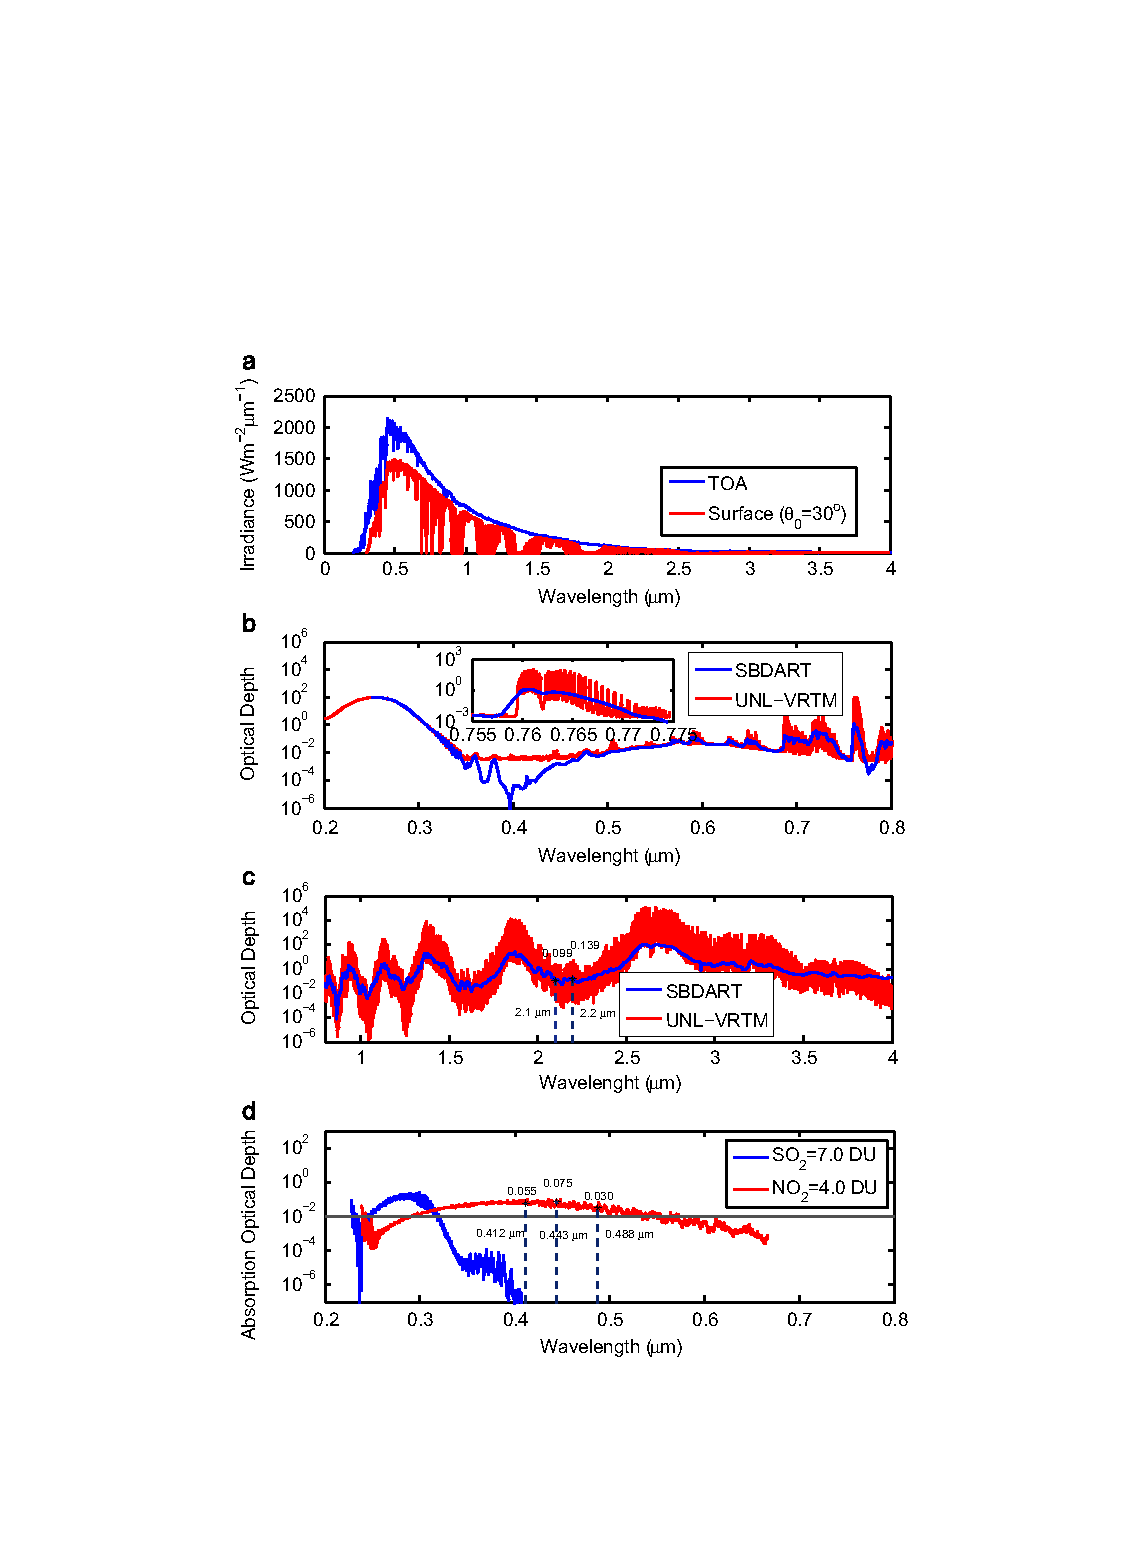
\includegraphics[width={0.8\textwidth}]{figures/unlvrtm1.pdf}
  \caption{(a) Downward solar spectral irradiance at the TOA and the
surface for solar zenith angle of 30$^\circ$. (b) Total-atmosphere gas
absorption optical depth in the range 0.2--0.8 $\mu$m. (c) Same as (b) but
for 0.8--4 $\mu$m. (d) Optical depth of \ce{SO2} and \ce{NO2} in
 polluted cases. Also shown in (b) and (c) are the optical depth computed 
from Santa Barbara DISORT Atmospheric Radiative Transfer (SBDART) model
\citep{Ricchiazzi98}. The mid-latitude summer atmospheric profile is 
assumed \citep{McClatchey72}. (Figure adopted from \citet{Wang14})}
  \label{fig:unlvrtm1}
\end{figure}

Figure \ref{fig:unlvrtm1}a shows the downward solar spectral irradiance 
at the top-of-atmosphere and at the surface for a solar zenith angle of
30$^\circ$. Spectral regions dominated by gas absorption can be 
clearly identified, including the \ce{O3} Hartley-Huggins bands 
in the UV, the \ce{O2}B band (0.69 $\mu$m) and \ce{O2}A band (0.76 
$\mu$m), as well as a number of water vapor bands. The
spectroscopic calculations shown in Figure \ref{fig:unlvrtm1} were 
performed at a resolution of 0.01 nm. In general this resolution is 
high enough to pick up fine structure in gas absorptions. 
In the UV below 300 nm, and in parts of the \ce{O2}A and \ce{O2}B 
bands, whole-atmosphere gas absorption optical depths can reach 
50 or more, and the downward irradiance is nearly zero
at the ground (Figure \ref{fig:unlvrtm1}b). The inset in Figure
\ref{fig:unlvrtm1}b shows a close-up view of the fine structure 
in absorption optical depth for the \ce{O2}A band, with
dual peaks centered at 0.761 $\mu$m and 0.764 $\mu$m, and a deep, 
narrow valley around 0.762 $\mu$m. Similarly, the continuum of water 
vapor absorption from the near-infrared to about 4 $\mu$m is also well 
simulated (Figure \ref{fig:unlvrtm1}c). Also of note is the 
non-negligible absorption of \ce{SO2} and \ce{NO2} in UV and blue
wavelength regions respectively (Figure \ref{fig:unlvrtm1}d). 
In urban regions, high \ce{SO2} and \ce{NO2} can together contribute 
optical depths of around 0.03--0.07 (Figure \ref{fig:unlvrtm1}d). 
Hence, in order to take advantage of low surface reflectance
in the UV and the use of deep-blue wavelengths for the retrieval of AOD
in urban regions, it is critical to treat absorption by \ce{SO2} and
\ce{NO2}. In contrast, calculations performed at moderate spectral 
resolution (such as those from Santa Barbara Discrete-Ordinate Atmospheric 
Radiative Transfer, or SBDART \citep{Ricchiazzi98}, shown as the blue 
lines in Figure \ref{fig:unlvrtm1}b and c) do not resolve fine-structure 
details, sometimes missing the absorption lines for \ce{SO2} or \ce{NO2}, 
and in general producing significant underestimation of optical depths 
in the \ce{O2}A band.

\begin{figure}[t]
  \centering
  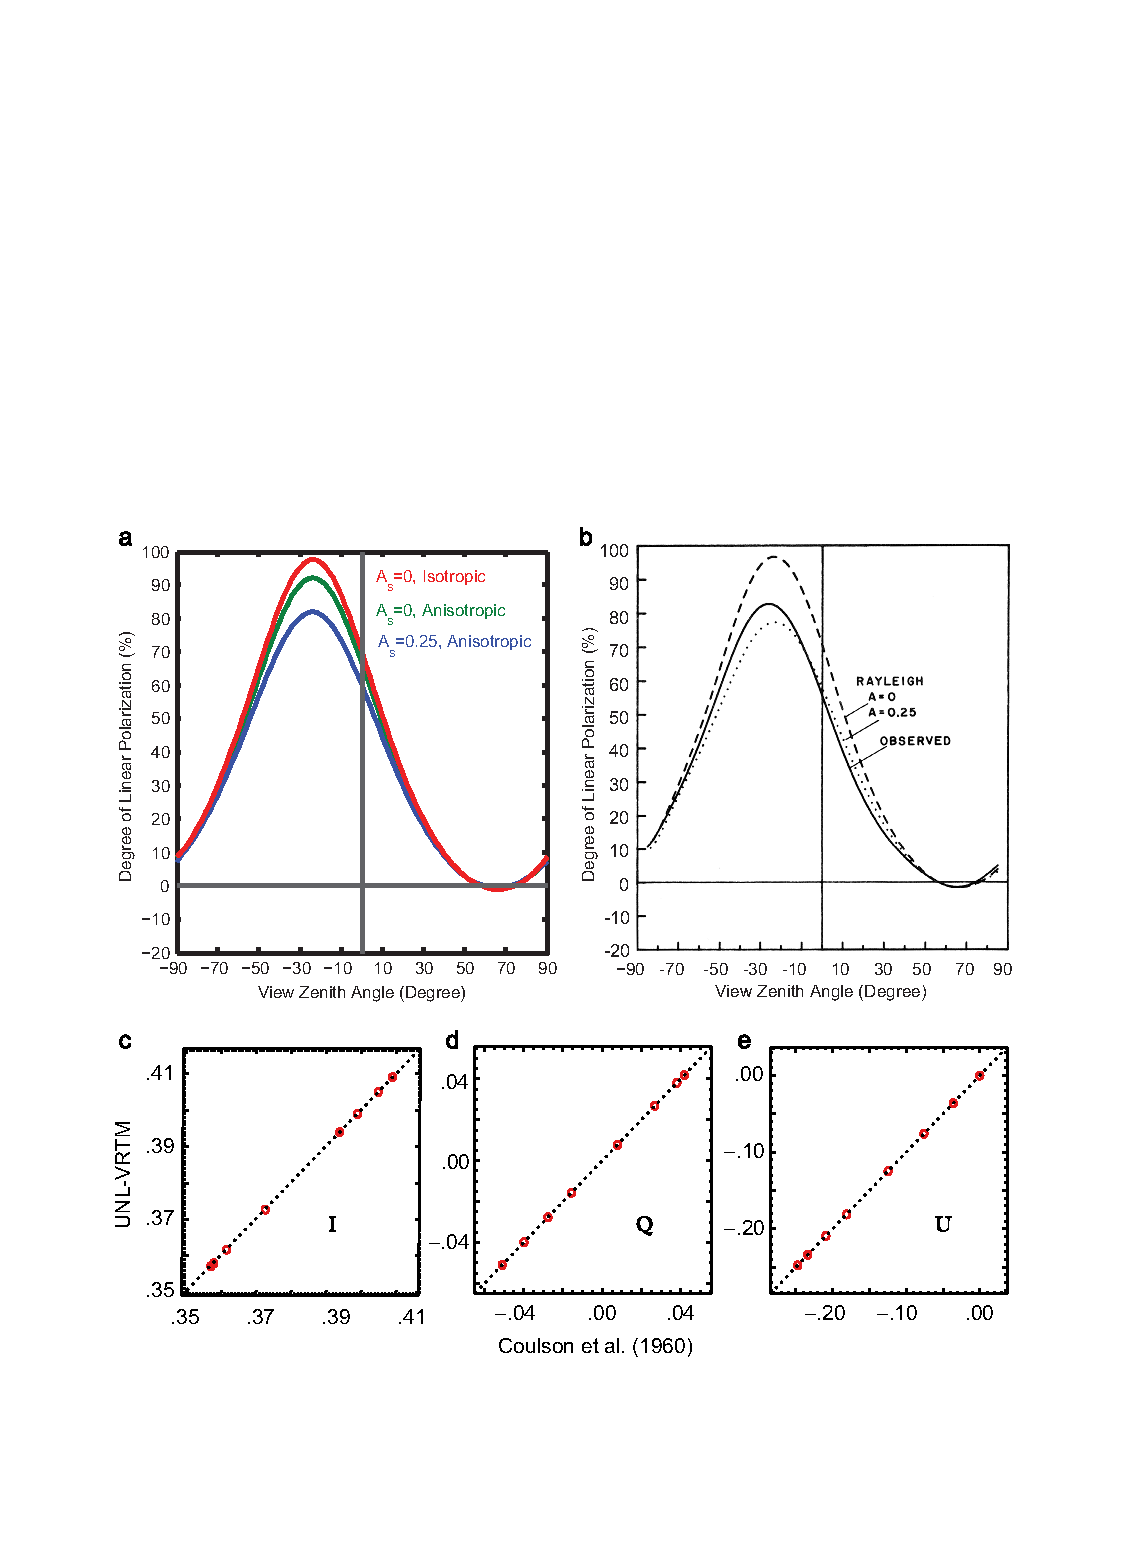
\includegraphics[width={0.8\textwidth}]{figures/unlvrtm2.pdf}
  \caption{Degree of linear polarization ($-Q/I$) of downward radiation
for a pure Rayleigh atmosphere: (a) computed by UNL-VRTM for the case
analyzed in Figure 5.7 of \citet{Coulson88} and shown here as (b). (c)--(e)
shows the comparisons of $I$, $Q$, and $U$ computed by \citet{Coulson60} and
those from UNL-VRTM. In (a) and (b), As represents the surface albedo
value. In (c) and (d), the calculation is for $\tau=1.0$, surface albedo
is 0.25, $\cos{\theta_0}=0.8$, and for 8 different viewing angles.
(Figure adopted from \citet{Wang14}) }
  \label{fig:unlvrtm2}
\end{figure}

\begin{figure}[t]
  \centering
  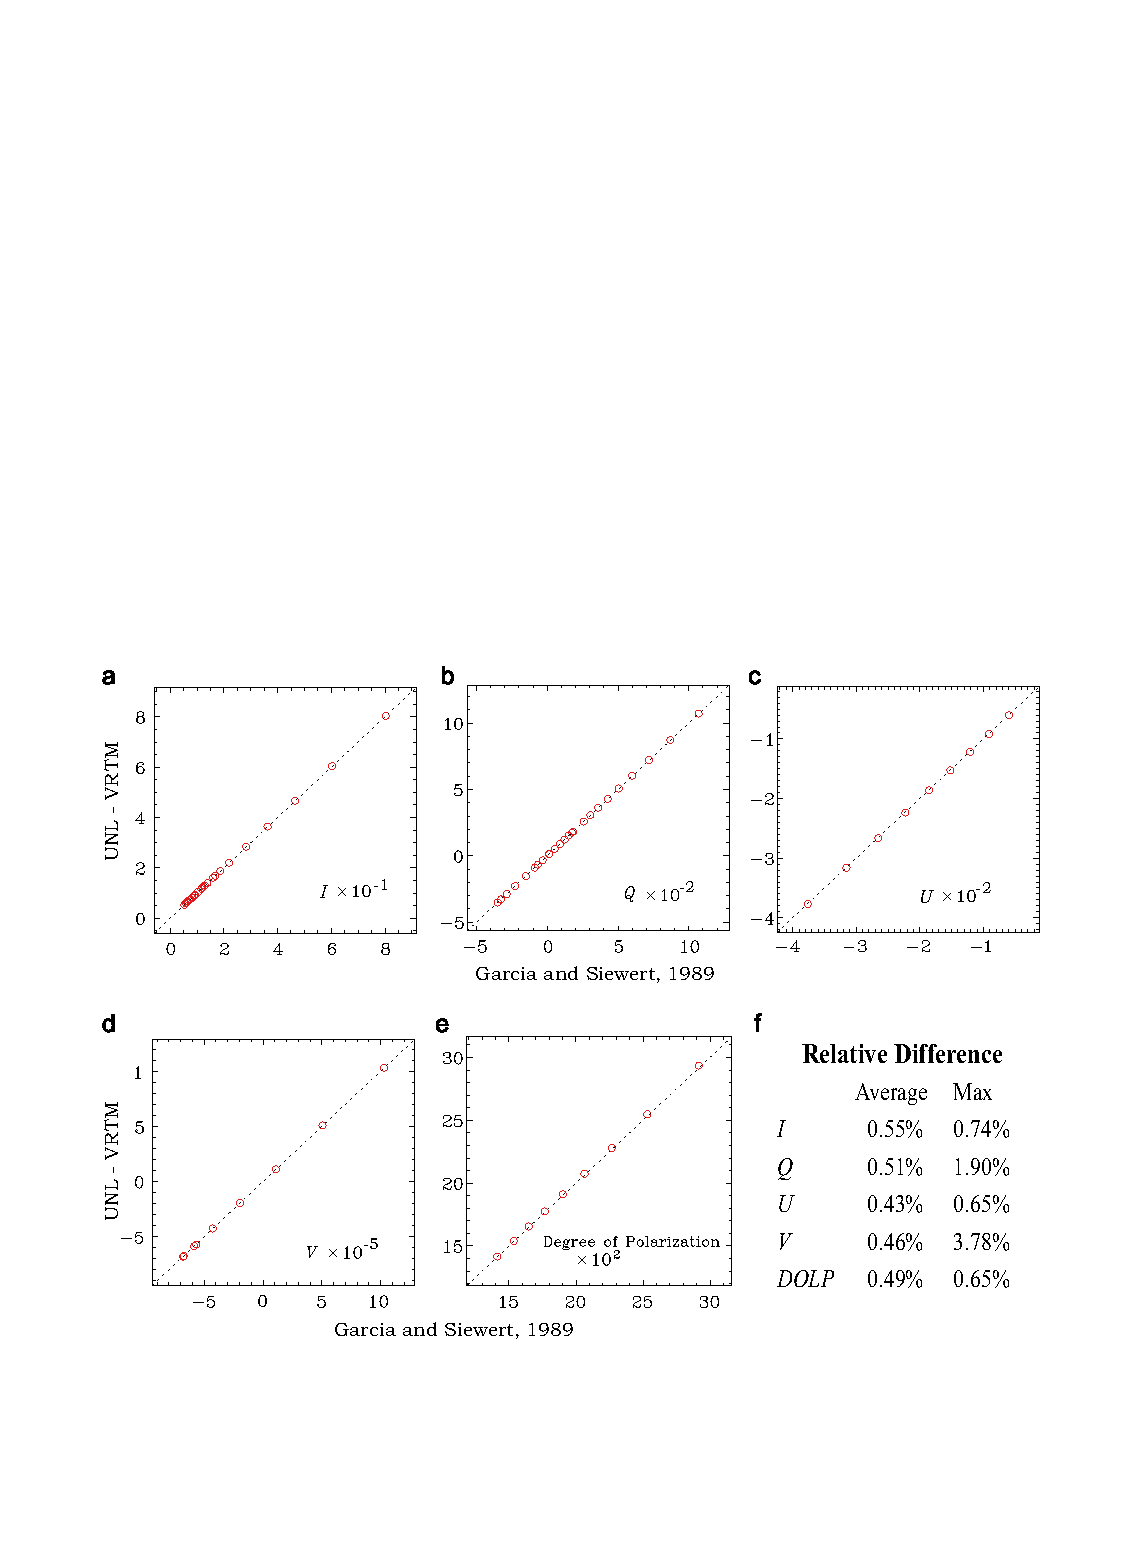
\includegraphics[width={0.8\textwidth}]{figures/unlvrtm3.pdf}
  \caption{Counterparts in Tables 3--10 of \citet{Garcia89} for
upwelling radiation on the top of the same atmospheric conditions of
aerosol scattering. No gas absorption and Rayleigh scattering are
considered. Note that compared here are $I$ and $Q$ values reported 
in \citet{Garcia89} for 9 view angles (with cosine values from 0.1 
to 0.9 at equal spacing of 0.1) and 3 relative azimuth angles 
(0, $\pi/2$, and $\pi$), which yields a total of 27 data points. 
For $U$ and $V$, their values are reported for the same 9 viewing angles 
but for one relative azimuth angle ($\pi/2$) only. 
The calculation is performed at wavelength of 951 nm and $\tau$ of 1.0, 
and aerosol size distribution parameters $\reff=0.2$, 
$\veff=0.07$, refractive index $\mreal=1.44$, and SSA of 0.99.
(Figure adopted from \citet{Wang14}) }
  \label{fig:unlvrtm3}
\end{figure}

Figure \ref{fig:unlvrtm2} shows the calculation of the degree of linear 
polarization (DOLP) of downward radiation in a pure Rayleigh scattering 
atmosphere. The solid blue line in Figure \ref{fig:unlvrtm2}a (dotted 
line in Figure \ref{fig:unlvrtm2}b) reproduces the theoretical results 
shown in Figure 5.7 of \citet{Coulson88}, which was used to interpret 
the DOLP measured at Mauna Loa Observatory on February 19, 1977. 
Furthermore, Figure \ref{fig:unlvrtm2}a shows that the anisotropy in
Rayleigh scattering reduces the peak DOLP by 5\% (e.g., the difference
between the green and red lines) at 0.7 $\mu$m. Surface reflection and its
concomitant increase of atmosphere scattering will decrease the DOLP of
downward radiation. An increase of surface reflectance from 0 to 0.25
decreases the peak DOLP by 10\%.

Quantitatively, the Stokes-vector $I$, $Q$, and $U$ components computed with
UNL-VRTM differ from their counterparts found in the tables by
\citet{Coulson60} by average (relative) deviations of $1.9\times 10^{-4}$
(0.05\%), $2\times 10^{-5}$ (0.14\%), and $4\times 10^{-5}$ (0.03\%), 
respectively (Figure \ref{fig:unlvrtm2}c--e). These
differences are similar to the values $2.1\times 10^{-4}$, $9\times
10^{-5}$, and $4\times 7^{-5}$ identified by \citet{Evans91}. More recently,
Rayleigh-atmosphere benchmark results have been re-computed by
\citet{Vijay12} to a much higher degree of accuracy; this work also
included benchmarking of the VLIDORT model.

Figure \ref{fig:unlvrtm3} shows benchmark calculations of four 
Stokes parameters for radiative transfer in an aerosol-only atmosphere.
\citet{Garcia89} documented their results for unpolarized incident 
radiation at 951 nm and $cos{\Theta_0}$ of 0.2, for an atmosphere with a
Lambertian reflectance of 0.1. The aerosols in that atmosphere were
assumed to satisfy a gamma-function size distribution with $\reff$ of
0.2 $\mu$m and $\veff$ of 0.07, and a refractive index yielding an 
aerosol single scattering albedo of 0.99. Compared to their results, 
the Stokes parameters computed by UNL-VRTM show relative differences 
of less than 0.6\%, with maximum relative differences 
(at certain viewing geometries) of up to 2\% for $Q$ and 3.8\% for $V$. 
The DOLP computed from the UNL-VRTM (with 15 streams for the hemisphere) 
and documented by \citet{Garcia89} (with 3 streams) differ on average 
by 0.5\%, with a maximum relative difference of 0.65\%.

The simultaneous calculation of analytic Jacobians of the four Stokes
parameters with respect to the aerosol optical depth, size parameters,
refractive indices, and aerosol-loading peak height for both fine and
coarse model aerosols may be validated against Jacobians calculated
using the finite difference method (Figures \ref{fig:unlvrtm4} and
\ref{fig:unlvrtm5}). Overall, results from the two methods are 
highly correlated as seen in the scatter plots
shown in these figures. Relative differences in all comparisons are
less than 0.5\%, and in many cases the differences are less than 0.05\%.

\begin{landscape}
\begin{figure}[p]
  \centering
  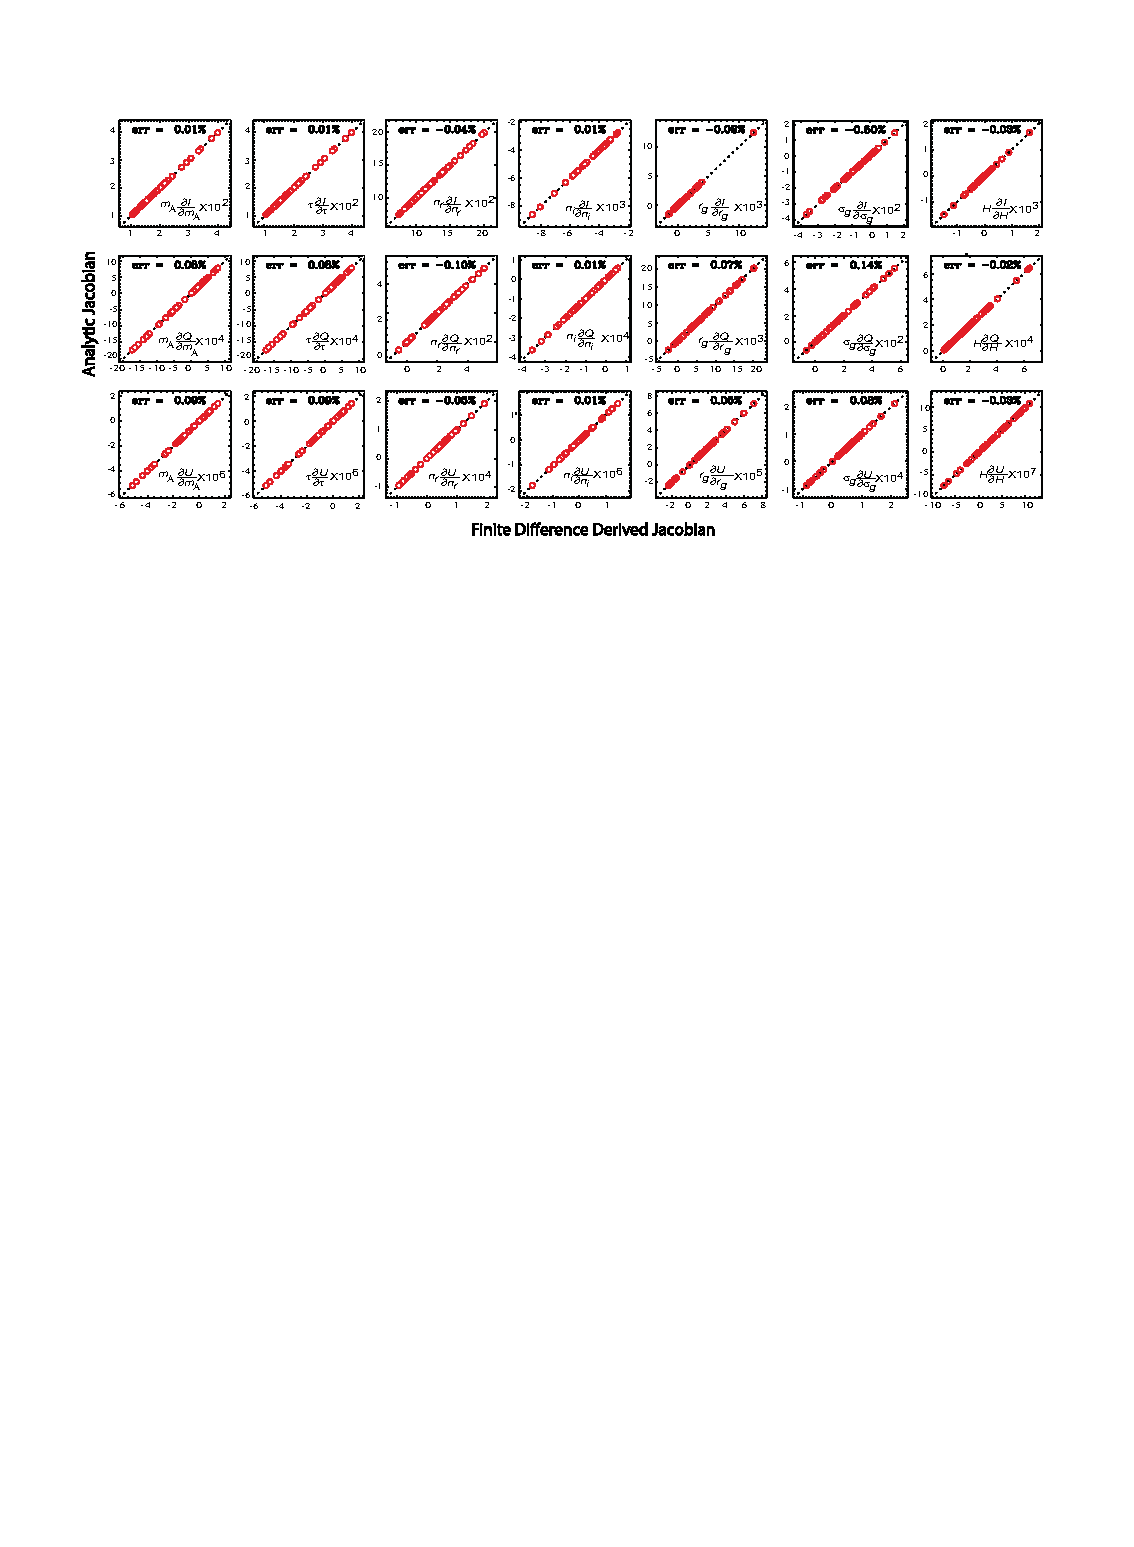
\includegraphics[width={1.4\textwidth}]{figures/unlvrtm4.pdf}
  \caption{Intercomparison of Jacobians ($\ptxi/\partial\ln{x}$) 
calculated with UNL-VRTM using the analytical method (y-axis) with 
those computed from UNL-VRTM using finite-difference estimates (x-axis). 
Here $\xi$ is one of the Stokes parameters: $I$ (top row), $Q$
(middle row), and $U$ (last row). x is one of 7 parameters associated 
with fine-mode aerosols: mass concentration $m_\text{A}$, $\taua$,
$\mreal$, $\mimag$, $\rg$ and $\sg$ (of the lognormal PSD), and height
($H$) of peak aerosol concentration in the vertical. Note,
the calculation is done for an atmosphere containing both fine- 
and coarse-mode aerosols as described in \citet{Hess98}.
(Figure adopted from \citet{Wang14}) }
  \label{fig:unlvrtm4}
\end{figure}
\end{landscape}

\begin{landscape}
\begin{figure}[p]
  \centering
  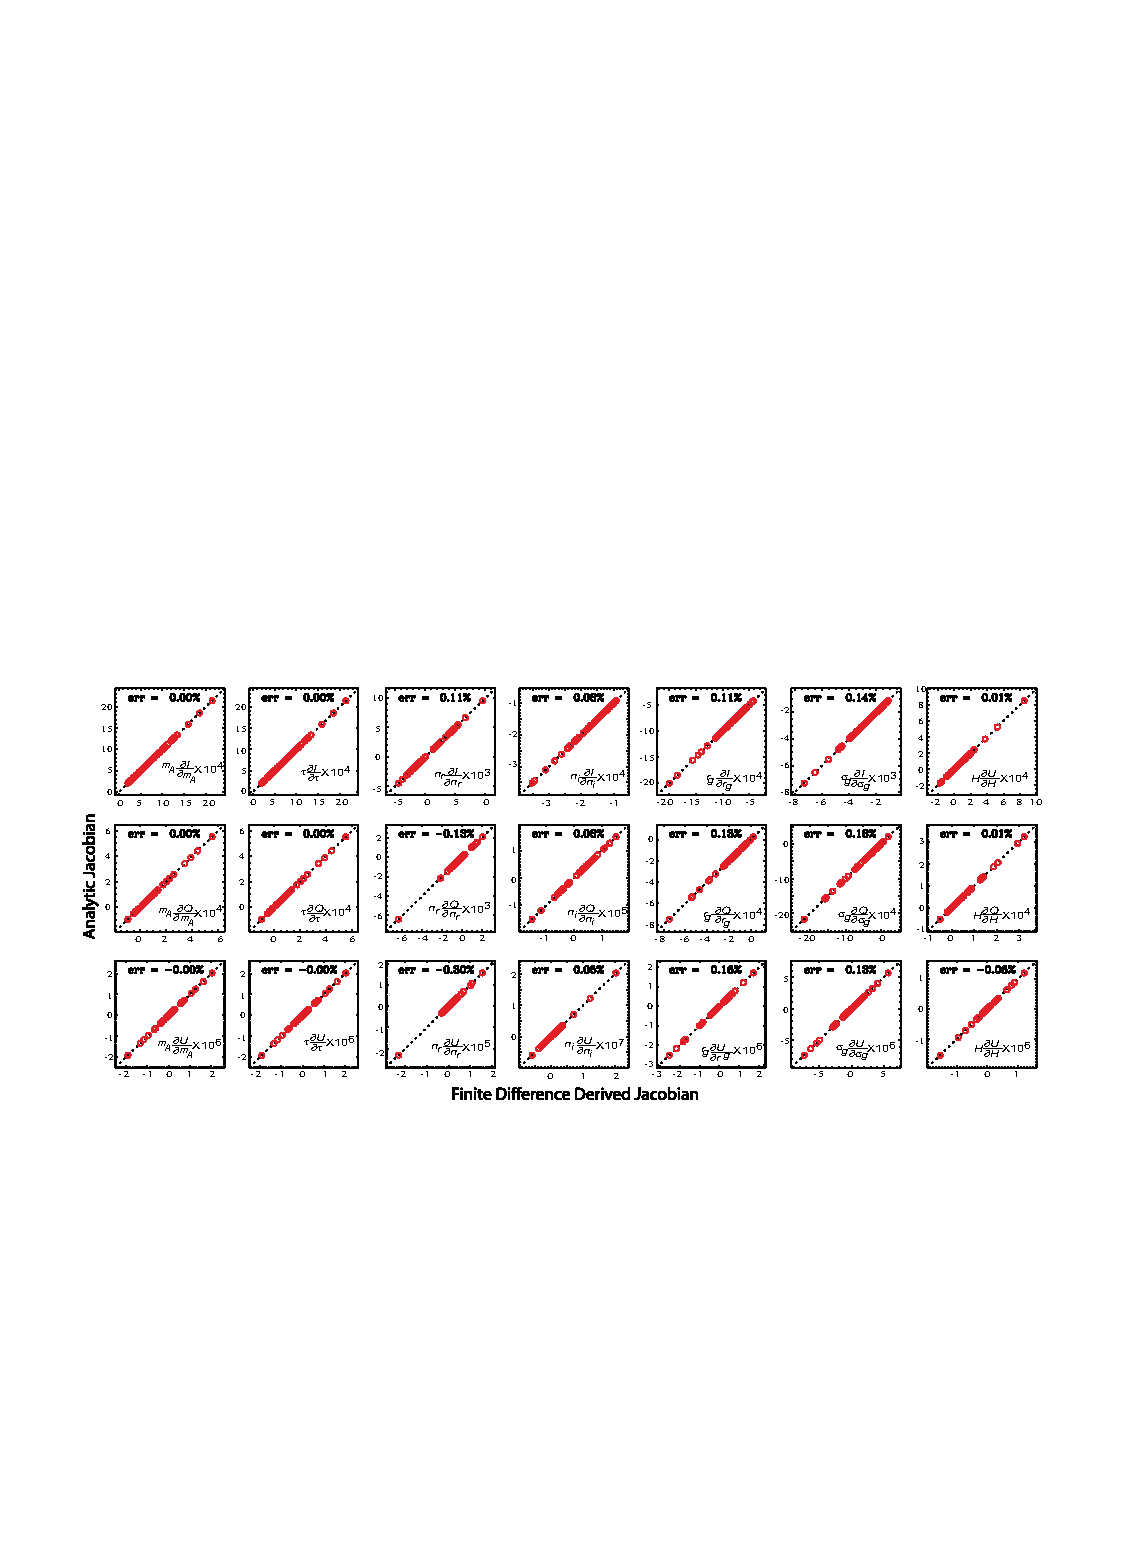
\includegraphics[width={1.4\textwidth}]{figures/unlvrtm5.pdf}
  \caption{Same as in Fig. 5, but for coarse mode aerosols.
(Figure adopted from \citet{Wang14}) }
  \label{fig:unlvrtm5}
\end{figure}
\end{landscape}
 
%%
\chapter{Inversion Algorithm} \label{ch:algorithm}

\section{General sturcture}

Basic formulation of inverse problem; sturcture of the algorithm.

\section{Combine a priori and smoothness constraints}

\section{Statistical optimized inversion}

\section{Retrieval Error Characertization}

\section{Qaulity Control of Measurements}


 
%% 
\chapter{Information Content Analysis}

\section{Introduction}

The AERONET collects not only the multi-spectral and multi-angular radiance
observations, but also the state of light polarization from various viewing
angles over many sites (section \ref{subsec:cimel318}). 
Unfortunately, the potential of AERONET polarization
measurements in retrieving aerosol microphysical parameters has not been fully
exploited. Polarization measurements contain valuable information about aerosol
microphysical properties \citep{Mishchenko97,Cairns97}, as
the polarization of light is highly sensitive to the aerosol size and
refractive index \citep{Hansen74}. Several studies have emphasized the
usefulness of the polarimetric observations taken by the ground-based
instruments \citep{Cairns97, Boesche06, Emde10, Zeng08}.  
\citet{Vermeulen00} presented a two-step method to retrieve
aerosol microphysical properties from polarized radiances: first, the single
scattering albedo and the natural and polarized phase functions were retrieved
from transmission and almucantar radiances and polarization in the principal
plane; second, the aerosol PSD and refractive index were then derived. With the
current AERONET inversion algorithm, \citet{Dubovik06} conducted a case
study using polarization data in a UAE$^2$ (Unified Aerosol Experiment-United 
Arab Emirates) field campaign \citep{Reid08}. \citet{Li09} extended the
inversion algorithm of \citet{Dubovik06} to include multi-spectral
polarization and demonstrated improved retrievals in real part aerosol
refractive index for fine particles and the fraction of spherical particles.

However, questions regarding the use of AERONET polarimetric observations for
retrieving aerosol microphysical parameters remain unresolved: (1) Practically,
do the existing AERONET photo-polarimetric measurements have any potential to
improve the retrieval of aerosol information content that we now routinely
obtain from radiance measurement only? and (2) Hypothetically, how can future
upgrades of AERONET photo-polarimetric measurements and inversion algorithm
maximize the retrieval information content of aerosols? Answering these two
questions is not only relevant to the future AERONET instrumentation design,
but also for the ground-based passive polarimetric remote sensing of aerosols
in general. 

%% Table of a priori
\begin{table}[b]
  \centering
  \small
  \caption{The aerosol parameters defined for both fine and coarse aerosol
modes\textsuperscript{a}.}
  \label{tab:infox}
  \begin{tabular}{p{2em} C{3em}  C{3em} C{9em} C{9em} C{7em} }
  \toprule
  Mode  & $\reff$($\mu$m) & $\veff$ & $\mathbf{m}_\text{r}$ &
$\mathbf{m}_\text{i}$ & $\assa$ \\
  \midrule
  Fine & 0.21 \newline (80\%) & .25 \newline (80\%) &
    1.44, 1.44, 1.43, 1.42 \newline (.15) &
    .009, .011, .012, .011 \newline (.01) &
    .95, .93, .92, .91 \\
  Coarse & 1.90 \newline (80\%) & .41 \newline (80\%) &
    1.56, 1.55, 1.54, 1.54 \newline (.15) &
    .004, .003, .003, .002 \newline (.005) &
    .84, .91, .93, .96 \\
  \bottomrule
  \multicolumn{6}{m{35em}}{\textsuperscript{a}The complex refractive index
$\mathbf{m}_\text{r}-\mathbf{m}_\text{i}i$, and single scattering albedo
$\assa$ are reported at 440, 675, 870, and 1020 nm. Bracketed values are
assumed a priori error in relative for $\reff$ and $\veff$ and in absolute
for $\mathbf{m}_\text{r}$, $\mathbf{m}_\text{i}$, and $\assa$. }
  \end{tabular}
\end{table}

In this chapter, we seek to answer above questions from a theoretical 
perspective (section \ref{subsec:infotheory}) by investigating the available 
information contained in the AERONET measurements with and without the 
inclusion of polarization data. This investigation is to
provide the a theoretical foundation to support actual
algorithm development for using polarimetric data for aerosol retrievals. 
The structure of this chapter is as follows. In section \ref{sec:expdesign}, 
we describe the experimental design on the aerosol models, error 
characteristics of \textit{a priori} and AERONET measurements. Section
\ref{sec:inforesult} presents the results of information content and error
analysis. In section \ref{sec:infosensi}, we investigate the sensitivity of
retrieval uncertainties in aerosol parameters with respect to the aerosol
loading and fine/coarse aerosol characteristics. Finally, we summarize in
section \ref{sec:infosummary} the general findings of this study and 
implications for practical algorithm development. 

\section{Experimental Design} \label{sec:expdesign}

\subsection{\textit{a priori} characteritics}

The state vector $\xbf$ comprises 22 (11 pairs) retrieved parameters,
namely, the columnar volume concentration $V_0$, the effective radius $\reff$, the
effective variance $\veff$, and the complex refractive index $\mreal+\mimag{i}$ 
at 440, 675, 870, and 1020 nm (section \ref{subsec:xy}). These 11 pairs of 
parameters charcterizing aerosol properties in the both fine and coarse 
aerosol modes; each mode follows a lognormal PSD function. Table \ref{tab:infox} 
displays aerosol size parameters, refractive indices, and single scattering 
albedo for each size mode adopted for error and information analysis; 
also showed in brackets are their associated \textit{a priori} uncertainties. 
The fine-mode particles are corresponding to water-soluble aerosols 
obtained from OPAC database \citep{Hess98} with updates by \citet{Drury10}, 
while the coarse-mode is preassembly for large spherical particles with 
refractive index from \citet{Patterson77,Wagner12}.

%% Table of aerosol optical properties
\begin{table}[b]
  \centering
  \small
  \caption{The aerosol scenarios adapted for numerical
experiments\textsuperscript{a}.}
  \label{tab:infoopt}
  \begin{tabular}{p{8em} C{1em} C{1em} C{7em} C{7em} C{1em} C{7em} }
  \toprule
  Aerosol type & $V_0$ & $\fmfv$ & $\taua$ &
$\fmftau$ & AE & $\assa$ \\
  \midrule
  Fine-dominated & .15 & .8 & 1.0, .58, .36, .25 &
    .97, .95, .92, .88 & 1.5 & .95, .93, .92, .91 \\
  Well-mixed & .22 & .5 & 1.0, .61, .41, .32 &
    .90, .83, .74, .65 & 1.3 & .94, .93, .92, .93 \\
  Coarse-dominated &.43 &.2 & 1.0, .71, .57, .50 &
    .69, .55, .42, .32 & .82 & .91, .92, .92, .94 \\
  \bottomrule
  \multicolumn{7}{m{35em}}{\textsuperscript{a}Values for $\taua$, $\assa$, and
$\fmftau$ are listed respectively for spectral wavelength of
440, 675, 870, and 1020 nm. The AE is reported between 440 and 870 nm. $V_0$ is 
in the unit of $\mu$m$^3\mu$m$^{-2}$}
  \end{tabular}
\end{table}

In order to include various atmospheric conditions, we simulate three types of
aerosols---each with different relative percentage between the coarse and fine
modes---(I) fine particles dominated, (II) well mixed, and (III) coarse
particles dominated. As listed in Table \ref{tab:infoopt} and illustrated 
in Figure \ref{fig:infopsd}, fine-mode
fractions in terms of volume ($\fmfv$) are defined as 0.8, 0.5, and 0.2 for these
three types, respectively. Aerosol volumes are scaled as necessary to maintain
a normalized AOD at 440 nm corresponding to a moderate hazy condition
($\tau_{440}=1.0$). The spectral aerosol optical depths $\taua$, 
single scattering albedo $\assa$, and the Ångström exponent (AE) 
are calculated and also shown in Table \ref{tab:infoopt}. 

\begin{figure}[t]
  \centering
  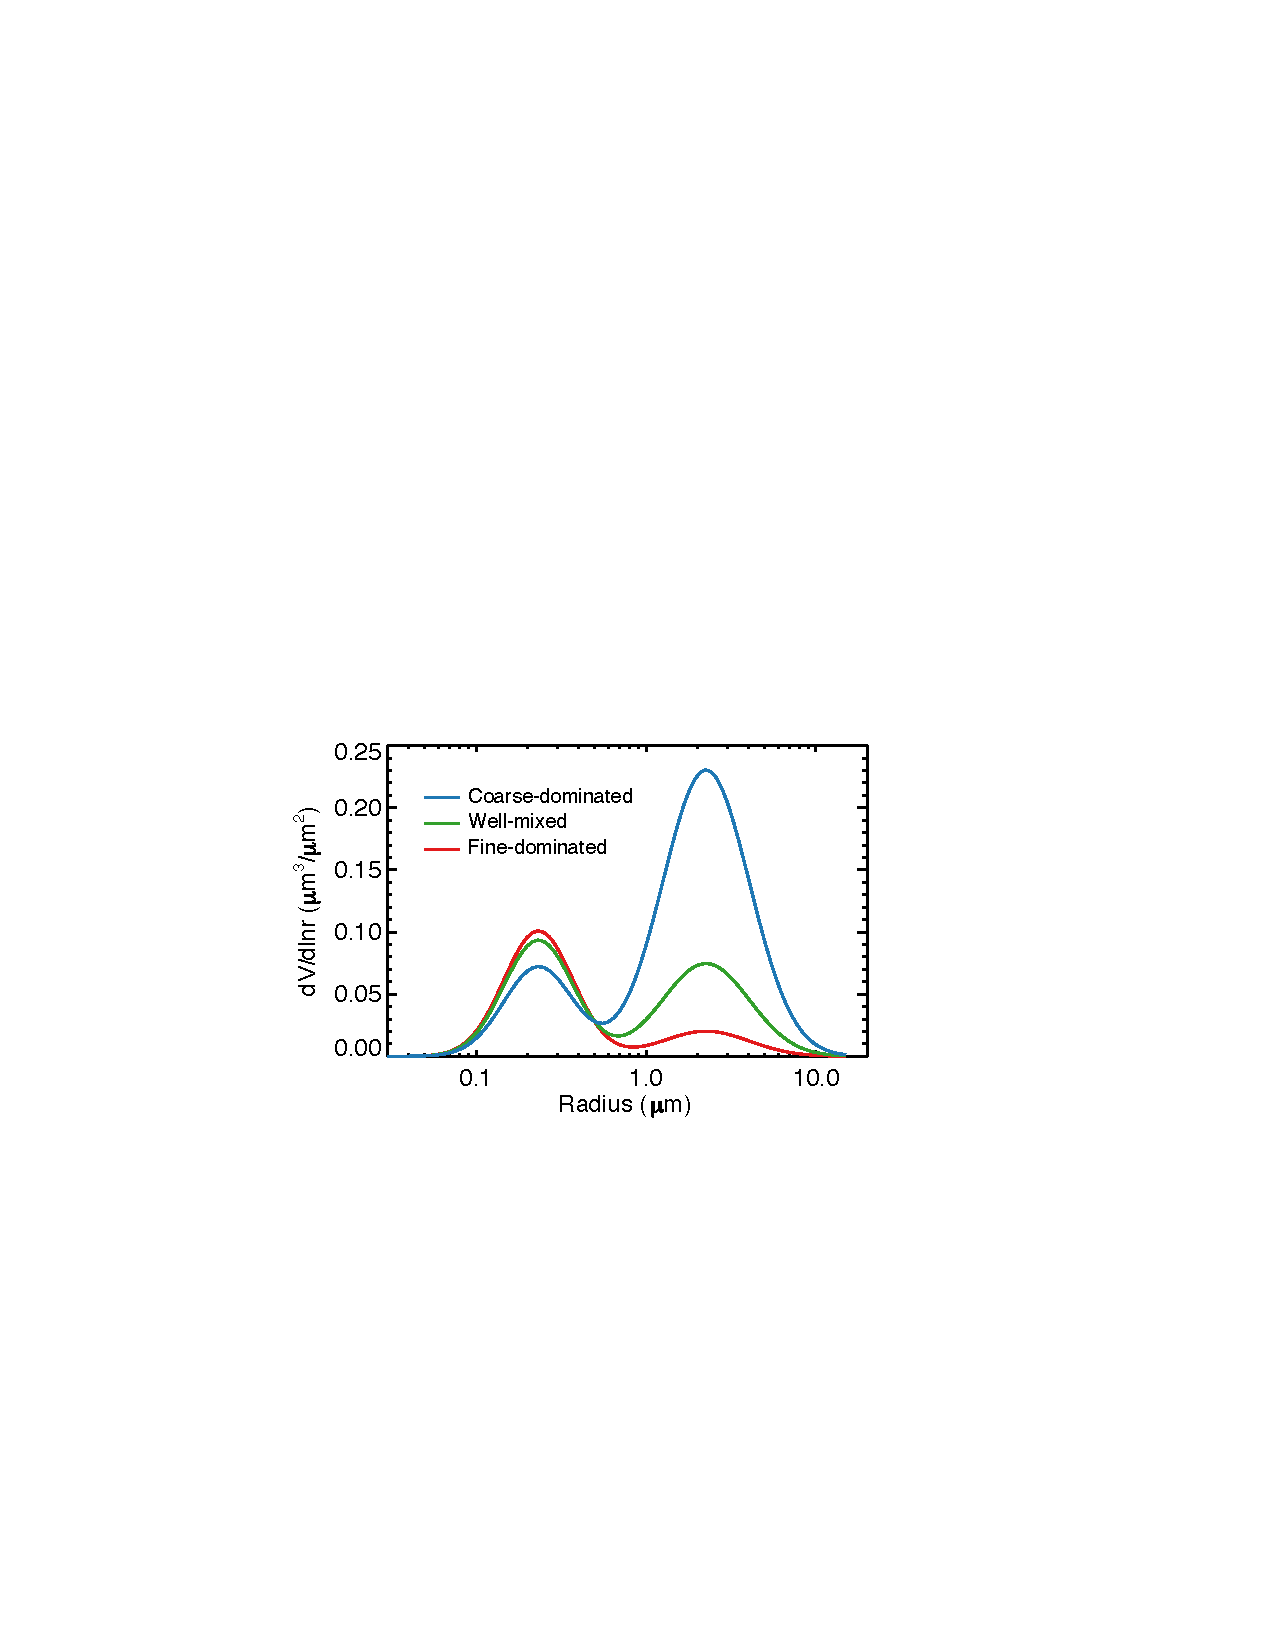
\includegraphics[width={0.75\textwidth}]{figures/info01.pdf}
  \caption{Volume size distribution for the aerosol types adopted for the
information analysis. Relevant aerosol parameters are summarized in the Tables
\ref{tab:infox} and \ref{tab:infoopt}.}
  \label{fig:infopsd}
\end{figure}

\subsection{Synthetic observations}

As described in section \ref{subsec:cimel318} and Table \ref{tab:cimel318}, 
The SunPhotometer equipped at AERONET sites routinely measures direct and
diffuse (sky) solar radiances and optionally the mono-band light 
polarization \citep{Holben98}. Recently, multi-spectral polarizations 
have also been taken with a newer-generation SunPhotometer (CIMEL CE318-DP) 
at some sites \citep{Li09} and the UAE$^2$ fields campaign \citet{Reid08}.
 Here we focus our study on using multi-spectral polarizations 
for the inversion of aerosol parameters. 

In order to investigate the merit of synergizing various observations in the
inversion, we define four different scenarios of observation vectors, i.e., I1,
I2, P1, and P2 as summarized in the Table 1. The observation vector in scenario
I1 comprises direct sun AODs and solar almucantar radiances ($\ialm$) at 440,
675, 870, and 1020 nm. Scenario I2 includes measurements in scenario A and the
total radiances ($\ipp$) at the same four wavelengths observed in the solar
principal-plane. Observations in scenario P1 are defined to further include
$\dolppp$ at those four wavelengths. Lastly, scenario P2 observations comprise
basic measurements in scenario I1 plus almucantar polarization ($\dolpalm$) at
same wavelengths. The $\dolpalm$ is not routinely measured by any current
SunPhotometer, but we include it for a comparative analysis. Measurements
defined in scenario I1 represent observations used by the current AERONET
operational inversion and thus serves as a control experiment. From scenario
I2, we can investigate the synergy of radiances in both the solar almucantar
and solar principal-plane. Scans in the solar principal-plane can achieve
larger scattering angles and thus may contain additional scattering
information. And with scenarios P1 and P2 we will be able to evaluate the
potential of adding polarization in the inversion. 

%% Table of aerosol optical properties
\begin{table}[t]
  \centering
  \small
  \caption{List of scenarios of AERONET observations used for
information content analysis.}
  \label{tab:infoy}
  \begin{tabular}{p{4em} p{11em} p{21em} }
  \toprule
  Scenario & Observations included\textsuperscript{a} & Remark  \\
  \midrule
  I1 & $\taua$, and $\ialm$ & Observations used in \Dub algorithm \\
  I2 & $\taua$, $\ialm$, and $\ipp$ & Scenario I1 plus principal-plane
radiances \\
  P1 & $\taua$, $\ialm$, $\ipp$ and $\dolppp$ & Scenario I2 plus
principal-plane polarization\\
  P2 & $\taua$, $\ialm$, and $\dolpalm$ & Scenario I1 plus almucantar
polarization \\
  \bottomrule
  \multicolumn{3}{m{35em}}{\textsuperscript{a}Variables are for four spectral
wavelengths, i.e., 440, 675, 870, and 1020 nm.}
  \end{tabular}
\end{table}

We exclude $\ippl$ (Table \ref{tab:cimel318}) in our analysis because 
sky radiance in the solar principal plane can be also obtained during the 
polarization scan ($\ipp$). $\ippl$ and $\ipp$
are different in the viewing-angle sequences, but they generally share a
similar range of scattering angles. Thus, one is redundant for the other. We
also exclude analysis for monochromatic polarization (at 870 nm) current
measured on many AERONET sites, because single-band polarization measurements
contain much less information than multi-band ones and newer generation
SunPhotometers with multi-band polarization capacity will be deployed at more
AERONET sites. 

\section{Results} \label{sec:inforesult}

Following the approach stated in section \ref{sec:invtheory}, 
we have simulated the AERONET photo-polarimetric measurements under various 
solar zenith angles from 40$^\circ$ to 75$^\circ$ for the three 
defined aerosol types (Table \ref{tab:infoopt}). The simulated radiances 
($\ialm$) on the solar almucantar plane and the degree of linear 
polarization ($\dolppp$) on the solar principal plane are illustrated in 
Figure \ref{fig:infosimu} for aerosols of type II with solar zenith angle of 
55$^\circ$. These simulations for other aerosol types and other
solar zenith angles are of similar pattern. According to Figure
\ref{fig:infosimu}a, $\ialm$ decreases as the scattering angle increases, 
resulting from forward-dominated scattering phase function of aerosol 
particles. The maximum $\dolppp$ takes place at the scattering angle of 
90$^\circ$ as a result of composite effect of Rayleigh and aerosol scattering, 
while the smaller $\dolppp$ values dominates at the small scattering angles 
because of the predominance of diffracted light (Figure \ref{fig:infosimu}b).
With the synthetic data and relevant error characterizations, we have computed
the EN Jacobian matrix, DFS, and a posteriori error to evaluate the capacity of
AERONET measurements in inferring aerosol microphysical properties. Our
analysis mainly focuses on the comparison of those quantities between
measurements with and without including polarization, so that we can understand
the importance of adding polarization for the retrieval.  

\begin{figure}[t]
  \centering
  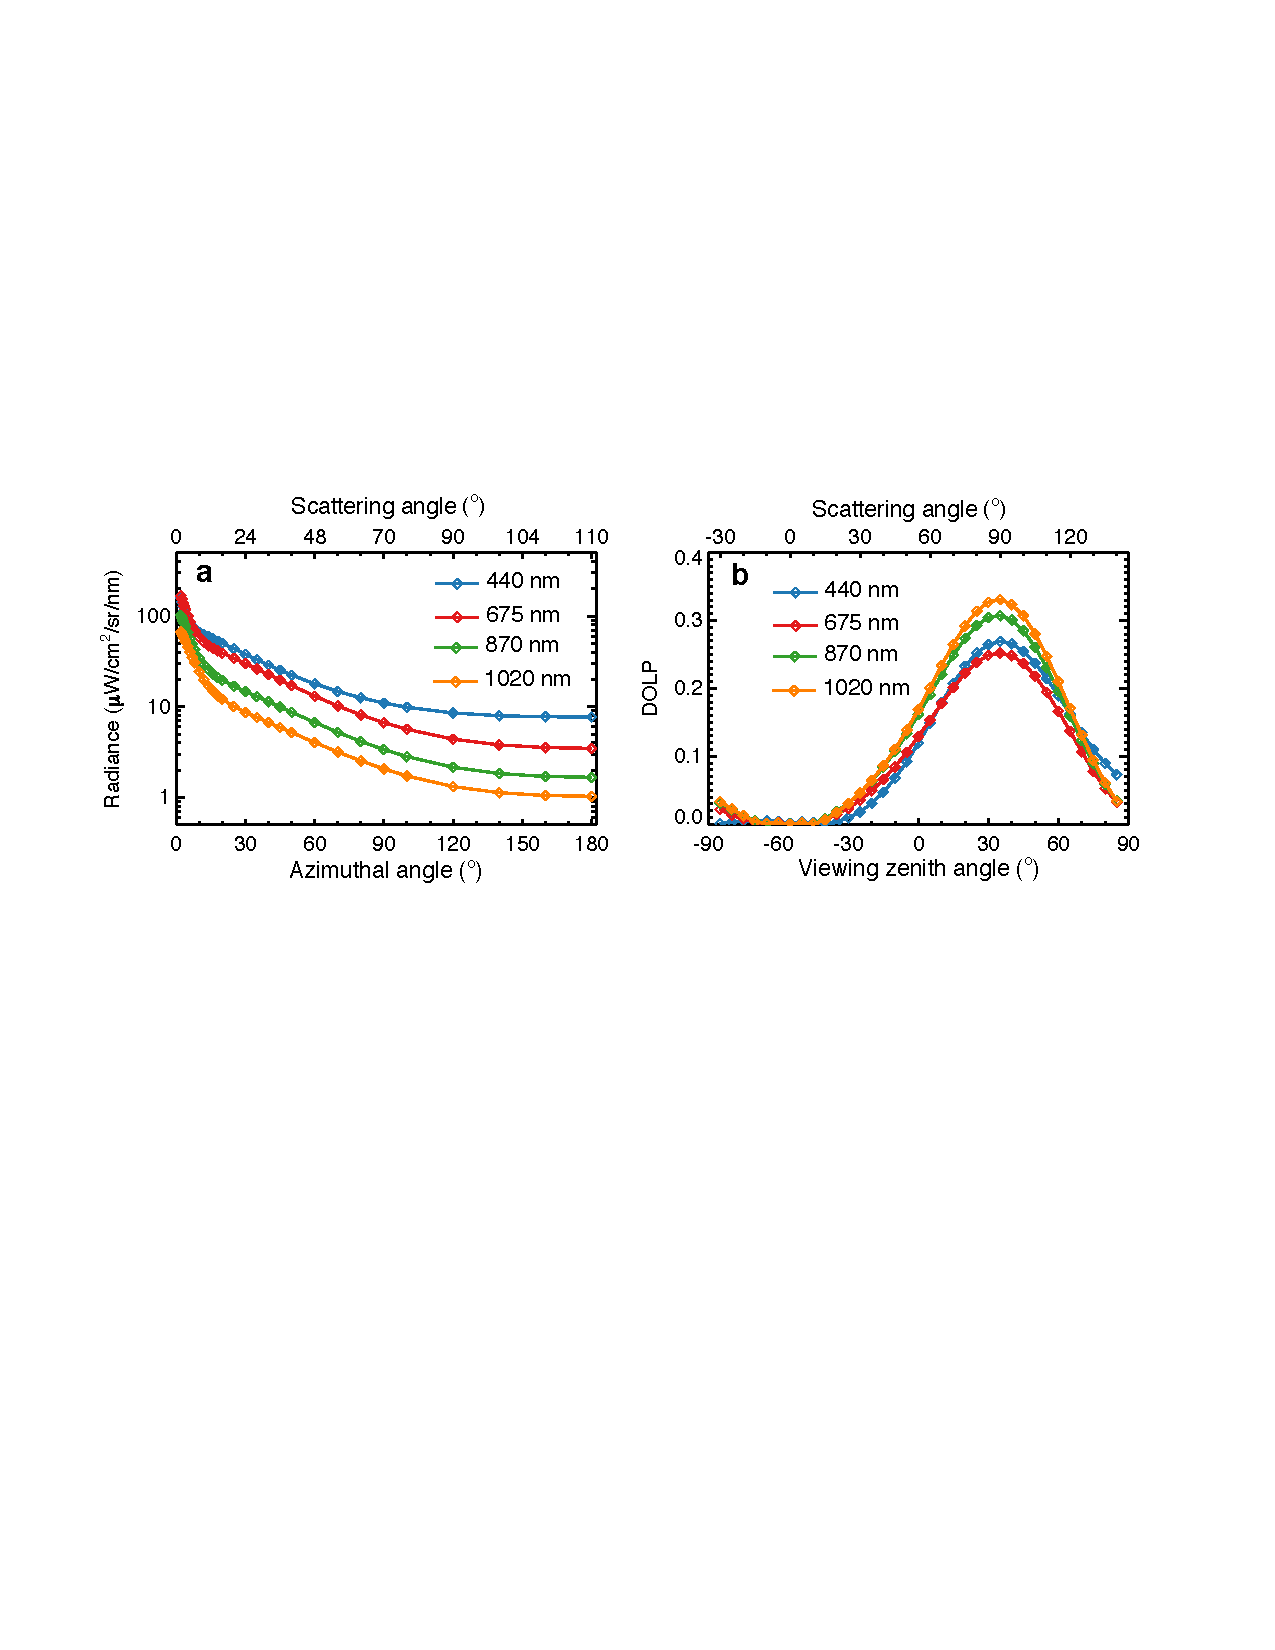
\includegraphics[width={\textwidth}]{figures/info02.pdf}
  \caption{(a) Simulated radiances in the solar almucantar plane as a function
of azimuth angle. (b) Simulated degree of linear polarization (DOLP) in the
solar principal plane as a function of view zenith angle. Simulations are for
the well-mixed aerosol type with columnar AOD of 1.0 at 440 nm as shown in the
Table \ref{tab:infoopt}. Solar zenith angle is 55$^\circ$ and top abscissas 
show corresponding scattering angles.}
  \label{fig:infosimu}
\end{figure}

\subsection{Error-normalized (EN) Jacobian matrix} \label{subsec:enj}

We compare the EN Jacobians for the $\ialm$ and $\dolppp$ in both 
Figure \ref{fig:infoenjf} and Figure \ref{fig:infoenjc} to disclose the 
importance of $\dolppp$ measurements to the retrieval. Distinct patterns of EN 
Jacobians can be found between the $\dolppp$ and $\ialm$ over the
scattering angle. As shown in Figures \ref{fig:infoenjf}a and
\ref{fig:infoenjc}a, the radiance at scattering angles less than
$\sim$10$^\circ$ decreases with increasing fine-mode aerosol loading (e.g.
negative $\partial\ialm/\partial{V_0}$) and increases with increasing 
coarse-mode aerosol loading (e.g. positive $\partial\ialm/\partial{V_0}$), 
whereas the sensitivity of the $\ialm$ to $V_0$ at larger scattering angles is 
larger positive in the fine mode and less positive in the coarse mode. 
It is because large particles scatter more radiation than small particles at 
near-forward scattering angles \citep{vandeHulst81}. In contrast, the $\dolppp$ 
presents profound sensitivity to the $V_0$ of aerosol in both modes at the 
scattering angles between 45$^\circ$ and 135$^\circ$ (Figures 
\ref{fig:infoenjf}f and \ref{fig:infoenjc}f). 

%% Figure EN Jacobian fine mode
\begin{figure}[p]
  \centering
  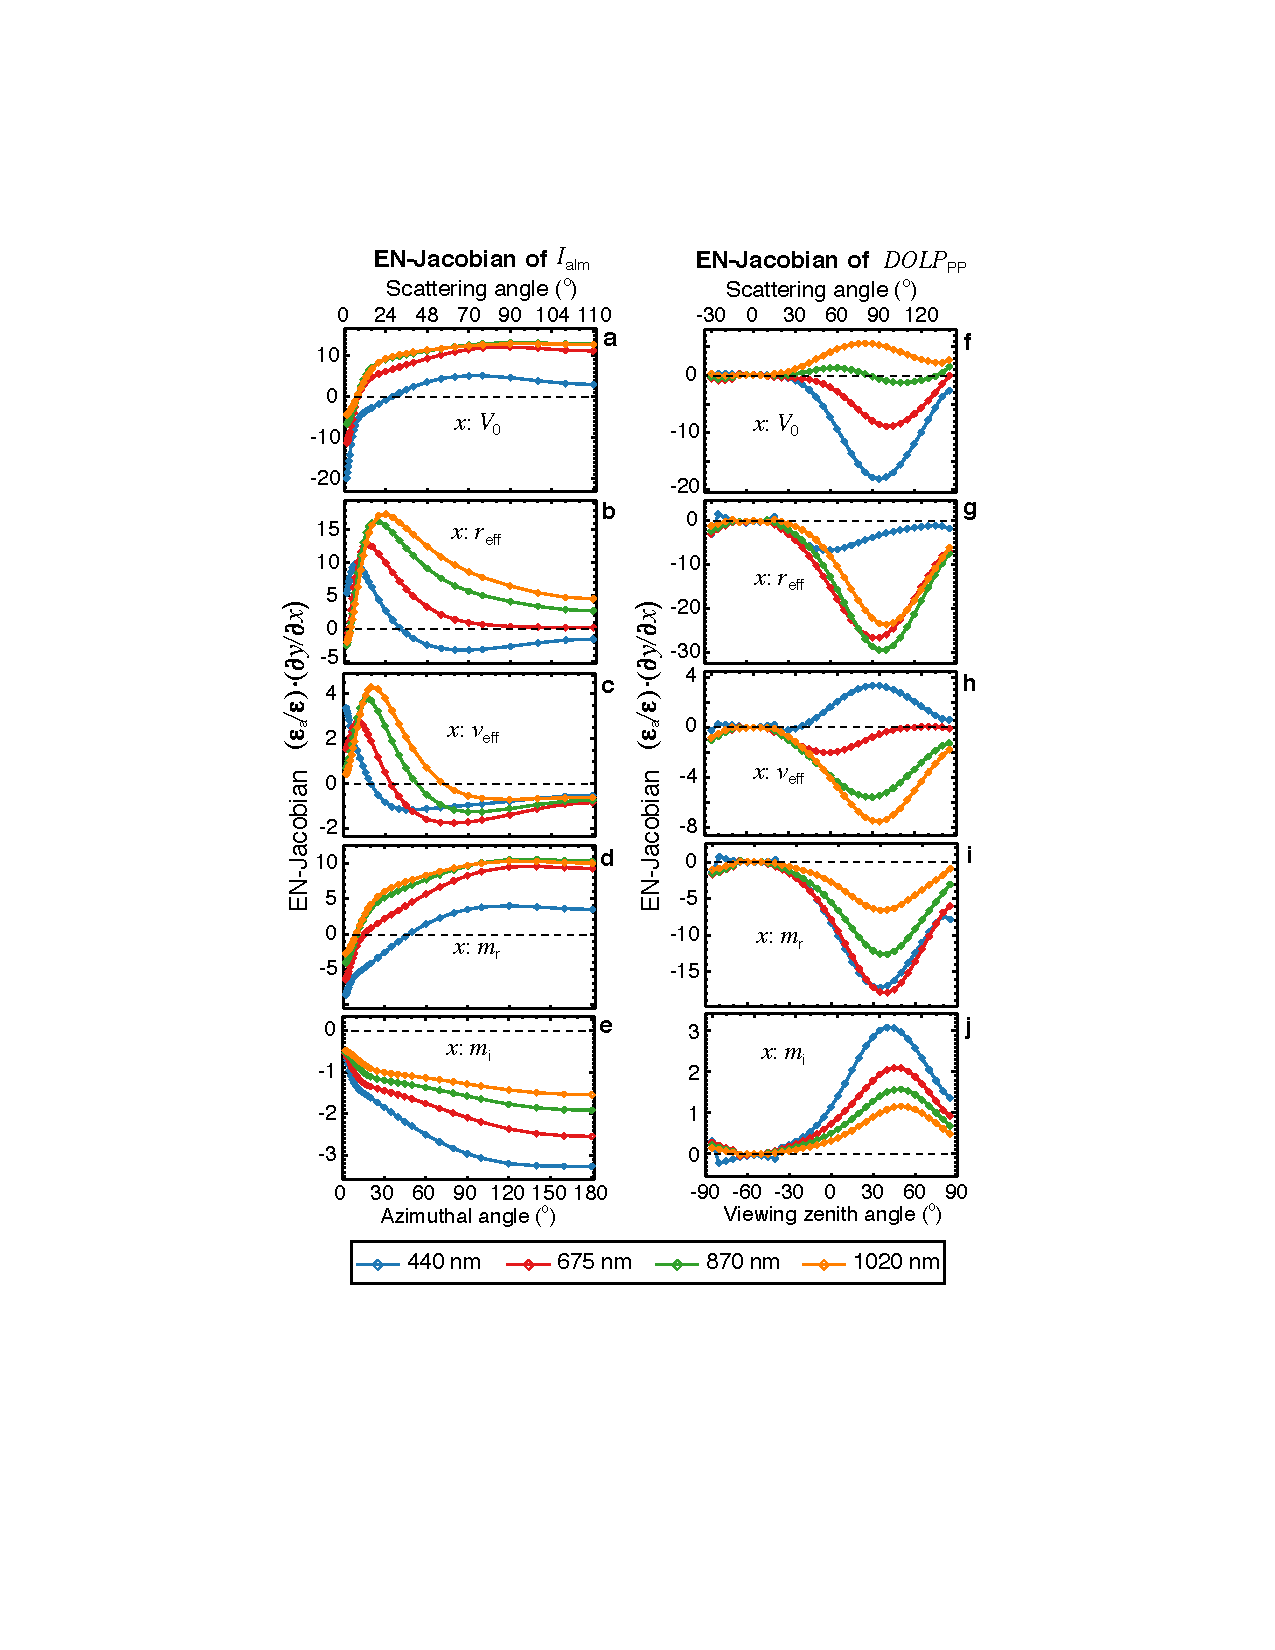
\includegraphics[width={0.8\textwidth}]{figures/info03.pdf}
  \caption{Error-normalized Jacobians of almucantar radiances $\ialm$ (left
column) and degree of linear polarization $\dolppp$ (right column) with respect
to retrieved aerosol parameters in the \textit{fine} mode: (a, f) $V_0$, (b, g)
$\reff$, (c, h) $\veff$, (d, i) $\mreal$, and (e, j) $\mimag$. Simulations use
type-II aerosols with columnar AOD of 1.0 at 440 nm and solar zenith angle of 
55$^\circ$. The top and bottom abscissas are respectively the scattering angle
and SunPhotometer scanning geometries.}
  \label{fig:infoenjf}
\end{figure}

%% Figure EN Jacobian Coarse mode
\begin{figure}[p]
  \centering
  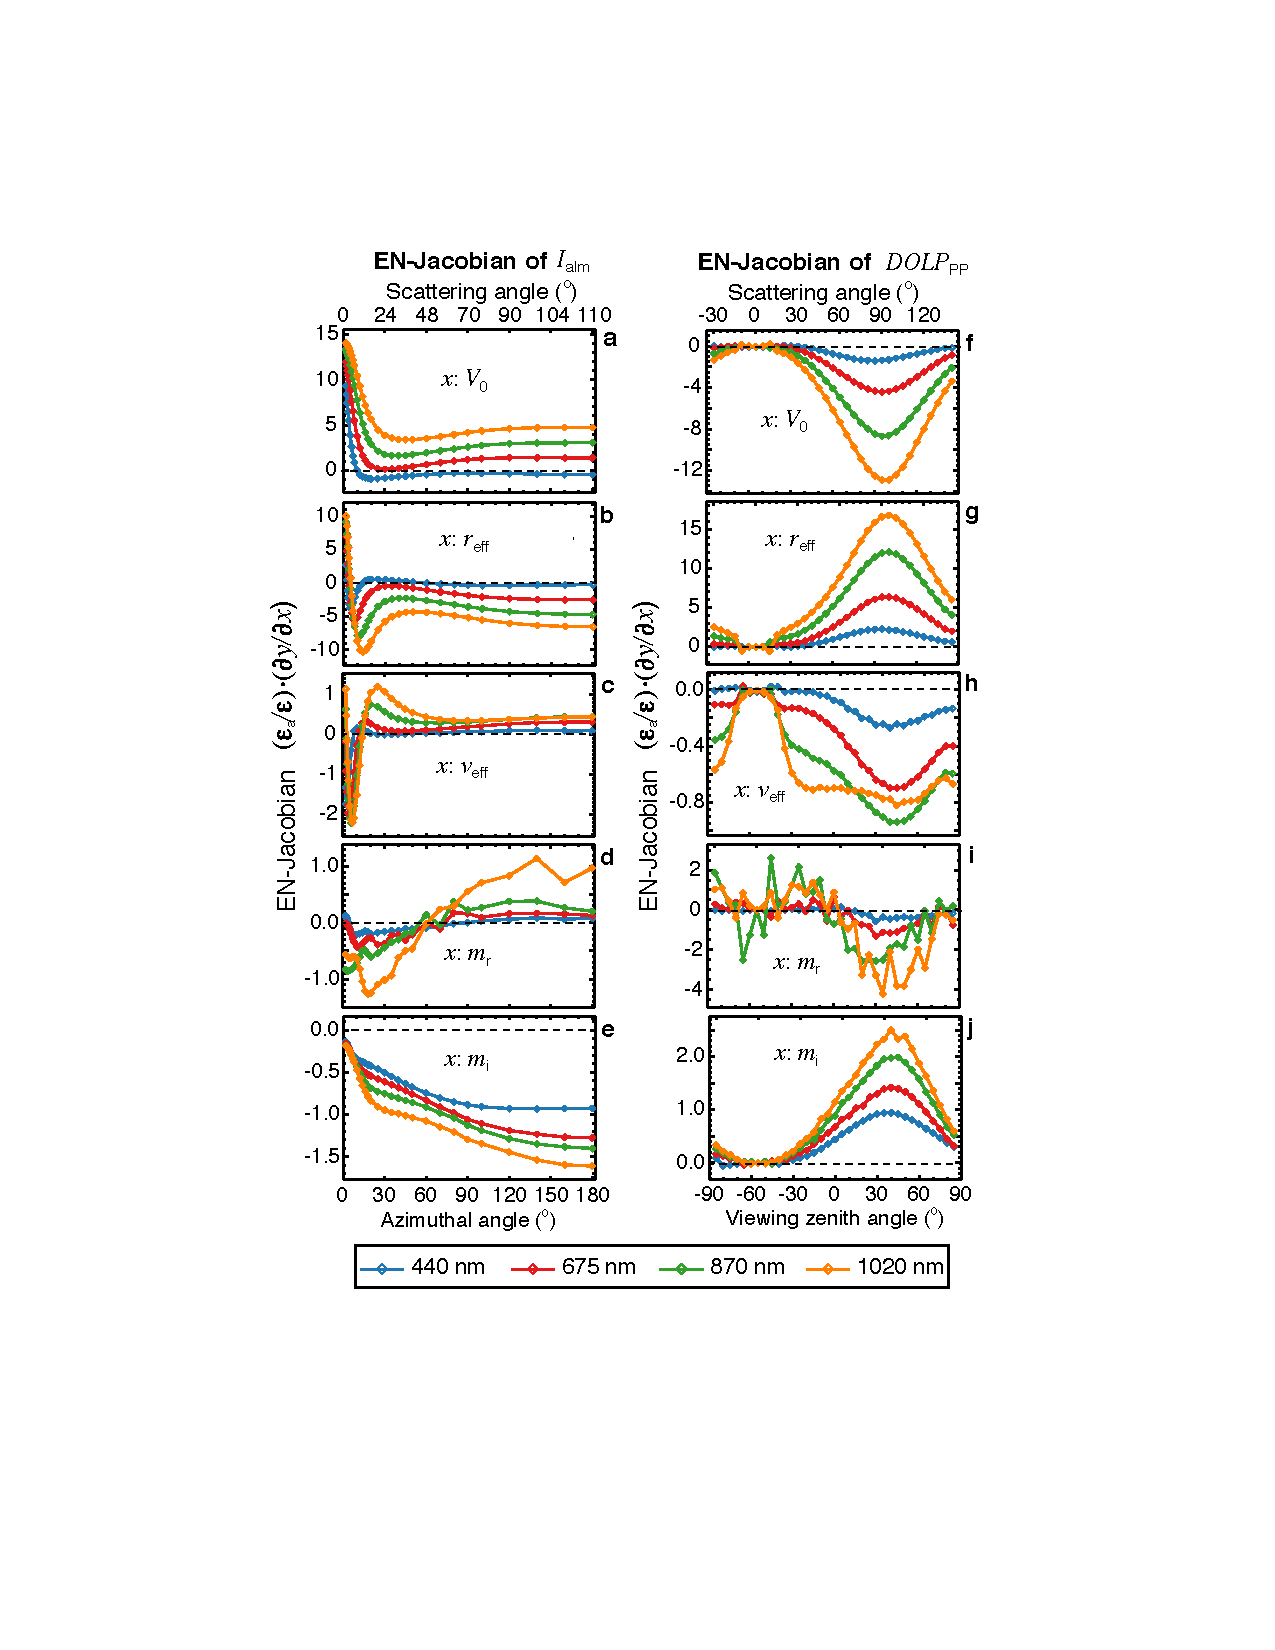
\includegraphics[width={0.8\textwidth}]{figures/info04.pdf}
  \caption{Same as Figure \ref{fig:infoenjf} but for parameters of aerosol in 
the \textit{coarse} mode.}
  \label{fig:infoenjc}
\end{figure}

Furthermore, the EN Jacobians of $\ialm$ and $\dolppp$ can also be synergized 
in terms of their variations on the spectral wavelength. For example, the EN
Jacobians for $\ialm$ with respect to the fine-mode $V_0$ express lowest at 
440 nm (blue curve in Figure \ref{fig:infoenjf}a), but those for $\dolppp$ at 
440 nm (blue curve in Figure \ref{fig:infoenjf}f) are largest ones among these
four spectral bands. Indeed, variations of these sensitivities with wavelength
are mainly determined by the change of size parameter $\eta$, which defined 
as the ratio of the particle size to the applied spectral wavelength, 
$\eta=2\pi\reff/\lambda$. The $\dolppp$ in scattering angles near 90$^\circ$
approaches unity under pure Rayleigh scattering regime where $\eta \ll 1$. 
When the  $\eta$ increases, the value of $\partial\dolppp/\partial{V_0}$ 
decreases and transits into negative at $\eta \sim 2$, reaches negative 
maxima at $\eta \sim 10$, then increases and slowly transits back to positive
when $\eta$ is as large as $\sim 40$ \citep{Hansen74}. The magnitude of the 
$\eta$ at these four bands ranges from 3.0 to 1.3 for the fine-mode particles 
and from 27 to 11 for the coarse-mode particles. Therefore we can understand 
that: (i) the sensitivity of $\dolppp$ to the fine-mode $V_0$ is
positive at 1020 nm due to the small size parameter $\eta=1.3$ (orange curve 
in Figure \ref{fig:infoenjf}f); (ii) this sensitivity gets weaker at 675 nm to
 870 nm and transits to negative at 440 nm as $\eta$ increases 
(Figure \ref{fig:infoenjf}f); and (iii) this sensitivity for aerosol in the 
coarse mode is more negative for longer wavelengths that are
corresponding to smaller values of $\eta$. 

We also note that sensitivity of the $\ialm$ to PSD parameters dominates for
scattering angles less than $\sim$40$^\circ$ (Figures \ref{fig:infoenjf}b-c and 
\ref{fig:infoenjc}b-c), while its sensitivity to $\mreal$ and $\mimag$ 
prevails at larger scattering angles (Figures \ref{fig:infoenjf}d-e and
\ref{fig:infoenjc}d-e). In the near-forward scattering angular regions, the 
dominant scattering effect is the diffraction of light, which essentially 
depends on the size of particles and is independent of the index of refraction
\citep{vandeHulst81, Hansen74}. The $\dolppp$, in contrast, is sensitive to both
the aerosol size and the refractive index at scattering angles from 45$^\circ$ 
to 135$^\circ$ (right columns of the Figures \ref{fig:infoenjf} and
\ref{fig:infoenjc}). Variations of the sensitivity among spectral bands can be
explained by the wavelength-dependent size parameters as discussed in the above
paragraph.  

Overall, the $\dolppp$ EN Jacobians have similar or larger magnitudes to these of
$\ialm$, indicating that the $\dolppp$ measurements possess equal or larger
information for the inversion of these aerosol properties. Adding such
complementary $\dolppp$ measurements to the current radiance-only inversion can
potentially increase the retrieval accuracy. The magnitude of EN Jacobian
elements varies among retrieved parameters, which leads to the variability of
retrieval accuracy. The EN Jacobians with respect to the $V_0$ and $\reff$ of both
modes and the fine-mode $\veff$ and refractive index are larger than those of
other parameters. Correspondingly, these parameters are expected to achieve
higher accuracy in the retrieval. While the maxima in EN Jacobians of $\ialm$
with respect to the coarse-mode refractive index at 870 and 1020 nm slightly
excess unity (Figure \ref{fig:infoenjc}d-e), larger counterparts for $\dolppp$ 
(Figure \ref{fig:infoenjc}i-j) will likely result in improved retrievals. 
In contrast, magnitudes of EN Jacobian for both $\ialm$ and  $\dolppp$ with 
respect to coarse-mode refractive index at 440 and 675 nm are smaller than 
unity across the whole angular range. Adding polarization may not improve the
retrieval for coarse-mode refractive index at those shorter wavelengths in 
such aerosol scenario. However, the consideration of spectral dependence of 
refractive index by using the smoothness constraints will potentially resolve
this problem \citep{Dubovik04}.

\subsection{Information content and retrieval error}

We calculated the averaging kernel matrix $\Abf$, DFS, and \textit{a
posteriori} error for retrieved parameters from these four scenarios of 
observation defined in Table \ref{tab:infoy}. Figuress \ref{fig:infodfs1}a-c 
illustrate how the DFS varies with the solar zenith angles for
three defined aerosol types. The DFS in the scenario I2 (red curves) ranges
from 14 to 15 for the fine-dominated aerosol model, and from 17 to 19 for other
two aerosol models, about 2–3 degrees higher than those using AODs and $\ialm$
measurements in the scenario I1 (black curves), indicating that sky radiances
in the principal plane ($\ipp$) contain additional information. The scenario P1
(green curves), which comprises solar almucantar sky radiances and
principal-plane polarimetric radiances at four wavelengths, further increases
DFS by 1–2. Observations in the scenario P2 (blue curves)—radiance and
polarization in the almucantar plane—yields DFS values slightly below those in
the scenarios I2 and P1. Therefore, from Figure \ref{fig:infodfs1} we conclude
that adding measurements in the solar principal plane into the inversion 
significantly increases the information content for aerosol properties, 
especially when combining the $\ipp$ and $\dolppp$. We also note that the 
DFS increases with solar zenith angle for all cases. Observations in larger 
solar zenith angle enable a wider range of scattering angles (Figure
\ref{fig:infodfs1}d), and thus contain more information
on the aerosol scattering phase function and in turn on the aerosol
microphysical parameters.

%% Figure DFS vs theta
\begin{figure}[t]
  \centering
  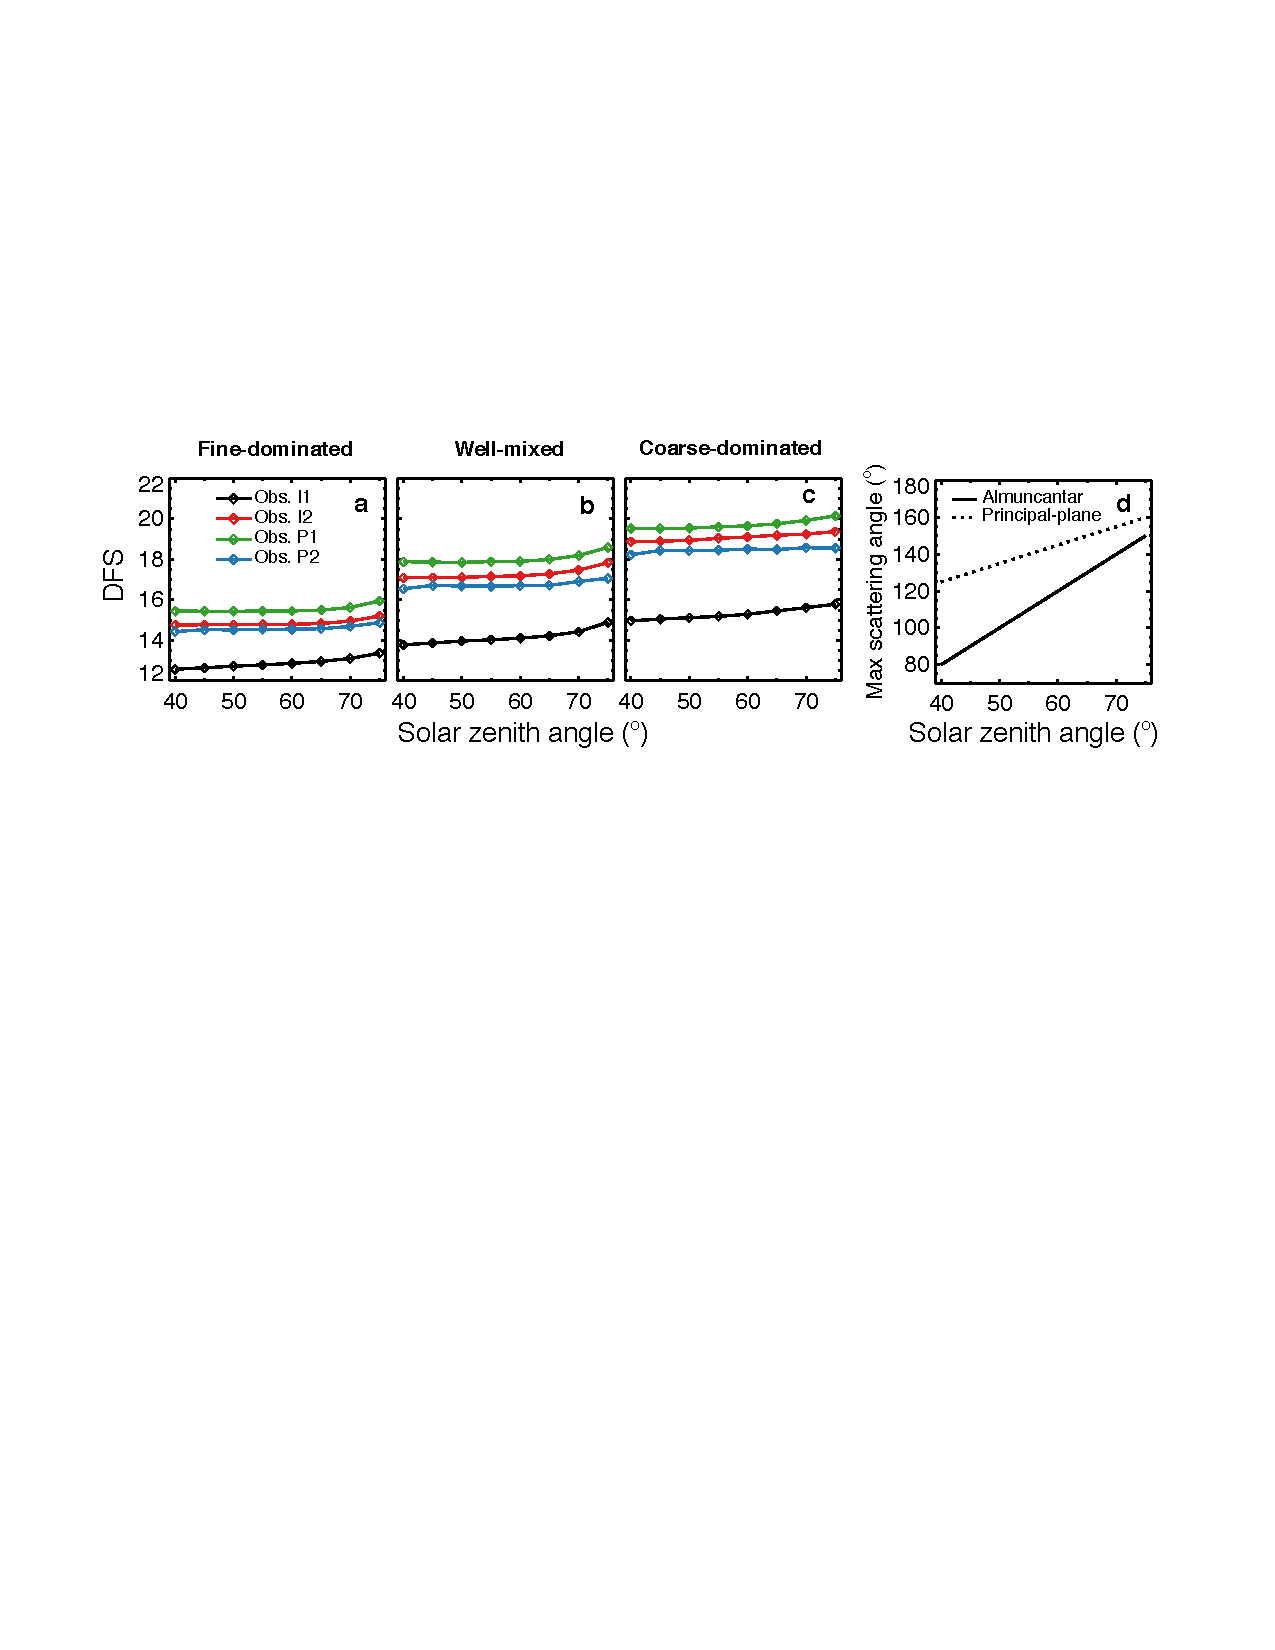
\includegraphics[width={\textwidth}]{figures/info05.pdf}
  \caption{Degree of freedom for signal (DFS) as a function of solar zenith
angle for retrieving all 22 parameters when using aerosol type of (a)
fine-dominated,  (b) well-mixed, and (c) coarse-dominated. Four differently
colored-curves denote four observation scenarios defined in Table 1. Panel (d)
shows the maximum scattering angles that can be reached by the almucantar and
the principal-plane scans.}
  \label{fig:infodfs1}
\end{figure}

We illustrate the DFS components $\Abf_{i,i}$ in Figure \ref{fig:infodfspsd1} 
for the $V_0$, $\reff$ and $\veff$, and in Figure \ref{fig:infodfsmr} and
\ref{fig:infodfsmi} for the $\mreal$ and $\mimag$, respectively. Also shown
in those figures are the a posteriori errors, which are the diagonal elements
of $\hat{\Sbf}^{\frac{1}{2}}$. It should be noted that errors for $V_0$,
$\reff$, and $\veff$ are in terms of relative uncertainties (\%), while errors
in the $\mreal$ and $\mimag$ are absolute quantities. Curves of four different
colors in each panel indicate these defined four observation scenarios and
are averages for the three aerosol types. Error bars represent one fifth of 
the standard deviations among the three aerosol types (the use of the o
ne-fifth scale is only for plotting purpose). These error bars thus depict
the variability of the DFS component and retrieval error over the fine-mode 
fraction ($\fmfv$). Mean retrieval uncertainties averaged over various solar 
zenith angles are summarized in Table \ref{tab:infoerr}. We discuss these results 
for each retrieved parameter in detail as following. 

\subsubsection{Aerosol PSD}

Among the 22 elements in the state vector, the $V_0$, $\reff$ and $\veff$ 
describe the aerosol PSD. According to Figure \ref{fig:infodfspsd1}a-c, 
observations in the scenario P1 (green curves) always yield the highest 
DFS components for inferring PSD parameters in both the fine and coarse modes,
followed by observations from the scenarios I2 (red) and P2 (blue), and lastly
the scenario I1 (black). As a consequence, the \textit{a posterior} errors are
found smallest for the scenario P1 and largest for the scenario I1 (Figure 
\ref{fig:infodfspsd1}d-e). Retrieval errors in the scenario I1 (black curves)
are 5--15\% for $V_0$, 5--9\% for $\reff$, and 20--30\% for $\veff$,
which vary with solar zenith angles. In contrast, retrieval errors in the
scenario P1 (green curves) are reduced to $\sim$2.5\%(3\%), 1\%(3.5\%), and 
7\%(20\%) for the fine (coarse) mode. From observations in the scenarios P2
and I2, one can retrieve $V_0$, $\reff$, and $\veff$ of errors lying between
the scenarios I1 and P1, though slightly larger in the scenario P2. 
In addition, higher DFS components and smaller retrieval errors are found for
the fine-mode parameters than those for the coarse mode, because radiances
and polarization are in particular more sensitive to aerosol parameters in the
fine mode as shown in the contrast between the Figures \ref{fig:infoenjf} and 
\ref{fig:infoenjc}

%% Figure DFS and error of PSD 
\begin{figure}[t]
  \centering
  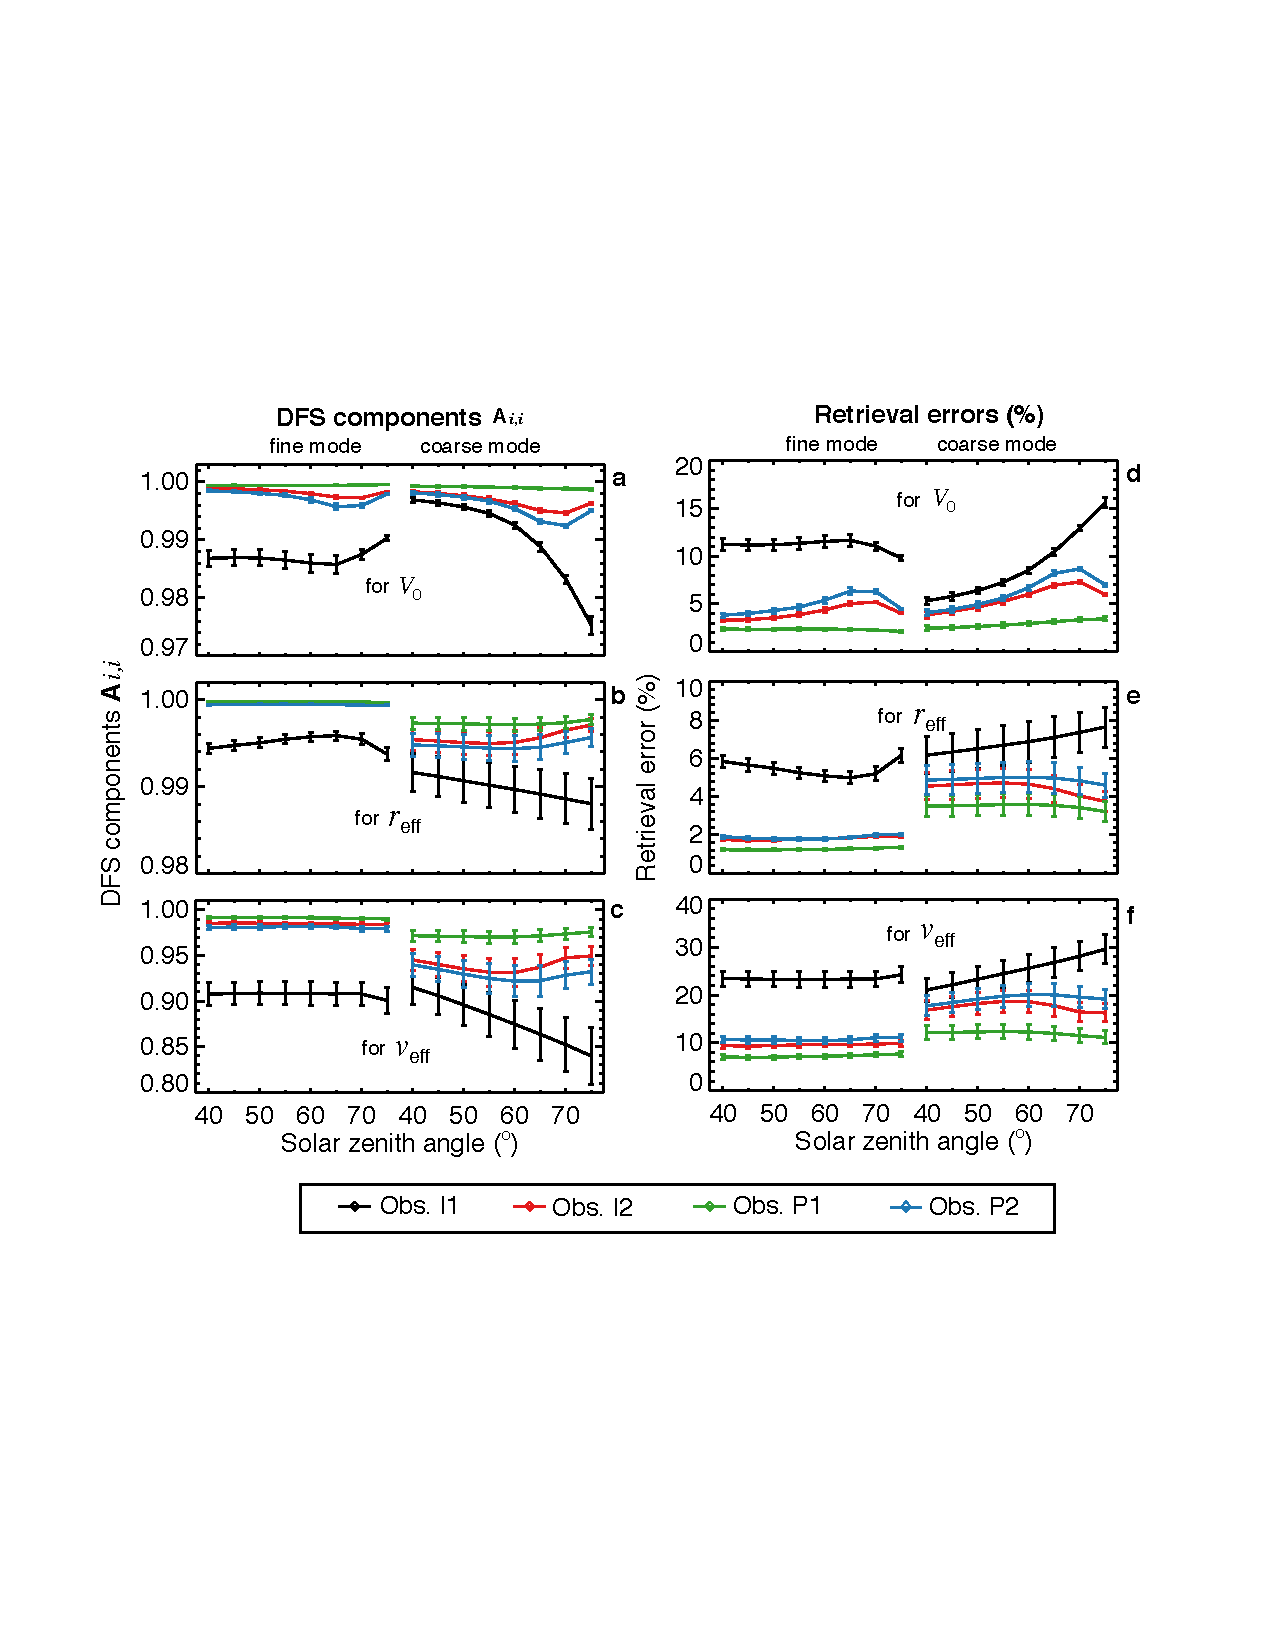
\includegraphics[width={\textwidth}]{figures/info06.pdf}
  \caption{DFS components (left column) and retrieval uncertainty (right
column) as a function solar zenith angle with different observation scenarios
defined in Table \ref{tab:infoy}. Quantities are averages for three aerosol 
types defined in Table \ref{tab:infoopt}, and error bars represent 
one fifth of standard deviation. Three rows from top to bottom are 
respectively for retrieving $V_0$, $\reff$, and $\veff$. In
each panel, shown in the left is for the fine mode and in the right is for the
coarse mode.}
  \label{fig:infodfspsd1}
\end{figure}

We also note that, in the scenario I1, DFS components for the coarse-mode
parameters decrease with increasing solar zenith angle, while no obvious trend
can be found for the fine-mode parameters. This can be explained by the low
sensitivity of the $\ialm$ to the coarse-mode $V_0$, $\reff$, and $\veff$ at
large scattering angles as showed in Figure \ref{fig:infoenjc}a-c. Higher 
sensitivities occur at scattering angles below $\sim$30$^\circ$; the increase
in SZA results in a smaller number of measurements in the near-forward 
scattering angular regions, and thus leads to larger retrieval errors. 
However, these trends turn to be weaker or negligible in other observation 
scenarios, especially the scenario P1. We can understand this from two aspects.
First, observations from principal plane can add additional measurements near
the forward scattering region. Second and most importantly, the added 
polarization measurements in the scenarios P1 and P2 contain additional 
information that is independent of the scattering angle limitation as 
discussed in the section \ref{subsec:enj}.

Overall, the increase in DFS components by adding polarization measurements is
less than 0.1 for retrieving $V_0$, $\reff$, and $\veff$, because radiances alone
contain abundant information. The retrieval accuracy in aerosol PSD from
observations of all scenarios exceeds the requirements for better quantifying
aerosol climate radiative forcing identified by \citet{Mishchenko04}. Even
so, the addition of multi-band $\dolppp$ measurements to the inversion can
still yield up to $\sim$70\% retrieval error reduction in the fine-mode and up
to $\sim$50\% reduction in the coarse-mode aerosol PSD parameters. 

\subsubsection{Refractive indices}

As shown in Figure \ref{fig:infodfsmr}a-b, different magnitudes prevail in
the DFS components for the $\mreal$ between fine and coarse modes and among
different observation scenarios. For example, DFS components for aerosols in
the fine mode overreach 0.8 at all four wavelengths in the scenario I1; while
the counterparts in the coarse mode approach 0.5 at 1020 nm and are less than
0.2 for the other three wavelengths. This is due to the weaker sensitivity of
almucantar radiances to the coarse-mode $\mreal$  (as in Figure
\ref{fig:infoenjc}d) comparing to that for aerosol in the fine
mode (as in Figure \ref{fig:infoenjf}d). In general, adding the $\dolpalm$,
$\ipp$, or both the $\ipp$ and $\dolppp$ in the inversion increases the DFS
components for $\mreal$ of aerosols in both the fine and the coarse modes. 
Particularly, DFS components achieve the most significant rise in the scenario
P1 by climbing to 0.95--1.0 in the fine mode and to 0.4--0.8 in the coarse 
mode. Also shown in Figure \ref{fig:infodfsmr}a, an increasing pattern with
solar zenith angles is found in the DFS components for the fine-mode aerosol
at larger wavelengths because stronger sensitivity occurs in larger scattering
angles.

%% Figure DFS and error of mr
\begin{figure}[p]
  \centering
  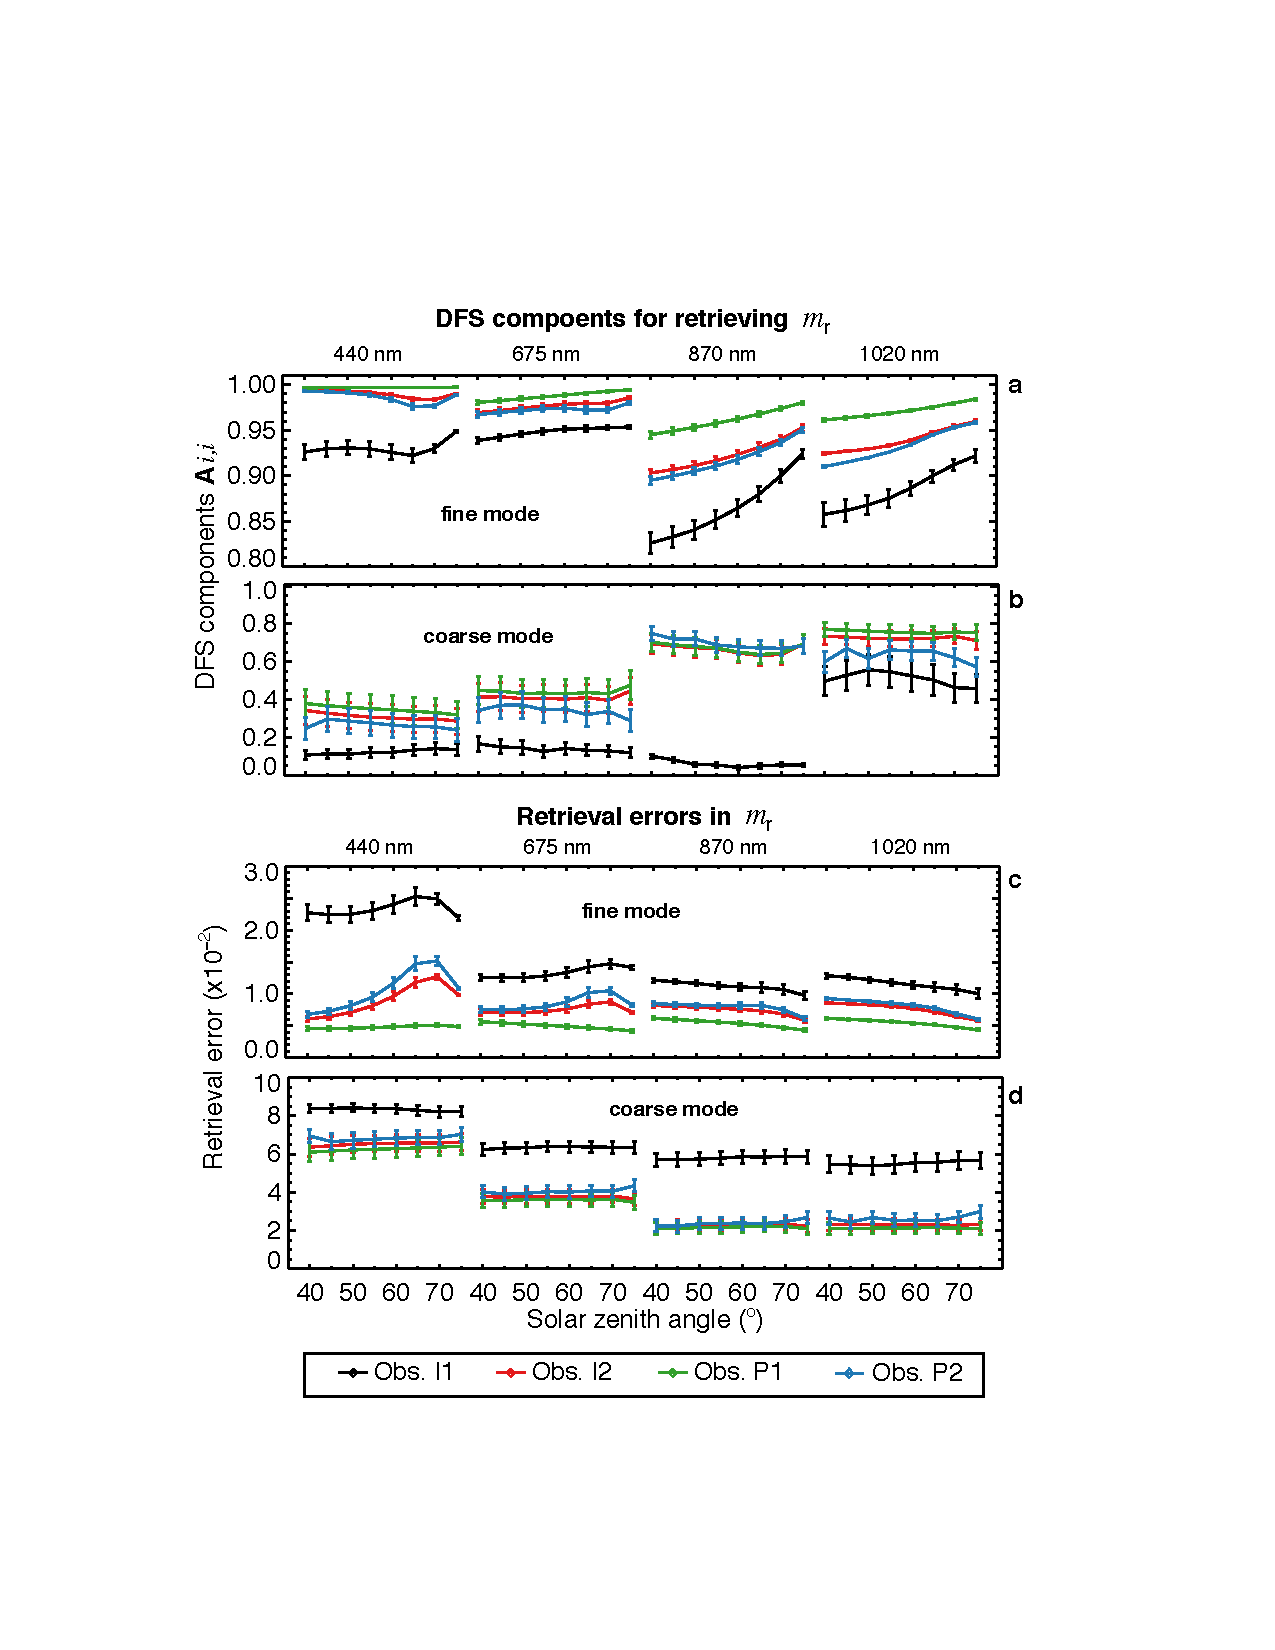
\includegraphics[width={0.9\textwidth}]{figures/info07.pdf}
  \caption{Same as Figure \ref{fig:infodfspsd1} but for DFS components (a-b) and 
retrieval uncertainty (c-d) for retrieving real part refractive index $mreal$ 
in four wavelength bands. (a) and (c) are for the fine aerosol mode, while 
(b) and (d) for the coarse mode. }
  \label{fig:infodfsmr}
\end{figure}

%% Figure DFS and error of mi
\begin{figure}[p]
  \centering
  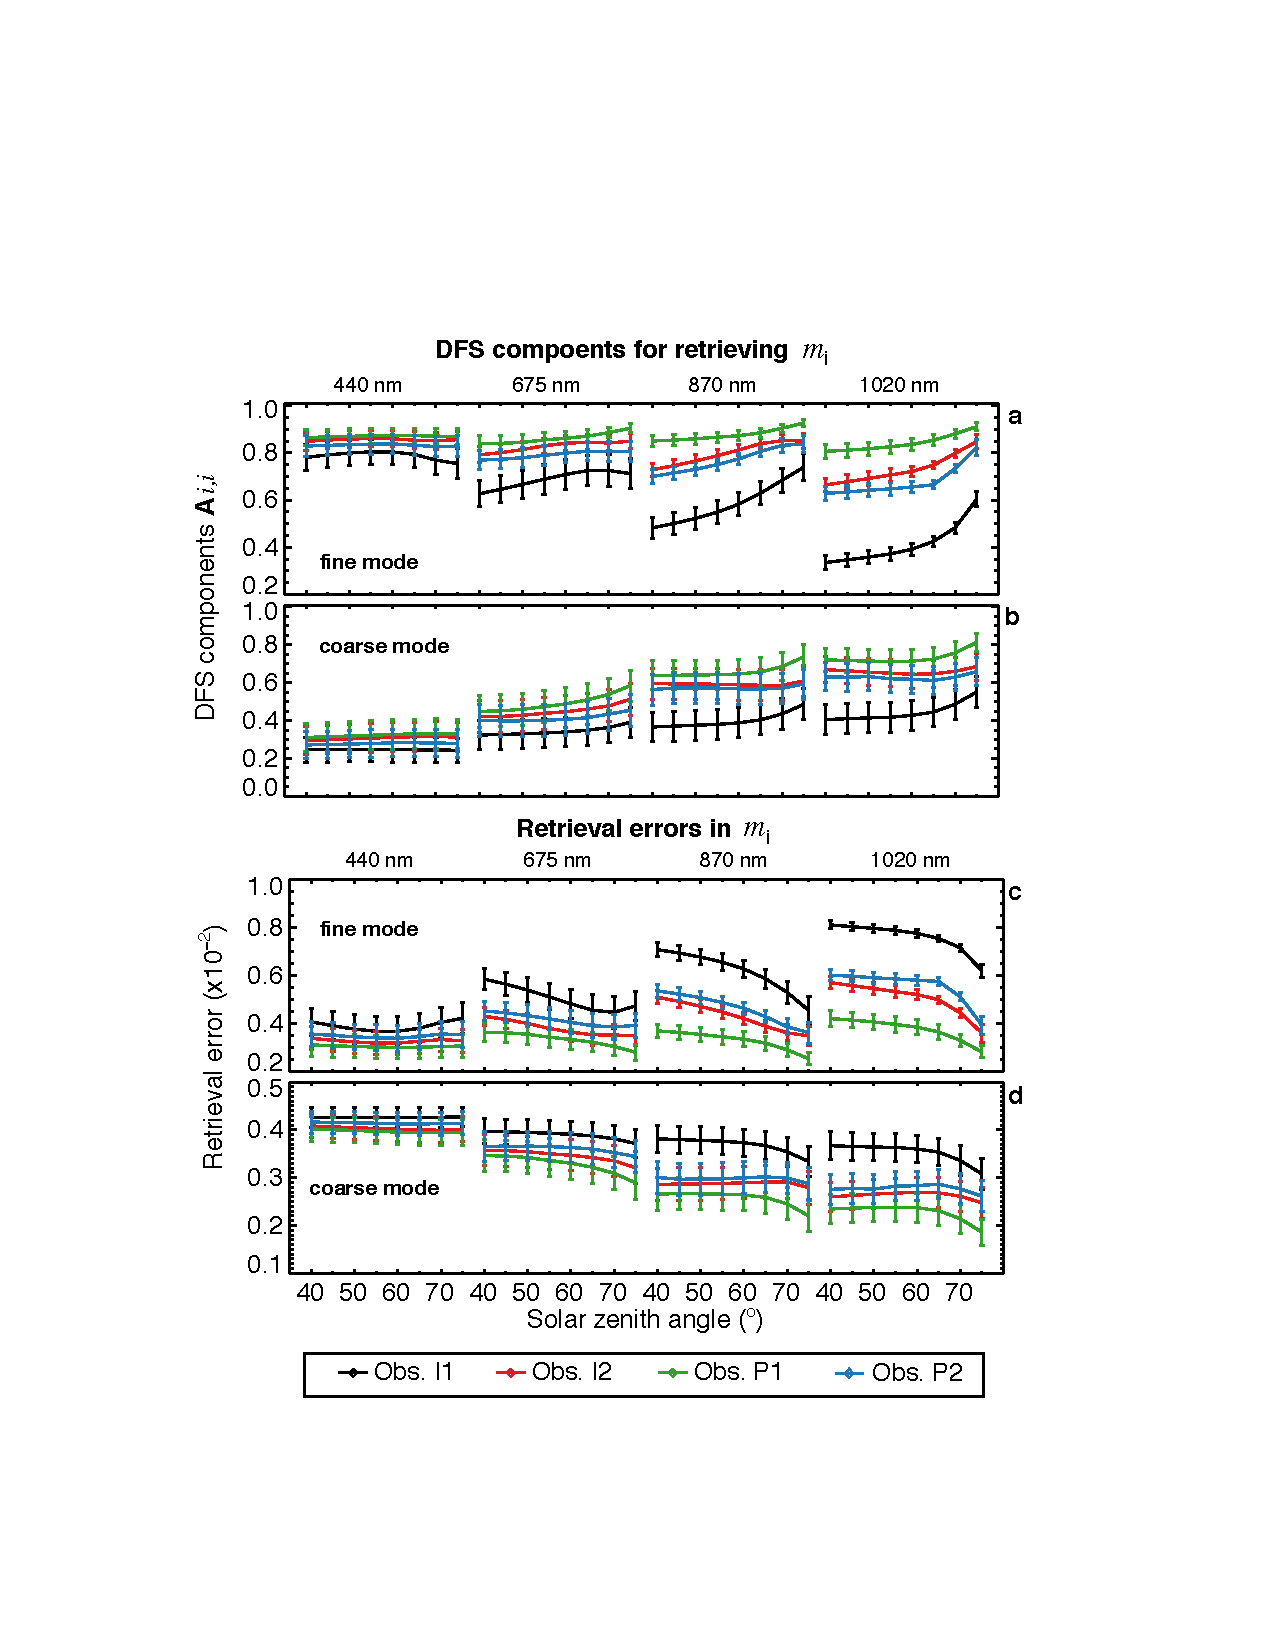
\includegraphics[width={0.9\textwidth}]{figures/info08.pdf}
  \caption{Same as Figure \ref{fig:infodfsmr} but for retrieving imaginary 
part refractive index $\mimag$.}
  \label{fig:infodfsmi}
\end{figure}

As expected, the retrieval of $\mreal$ can be more accurate by adding additional
measurements. According to Figure \ref{fig:infodfsmr}c-d, the \textit{a
posteriori} error in $\mreal$ averaged on the four spectral bands is 
$\sim$0.015 (0.065) for aerosols in the fine (coarse) mode from measurements
in the scenario I1. In contrast, it is reduced to 0.008 (0.037), 0.005 (0.035), 
and 0.009 (0.040) in the scenarios I2, P1, and P2, respectively. 
Retrieval errors in the coarse-mode $\mreal$ are larger in shorter
spectral wavelengths because of weaker sensitivity to the $\ialm$ and DOLP. 
For instance of the scenario P1, it is about 0.06 at 440 nm, 0.035 at 675 nm, 
and 0.02 at 870 and 1020 nm. 

The DFS components for the $\mimag$ are shown in Figure \ref{fig:infodfsmi}a–b,
and the corresponding retrieval errors in $\mimag$ are displayed in 
Figure \ref{fig:infodfsmi}c–d. Similar to those for the $\mimag$, DFS
components for retrieving the $\mimag$ are larger in the fine mode and show
an increasing pattern with the solar zenith angle. Observations in the scenario
P1 always yield largest DFS components and smallest retrieval error for the
$\mimag$, followed by the scenarios P2 and I2. Observations in the scenario I1
offer the $\mimag$ retrieval with largest error. If averaged on the solar
zenith angles and aerosol types, the retrieval error in the $\mimag$ is 
0.006 (0.004) for aerosol in the fine (coarse) mode in the scenario I1, and 
can be reduced to 0.003 (0.003) in the scenario P1. 

%% Table of retrieval error 
\begin{table}[t]
  \centering
  \small
  \caption{Error for retrieved and derived parameters among \textit{a priori},
          \textit{a posteriori}, and Glory characterization\textsuperscript{a}.}
  \label{tab:infoerr}
  \begin{tabular}{p{4em} C{4em} C{4em} C{4em} C{5em} C{5em} C{5em} }
  \toprule
  & \multicolumn{5}{c}{Error in retrieved parameters} \\
  \cmidrule(r){2-6} 
  Entries & $V_0$ (\%)& $\reff$ (\%)& $\veff$ (\%)& $\mreal$ & $\mimag$ & $\assa$ \\
  \midrule
   A priori & 100/100 & 80/80 & 80/80& .15/.15 & .01/.05 & - \\
   Obs. I1 & 11./9.0 & 5.5/6.8 & 23/25 & .015/.065 & .0057/.0038 & .037/.085 \\
   Obs. I2 & 4.1/5.5 & 1.8/4.4 & 10/18 & .008/.037 & .0041/.0032 & .024/.073 \\
   Obs. P1 & 2.3/2.9 & 1.3/3.5 &7.2/12 & .005/.035 & .0033/.0030 & .019/.068 \\
   Obs. P2 & 4.9/6.2 & 1.9/4.9 & 11/19 & .009/.040 & .0044/.0034 & .026/.076 \\
   Glory$^b$ & –     & 10 & 40 & .02  & – & .03 \\
  \bottomrule
  \multicolumn{7}{m{35em}}{\textsuperscript{a}Results of our work are averaged
values for three aerosol types and for solar zenith angles from 
40$^\circ$ to 70$^\circ$. \newline \textsuperscript{b}Referred to
\citet{Mishchenko04}.}  
  \end{tabular}
\end{table}

\subsubsection{Single scattering albedo}

Note that the aerosol single scattering albedo $\assa$ is an intermediate rather
than a directly retrieved parameter. The error in $\assa$ can be estimated
from the $\hat{\Sbf}$ with the equation \eqref{eq:zeta}. The $\assa$ for each
aerosol mode uniquely depends on the light wavelength and aerosol 
microphysical parameters including $\reff$, $\veff$, and $\mreal$ and $\mimag$,
although the $\mimag$ impacts $\assa$ most significantly \citep{Hansen74}.
Required derivatives of $\assa$ to these parameters in the equation
\eqref{eq:zeta} can be obtained from the linearized Mie code (section
\ref{subsec:mie}) integrated into the UNL-VRTM. We calculated uncertainties 
in the $\assa$ for each wavelength and each aerosol type, and the averaged 
values are summarized in Table \ref{tab:infoerr}. Observations in these four 
scenarios can  retrieve $\assa$ with the uncertainty of 0.037, 0.024, 0.019, 
and 0.026 for  the fine mode, and 0.085, 0.073, 0.068, and 0.076 for the coarse
mode, respectively. Thus, only the fine-mode $\assa$ retrieval with polarization
involved can meet the accuracy requirements (0.03) for accurate climate forcing
estimates \citep{Mishchenko04}. We noted that the mean uncertainty in the
coarse-mode $\assa$ exceeds 0.06 in all of these four scenarios, but higher
accuracy may be achieved under coarse-dominated conditions as shown in the
following section.  

\section{Sensitivity of retrieval error to AOD and fmf} \label{sec:infosensi}

The performance of retrieval usually varies with aerosol conditions like
the aerosol loading and the prevalence of aerosol in either the fine or
the coarse modes (e.g., fine-mode volume fraction, $\fmfv$). As a result,
uncertainties in aerosol retrievals can depend much more strongly on the
AOD than they do on the properties of an individual aerosol model
\citep{Knobelspiesse12}. For the same reason, the inversion of
refractive indices and $\assa$ in the current AERONET algorithm is confined
to the condition when the 440-nm AOD is larger than 0.4
\citep{Dubovik00b, Holben06}. Our above analysis, which focused on three
aerosol types by a constant AOD value at 440 nm (${\taua}_{440}$=1.0), is
insufficient to represent variable global conditions. At the same time,
we also found noticeable variability of the DFS components and a
posteriori errors existing among three aerosol types with different
$\fmfv$, especially for the coarse-mode parameters. Thus, it is necessary
to investigate how aerosol conditions affect the retrieval error, in
order to answer the question: under what aerosol conditions the AERONET
measurements (with and without polarization) are capable to yield
retrievals with satisfied accuracy?

%% Figure DFS in sensitivity
\begin{figure}[t]
  \centering
  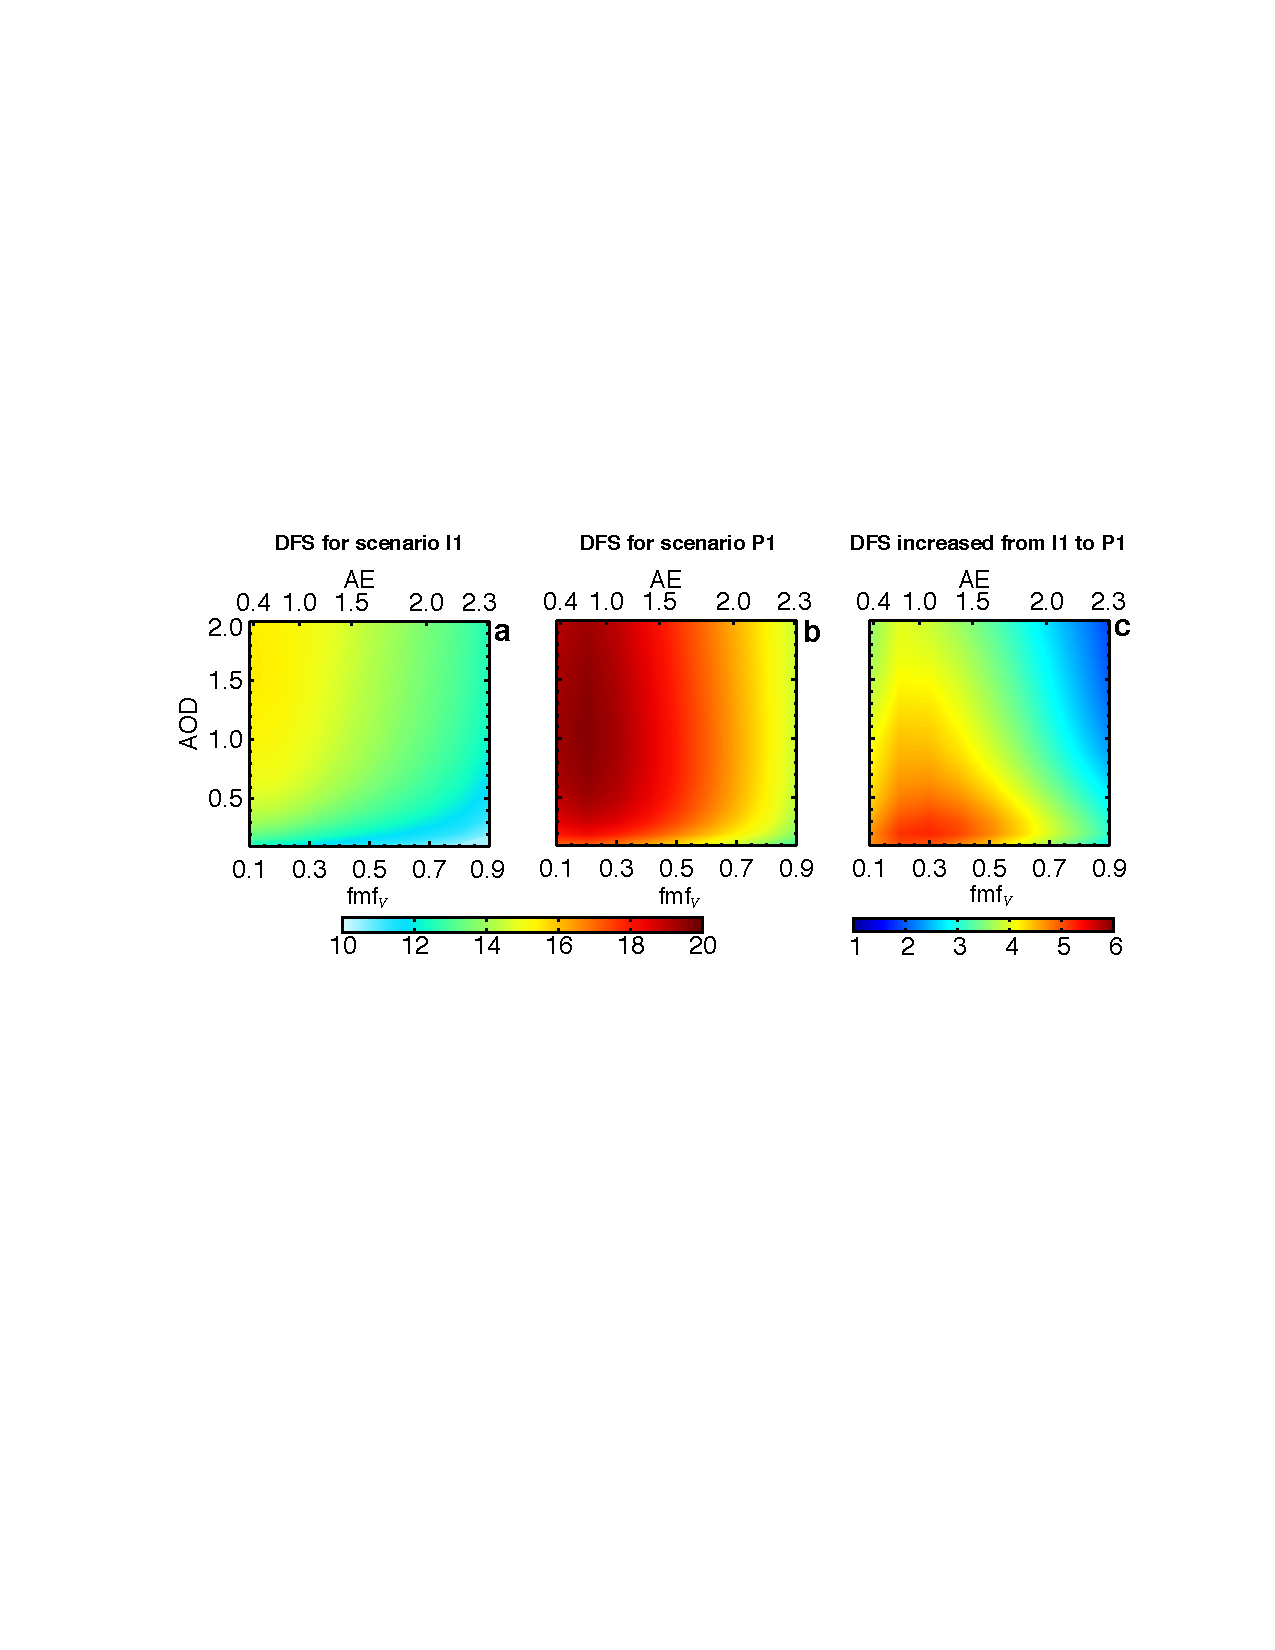
\includegraphics[width={\textwidth}]{figures/info09.pdf}
  \caption{Contours of DFS as a function of $\fmfv$ and AOD in scenarios
I1 (a) and P1 (b). (c) the difference of DFS between (a) and (b).
Simulations are for solar zenith angle of 55$^\circ$. The top abscissa denotes
Ångström exponent (AE).}
  \label{fig:infodfs2}
\end{figure}

We expand our analysis for the ${\taua}_{440}$ ranging from 0.1 to 2.0 
and for the $\fmfv$ from 0.1 to 0.9. In practice, the $\fmfv$ is 
inaccessible prior to inversion. Instead, we use the 
Ångström exponent (AE) from 870 to 1020 nm together with
${\taua}_{440}$ to define the aerosol conditions, because the AE
in the longer paired wavelength is highly related to the $\fmfv$
\citep{Schuster06} and immediately available from the AERONET direct sun 
measurements. With the aerosol properties defined in the Table
\ref{tab:infoy},the $\fmfv$ from 0.1 to 0.9 gives AE values from
0.35 to 2.3. We exclude the scenarios of I2 and P2 in our following
analysis, because the scenario P1 demonstrates the most superior
performance and is also the focus of our algorithm development.

%% Figure error fine-mode in sensitivity
\begin{figure}[p]
  \centering
  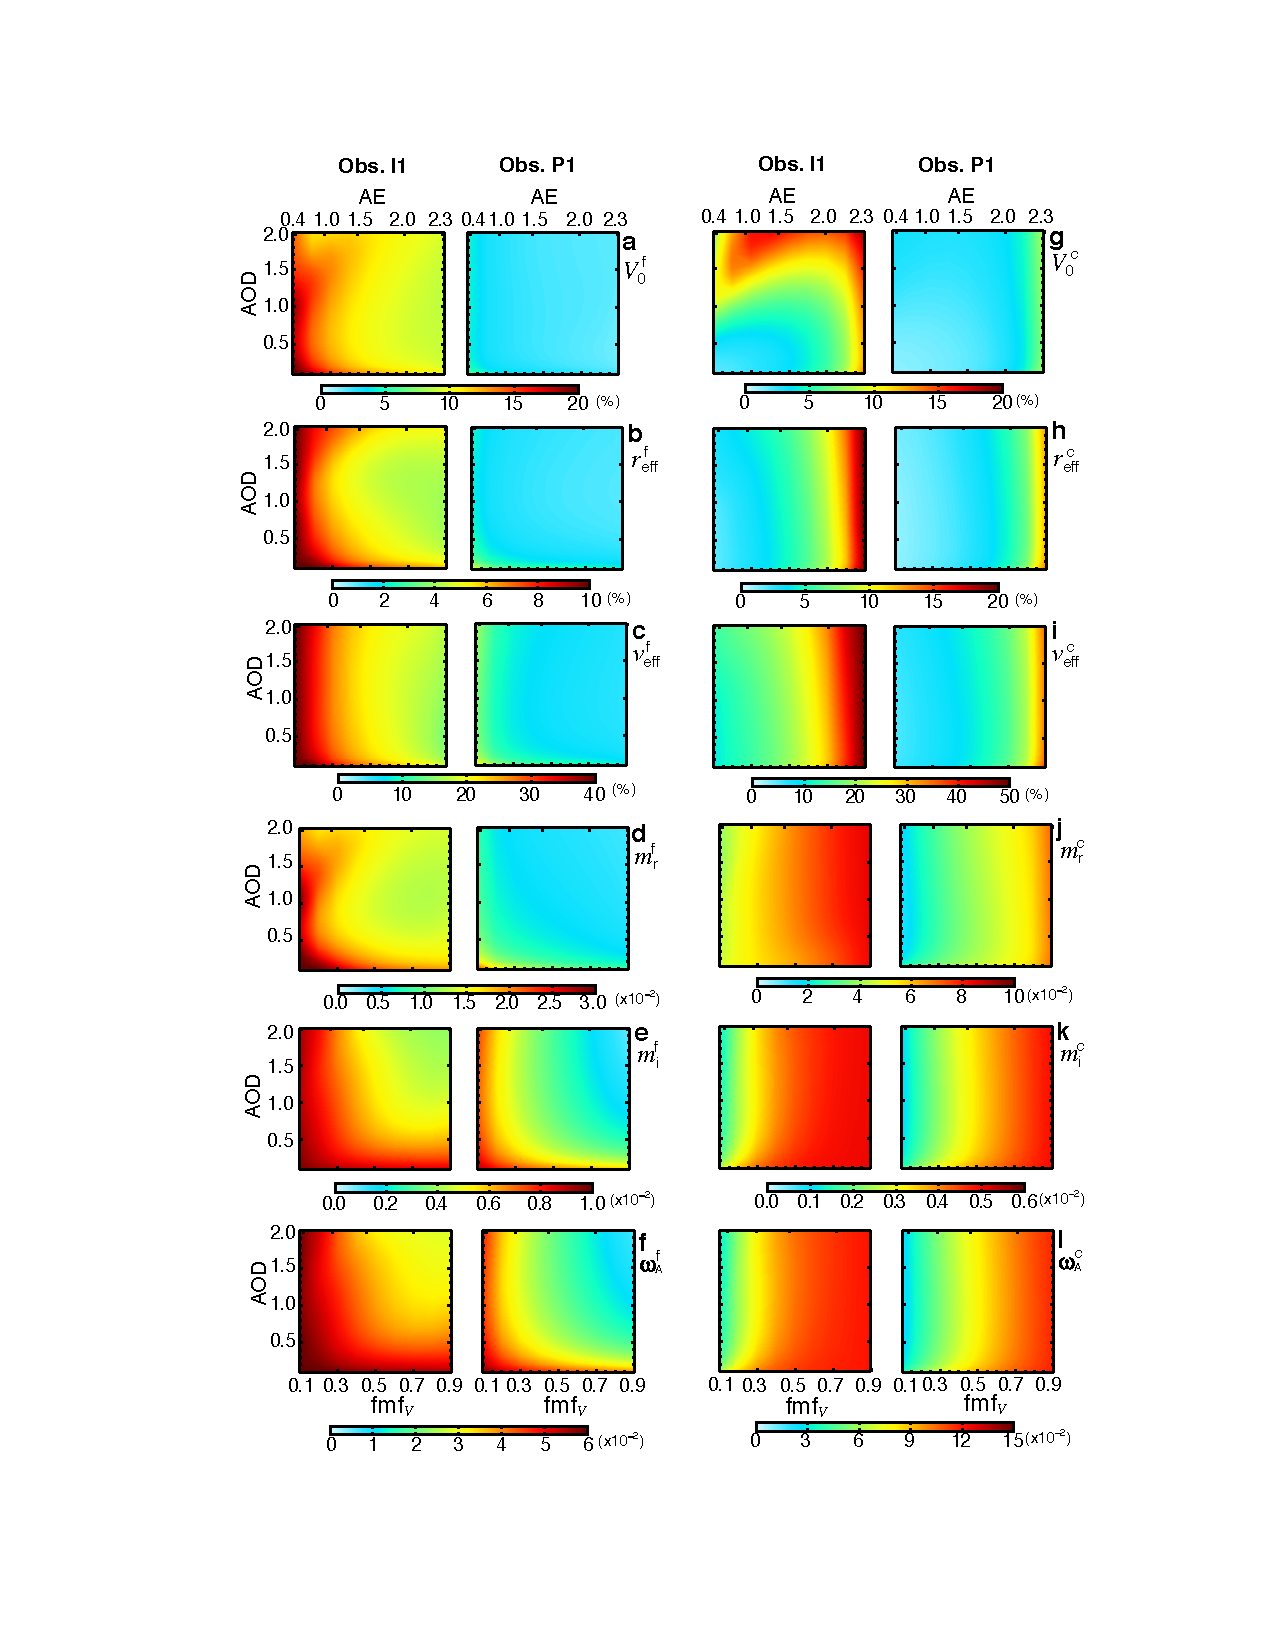
\includegraphics[width={\textwidth}]{figures/info10.pdf}
  \caption{Retrieval uncertainties as a function of $\fmfv$ (or AE) and
AOD for each individual aerosol parameters in the \textit{fine} mode: (a) $V_0$,
(b) $\reff$, (c) $\veff$, (d) $\mreal$, (e) $\mimag$, and (f) $\assa$.
Two sub-panels in each panel indicate observations in the scenarios 
I1 and P1, respectively. Simulations are for solar zenith angle of
55$^\circ$. The x- and y-axis are identical to those in Figure
\ref{fig:infodfs2}. Relative uncertainties are shown for
$V_0$, $\reff$ and $\veff$, while absolute errors for $\mreal$, $\mimag$, 
and $\assa$. Retrieval errors for $\mreal$, $\mimag$, 
and $\assa$ are averaged values over the four spectral bands.}
  \label{fig:infoerrf}
\end{figure}

%% Figure error coarse-mode in sensitivity
\begin{figure}[p]
  \centering
  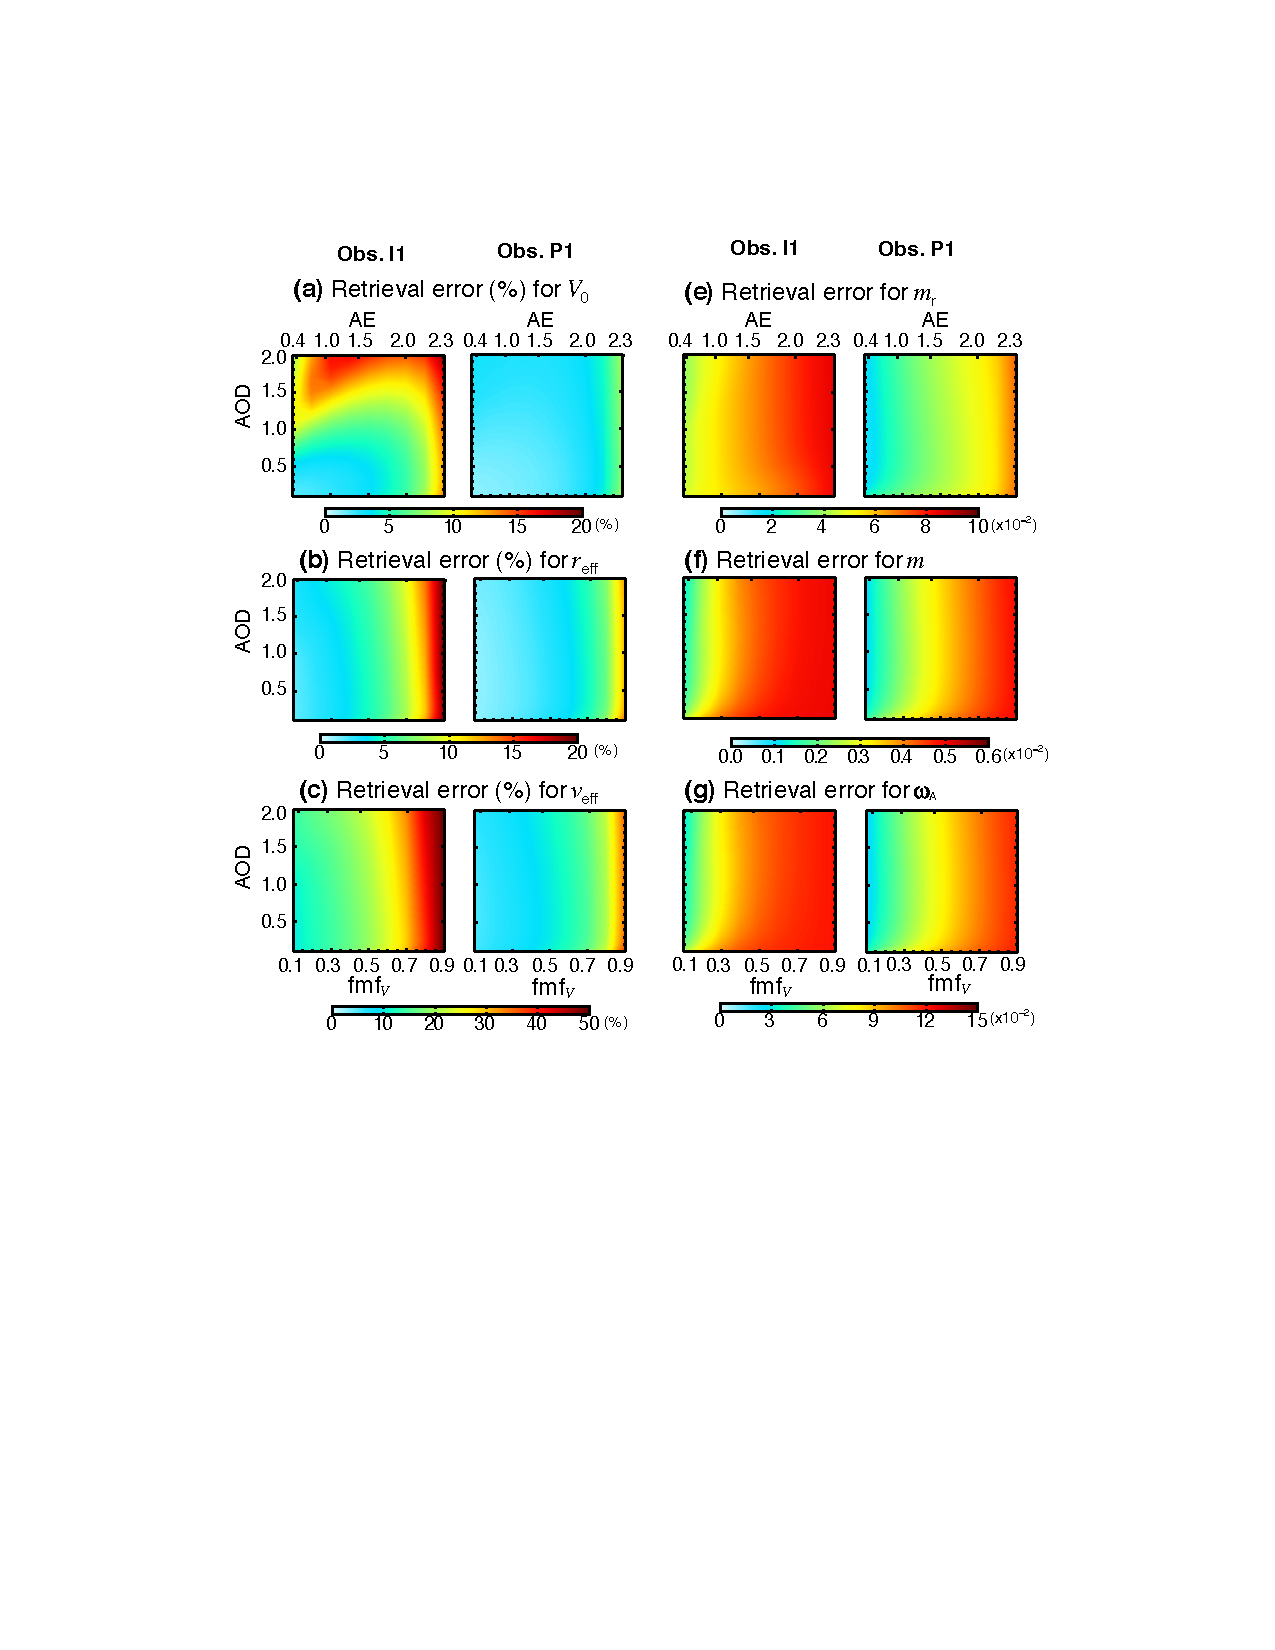
\includegraphics[width={\textwidth}]{figures/info11.pdf}
  \caption{Same as Figure \ref{fig:infoerrf}, but for aerosol parameters in 
the \textit{coarse} mode.}
  \label{fig:infoerrc}
\end{figure}

Figure \ref{fig:infodfs2}a--b display the contours of DFS as a function 
of the AE (or $\fmfv$) and ${\taua}_{440}$ in the scenarios I1 and P1, 
respectively. We found that the DFS decreases with an increasing AE and
$\fmfv$ for the same AOD. This is attributed to the fact that the 
coarse-mode parameters are more difficult to retrieve than their 
fine-mode counterparts, restrained by their weaker sensitivities to 
the $\ialm$ and the $\dolppp$. Thus, the decrease in the coarse-mode 
fraction significantly reduces the aerosol information for coarse-mode 
parameters but retain the information for fine-mode parameters, resulting in 
decreases in the total DFS. We also notice from Figure
\ref{fig:infodfs2}a that the DFS increases with an increasing AOD in the
scenario I1. However, AOD change has less impact in the scenario P1
(Figure \ref{fig:infodfs2}b). For example, the DFS values are lower than 14 
when AOD < 0.4 in the scenario I1, whereas even larger DFS can be found in 
the scenario P1 when AOD $<$ 0.2. Therefore, we may expect that the inversion 
in the scenario P1 will be capable to retrieve aerosol parameters in conditions
of lower aerosol loading, and may bring down the ${\taua}_{440}$ threshold of 
0.4 from the current AERONET inversion algorithm to retrieve the refractive
index and $\assa$. Finally, as indicated in Figure \ref{fig:infodfs2}c, 
the addition of $\ipp$ and $\dolppp$ in the inversion can add 2--5 pieces of 
useful information. Such improvement occurs in all aerosol conditions but is 
more dominated when enough coarse particles are present: $\fmfv<0.5$ (or
AE$<1.6$), in which the radiance-only inversion usually yields a large 
retrieval error for the fine-mode aerosol. 

In Figures \ref{fig:infoerrf} and \ref{fig:infoerrc}, we show the contours of
the a posteriori error $\hat\epsilon$ in the scenarios I1 and P1 for the 
individual fine-mode and coarse-mode parameters, respectively. Overall, 
observations in scenarios P1 offer more accurate retrievals for all parameters
in both the fine and the coarse aerosol modes. In both scenarios, the
$\hat\epsilon$ decreases for fine-mode parameters and increases for 
coarse-mode parameters with increasing the AE (or $\fmfv$) for same
${\taua}_{440}$, indicating that the relative contribution
of fine and coarse modes determines the relative information of each
mode. Extreme cases are $\fmfv$ of 1 or 0, i.e., the absence of the
coarse- or fine-mode aerosols, which certainly will only allow a
mono-modal retrieval. Thus, the bi-modal retrieval, especially for
refractive indices, requires that aerosols reach certain mixture
conditions to contain enough information for both modes. For example in
the scenario I1, while the fine-mode $\reff$ can be well retrieved with 5\%
accuracy when the $\fmfv>0.2$ at ${\taua}_{440}$ of 0.5 (Figure
\ref{fig:infoerrf}b), the $\fmfv>0.3$ is required to ensure the
$\hat\epsilon<0.02$ in the fine-mode $\mreal$ (Figures
\ref{fig:infoerrf}e). Comparing to the change of the $\fmfv$, the change of
${\taua}_{440}$ has less impact on the $\hat\epsilon$ of the PSD parameters;
and this impact occurs in low aerosol loadings. For example, Figure
\ref{fig:infoerrf}g shows that a minimum of $\sim$0.4
for ${\taua}_{440}$ is required in the scenario I1 to guarantee a retrieval
error in the fine-mode $\assa$ less than 0.04 when $\fmfv=0.5$. 

%% Table of retrieval error 
\begin{table}[t]
  \centering
  \small
  \caption{Required aerosol conditions (${\taua}_{440}$ and AE) to achieve
anticipated retrieval accuracy $<\epsilon>$ for observations in scenario 
I1 and P1.}
  \label{tab:infosensi}
  \begin{tabular}{p{3em} R{3em} R{6em} R{6em} R{6em} R{6em} }
  \toprule
  & & \multicolumn{2}{c}{Scenario I1} & 
      \multicolumn{2}{c}{Scenario P1}\\
  \cmidrule(r){3-6}
  $\xbf$ &  $<\epsilon>$ & ${\taua}_{440}$ & AE &  ${\taua}_{440}$ & AE \\
  \midrule
  $V_0\fine$     & 10\% & >0.3 & >1.5 & \textsuperscript{a}All & All \\ 
  $V_0\coarse$   & 10\% & <1.3 & <2.2 & All & All \\
  $\reff\fine$   & 5\%  & >0.3 & >1.3 & All & All \\
  $\reff\coarse$ & 10\% & All  & <2.0 & All & <2.2 \\
  $\veff\fine$   & 20\% & >0.3 & >1.5 & All & All \\
  $\veff\coarse$ & 30\% & All  & <1.8 & All & <2.2 \\
  $\mreal\fine$  & 0.02 & >0.4 & \textsuperscript{b}\textbf{>1.0} & All & All \\
  $\mreal\coarse$& 0.04 & All  & \textbf{<1.0} & All  & <1.8 \\
  $\assa\fine$   & 0.04 & >0.6 & \textbf{>1.5} & >0.2 & >0.7 \\
  $\assa\coarse$ & 0.08 & >0.2 & \textbf{<1.1} & All  & <1.6 \\
  \bottomrule
  \multicolumn{6}{p{35em}}{
   {\textsuperscript{a}}‘All’ indicates conditions:
$0.1<{\taua}_{440}<2.0$ and $0.35<\text{AE}<2.3$; \newline
   {\textsuperscript{b}}2Underlined bold indicate conditions that cannot
allow bi-modal retrievals.}
  \end{tabular}
\end{table}

From the Figures \ref{fig:infoerrf} and \ref{fig:infoerrc}, we can identify 
required aerosol conditions in terms of the AE and ${\taua}_{440}$ in order
to achieve certain anticipated accuracy $<\epsilon>$, which are summarized
in Table \ref{tab:infosensi}. Clearly, observations with polarization can enable 
retrievals of same accuracy in a lower aerosol loading. For example, the 
retrieval accuracy of 10\% for the $V_0$ and $\reff$ and 30\% for the
$\veff$ in the fine mode requires ${\taua}_{440}$ to be larger than 0.3 for 
inversion in the scenario I1 (Figure \ref{fig:infoerrf}a--c). In
contrast, inversion in the scenario P1 can easily ensure retrievals of
the same accuracy when ${\taua}_{440}$ is 0.1. For the fine-mode
$\mreal$ retrieval, an accuracy of 0.04 requires ${\taua}_{440}>0.4$ for the
inversion I1 but ${\taua}_{440}>0.2$ for the inversion P1 (Figure
\ref{fig:infoerrf}e). Moreover, the radiance-only inversion
is unable to resolve the bi-modal $\mreal$ and $\assa$ under any circumstance,
because AE$>$1.5 is necessary for retrieving the fine-mode $\assa$
(Figure \ref{fig:infoerrf}g), meanwhile AE$<$1.1 is required for its 
coarse-mode retrieval (Figure \ref{fig:infoerrc}g). This agrees with 
\citet{Dubovik00b} in that the retrieval of refractive indices for both fine
and coarse mode is essentially non-unique due to limited information in the
AERONET (radiance-only) observations. In contrast, observations in the
scenario P1 can allow bi-modal retrievals of the $\mimag$ and $\assa$ when 
$0.7<\text{AE}<1.6$ and ${\taua}_{440}>0.2$ (Figures \ref{fig:infoerrf}g
and \ref{fig:infoerrc}g). Therefore, our retrieval algorithm is designed
to use observations of scenario P1 to retrieve bi-modal refractive indices 
when ${\taua}_{440}$ and AE reach these criteria. In aerosol conditions beyond
the criteria, bi-modal PSD along with a mono-modal refractive index will be 
retrieved by assuming the refractive index is independent of the aerosol mode.

\section{Summary} \label{sec:infosummary}

In an effort to improve the AERONET inversion by including additional
polarization measurements, this study examines the potential
microphysical aerosol information contained in the AERONET
photo-polarimetric observations. We have focused our analysis on how the
added polarization measurements impact on the retrieval accuracy the in
aerosol particle size distribution (PSD), spectral refractive index, and
single scattering albedo $\assa$. A numerical testbed has been constructed
to generate the synthetic AERONET radiance and degree of linear
polarization (DOLP) over 440, 675, 870, and 1020 nm. We considered four
scenarios of observations to whether or not include the DOLP for the
inversion, i.e., (I1) direct Sun AOD and almucantar sky radiances, (I2)
observations in the scenario I1 with additional radiance measurements in
the solar principal plane, (P1) observations in the scenario I2 plus
polarization measurements in the solar principal plane, and (P2)
observations in the scenario I1 plus almucantar polarization.
Measurements in the scenario I1 are those used in current AERONET
inversion algorithm, and thus represent a control experiment. For each
observation scenario, we also considered three aerosol types to
represent general aerosol climatology.  The Bayesian statistical
approach then was applied to relate information contained in those
synthetic data and retrieval errors in aerosol physical parameters to
the instrumental as well as the a priori characteristics. Then the
error-normalized Jacobian, degree of freedom for signal (DFS), and the a
posteriori error in each individual retrieved parameter were presented
as function of solar zenith angle for these observation scenarios. 

The results show a remarkable increase in information by adding
additional polarization and/or radiances into the inversion. Overall,
observations in the scenario P1 yield the highest DFS, which is larger
than that in the scenario I1 by 2--5 for all defined aerosol types. This
can be understood that polarization measurements in the solar principal
plane, in comparing with sky radiances in solar almucantar, have
complementary sensitivities with respect to retrieved aerosol
parameters. Also, measurements in the principal plane allow a wider
range of scattering angles and supplies more information on aerosol
backscattering. In scenario P2, adding polarization in the solar
almucantar offer an increase of $\sim$2 pieces of information with DFS values
slightly below those in scenarios I2. We also note that the DFS
increases with increasing solar zenith angle for all cases, resulting
from more information contained in observations of a wider range of
scattering angle.

We also analyzed the DFS components and the a posteriori uncertainty for
each individual retrieved parameter. As expected, the smallest retrieval
errors were always found in the scenario P1: 2.3\% (2.9\%) for the volume
concentration, 1.3\% (3.5\%) and 7.2\% (12\%) for the effective radius and
effective variance, 0.005 (0.035) for the real part of refractive index,
and 0.019 (0.068) for the single scattering albedo in the fine (coarse)
mode. These values represent an error reduction from the scenario I1 of
79\% (57\%), 76\% (49\%), 69\% (52\%), 66\% (46\%), and 49\% (20\%), respectively.
Uncertainties in retrieved parameters averaged among these three aerosol
types are summarized in the Table \ref{tab:infoerr} for each observation scenario. 

Seeking to answer under what conditions the inversions can achieve a
mode-resolved aerosol refractive index and $\assa$, we further investigated
how the AOD (${\taua}_{440}$) and fine/coarse modal domination (in terms of
Ångström exponent, or AE) influence the retrieving accuracy from
observations in the scenarios I1 and P1. We found that adding
principal-plane polarization measurements can increase the DFS by up to
$\sim$5 in cases dominated by coarse-mode particles ($\fmfv<0.5$), in which
the radiance-only inversion usually yields larger retrieval uncertainty
for fine-mode aerosol. As a consequence, these photo-polarimetric
observations can enable accurate retrievals in a lower aerosol loading
when the ${\taua}_{440}$ is 0.1, except for the fine-mode $\mreal$ retrieval that
requires ${\taua}_{440}>0.2$. The analysis also indicate that the radiance-only
inversion is unable to resolve bi-modal $\mimag$ and $\assa$ under any
circumstance. However, observations in the scenario P1 can allow
bi-modal retrievals of $\mimag$ and $\assa$ when $0.7<\text{AE}<1.6$. 
Such criteria can guide us in the practical retrieval algorithm to determine
whether a mono-modal or bi-modal retrieval of the aerosol refractive index and
$\assa$. In aerosol conditions beyond the criteria, bi-modal PSD along with
the mode-independent refractive index will be retrieved. 

Finally, it should be noted that in our analysis the aerosol particles
in each mode are assumed to be poly-disperse homogeneous spheres.
Although the linearized T-matrix code has been implemented in our model,
the simulation of scattering properties for large non-spherical
particles (for example spheroids) still remain computational
limitations. Our future efforts will implement non-spherical treatment
in order to more realistically represent mineral dust aerosols.

 
%%
\chapter{Case Demonstrations} \label{ch:case}

\section{Introduction}

As suggested by the information content analysis in Chapter \ref{ch:info}, 
adding polarization data into the AERONET inversion will enable the 
retrieval of bi-modal refractive indices and SSA even for 440-nm AOD as 
low as 0.2 when the Ångström exponents (AE) is between 0.7 and 1.6. 
We also found that the uncertainty in the retrieval can be reduced by up 
to 79\% (57\%), 76\% (49\%), 69\% (52\%), 66\%
(46\%), and 49\% (20\%) for the fine-mode (coarse-mode) $V_0$, $\reff$,
$\reff$, $\mreal$, and SSA, respectively. 
In this chapter, our new research algorithm is applied to a suite of 
photo-polarimetric measurements taken from the new-generation SunPhotometer 
at the AERONET station of Beijing\_RADI. Below I present the selected cases and the
\textit{a priori} characterization in section \ref{sec:case}, and discuss the 
fitting residuals in section \ref{sec:invfit} and the retrieved 
results in section \ref{sec:inv0}. A contrast analysis is presented in section
\ref{sec:inv1} to demonstrate the superiority of the 
inversion involving polarization.

\section{Selected Cases and the \textit{a priori} Characterization}
\label{sec:case}

We applied our algorithm to the radiance and polarization measured by the CIMEL
CE318-DP SunPhotometer (instrument \#350) at Beijing\_RADI (116.37$^\circ$E,
40.00$^\circ$N), which is a joint station of the AERONET and the 
Sun/sky-radiometer Observation NETwork (SOnet). The AOD measurements are 
designated from the field-calibrated level 1.5 products. Measurements of the 
direct and diffuse radiance as well as DOLP were performed at eight spectral 
wavelengths, with the measurements at 440, 675, 870, and 1020 nm chosen for 
the inversion. The sky radiances were calibrated following \citet{Li08} and 
are reported as values normalized by the extra-terrestrial solar irradiance. 
The DOLP were calibrated in the laboratory following \citet{Li10}. 
Measurement uncertainties were estimated to be 0.01--0.02 for AOD, 3--5\% for 
radiance, and 0.01 for DOLP.

%% Figure aerosol climatology
\begin{figure}[p]
  \centering
  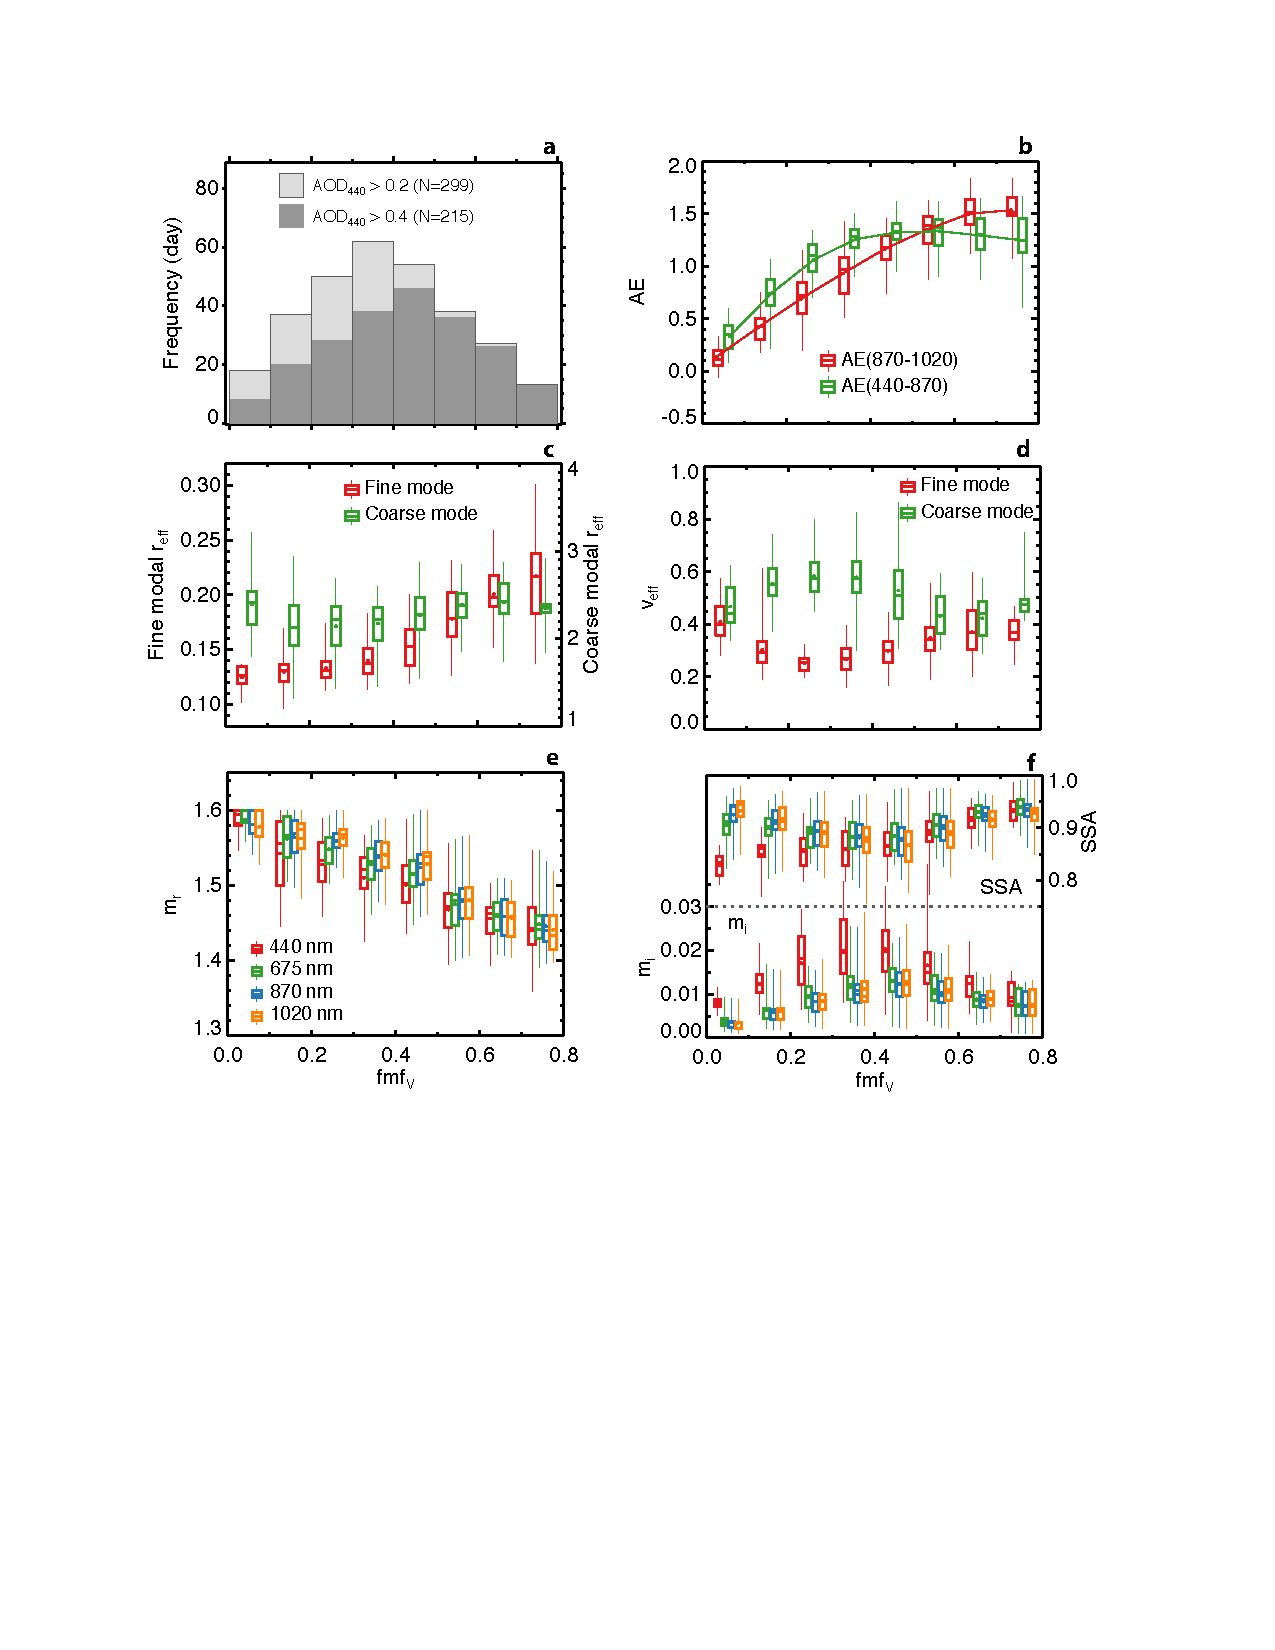
\includegraphics[width={\textwidth}]{figures/inv01.pdf}
  \caption{Climatology of aerosol properties over the Beijing\_RADI site derived
from AERONET daily inversion products during 2011--2013. The variables are shown
as functions of the fine-mode-fraction in terms of the aerosol volume, or
$\fmfv$. Eight bins are applied for $\fmfv$ from 0 to 0.8 with an increment of 0.1.
The six panels are: (a) Histogram of used data; (b) the Ångström exponents (AE)
derived from from 870 to 1020 nm (red) and from 440 to 870 nm (green)
wavelength pairs; (c) the effective radius for aerosols in the fine (red) and
coarse (green) mode; (d) the effective variance in the fine (red) and coarse
(green) mode (green); (e) the real part of the refractive index at 440, 675,
870, and 1020 nm; and (f) the imaginary part of the refractive index and
aerosol SSA at the same wavelengths.}
  \label{fig:invap}
\end{figure}

%% Selected case
\begin{table}[b]
  \centering
  \small
  \caption{Main characteristics of case studies in this work.}
  \label{tab:invcase}
  \begin{tabular}{p{2em} C{7em}  C{4em} C{2em} C{5em} C{4em} C{4em} C{2em}}
  \toprule
  Case  & Date \& Time \newline UTC& $\theta_0(^\circ)$ & ${\taua}_{440}$ &
  AE\newline(870/1020nm)& OMI \ce{NO2} \newline(molec/cm$^2$) & 
  OMI \ce{O3} \newline (DU) & Vapor \newline (cm) \\
  \midrule
   A & 02/22/2011 04:30	& 50.3--50.6 & 3.46 & 1.57 & 6.3$\times$10$^{16}$ & 356.5 & 0.86\\
   B & 03/17/2013 03:25 & 43.0--42.2 & 2.74 & 1.39 & 4.2$\times$10$^{16}$ & 332.7 & 0.76\\
   C & 03/22/2013 07:23 & 57.0--60.0 & 1.05 & 1.01 & 4.1$\times$10$^{16}$ & 386.7 & 1.01\\
  \bottomrule
  \end{tabular}
\end{table}

The \textit{a priori} knowledgeis characterized 
with the climatology of aerosol properties
derived from the version 2.0 AERONET daily inversion products of the same site
during 2011--2013. The PSD parameters were analyzed with 299 available daily
inversions when the 440-nm AOD is larger than 0.2. The refractive index and SSA
were analyzed with 215 inversions when the 440-nm AOD is larger than 0.4. In
Figure \ref{fig:invap}, the variables are shown as functions of the 
fine-mode-fraction in terms of the aerosol volume, or $\fmfv$. It can be found 
that the $\fmfv$ from 0.2 to 0.6 accounts for $\sim$70\% of occurrences (Figure
\ref{fig:invap}a), indicating aerosol over this site is dominated by the mixed 
fine-coarse aerosols. The AE derived from the 1020-nm and 870-nm AOD pairs is 
more linearly related to the $\fmfv$ than the 440-nm and 870-nm AE (Figure
\ref{fig:invap}b), because AE over the longer-wavelength pairs is more
sensitive to the component fraction and less sensitive to the change of
component particle size \citep{Schuster06}. From Figure \ref{fig:invap}c--f, 
we determine the \textit{a priori} state ($\xabf$) based on the corresponding mean values. 
For refractive index, we pick their mean values when $\fmfv<0.2$ for the coarse
mode and when $\fmfv>0.6$ for the fine mode. The \textit{a priori} error 
($\epsilon\uda$) for each parameter is determined by the relevant physical 
range, and is listed in the last column of Table \ref{tab:inverr}. 
In addition, we found in the Figure \ref{fig:invap}e that the $\mreal$ 
retrievals decrease quasi-linearly with the increasing $\fmfv$, which indicates
the $\mreal$ has distinct values between aerosols in the fine and the coarse
modes over this site. It is expected that the $\mreal$ in the mixed aerosol
situations, e.g., $0.3<\fmfv<0.6$, is also expected to have the separated 
values for fine- and coarse-mode particles.

With the above \textit{a priori} characterization, we performed retrievals for three
cases, respectively, on 22 February 2011, 17 March 2013, and 22 March 2013
(hereinafter, cases A, B, and C). A brief characterization of these cases is
presented in Table \ref{tab:invcase}. Indeed, these cases represent different 
aerosol mixtures (according to their AE values): (A) dominated by 
fine particles, (B) well-mixed, and (C) dominated by large particles. 
Moreover, the present algorithm is designed to run with two inversion 
scenarios: the first includes DOLP, while the second ignores
it---hereafter, we label these scenarios type P and I, respectively. An
examination of the difference in the fitting results between these two types of
inversion would indicate the value of DOLP in improving the retrieval. For all
cases, optimal solutions are achieved within less than thirty iterations, and
further iterations yield negligible reduction of the cost function. 

\section{Fitting Residuals} \label{sec:invfit}

The fitting residual characterizes the disagreement between the model and the
measurement. The individual sky radiance residual is defined as a relative
quantity: 
\begin{equation}
e_\text{I}=(I_\text{calc}-I_\text{meas})/I_\text{meas}
\end{equation}
where $I_\text{calc}$ and $I_\text{meas}$ denote the calculated (using the 
retrieved aerosol parameters) and measured sky radiances, respectively. 
In contrast, the fitting residuals for AOD and DOLP are defined by: 
\begin{align}
e_\text{AOD} &= \text{AOD}_\text{calc}-\text{AOD}_\text{meas}, \\
e_\text{DOLP} &= \text{DOLP}_\text{calc}-\text{DOLP}_\text{meas}.
\end{align}
The residual errors for AOD, sky radiance, and DLOP are mean values of
$|e_\text{I}|$, $|e_\text{AOD}|$, and $|e_\text{DOLP}|$, respectively.

%% Figure of Fitting residual
\begin{figure}[t]
  \centering
  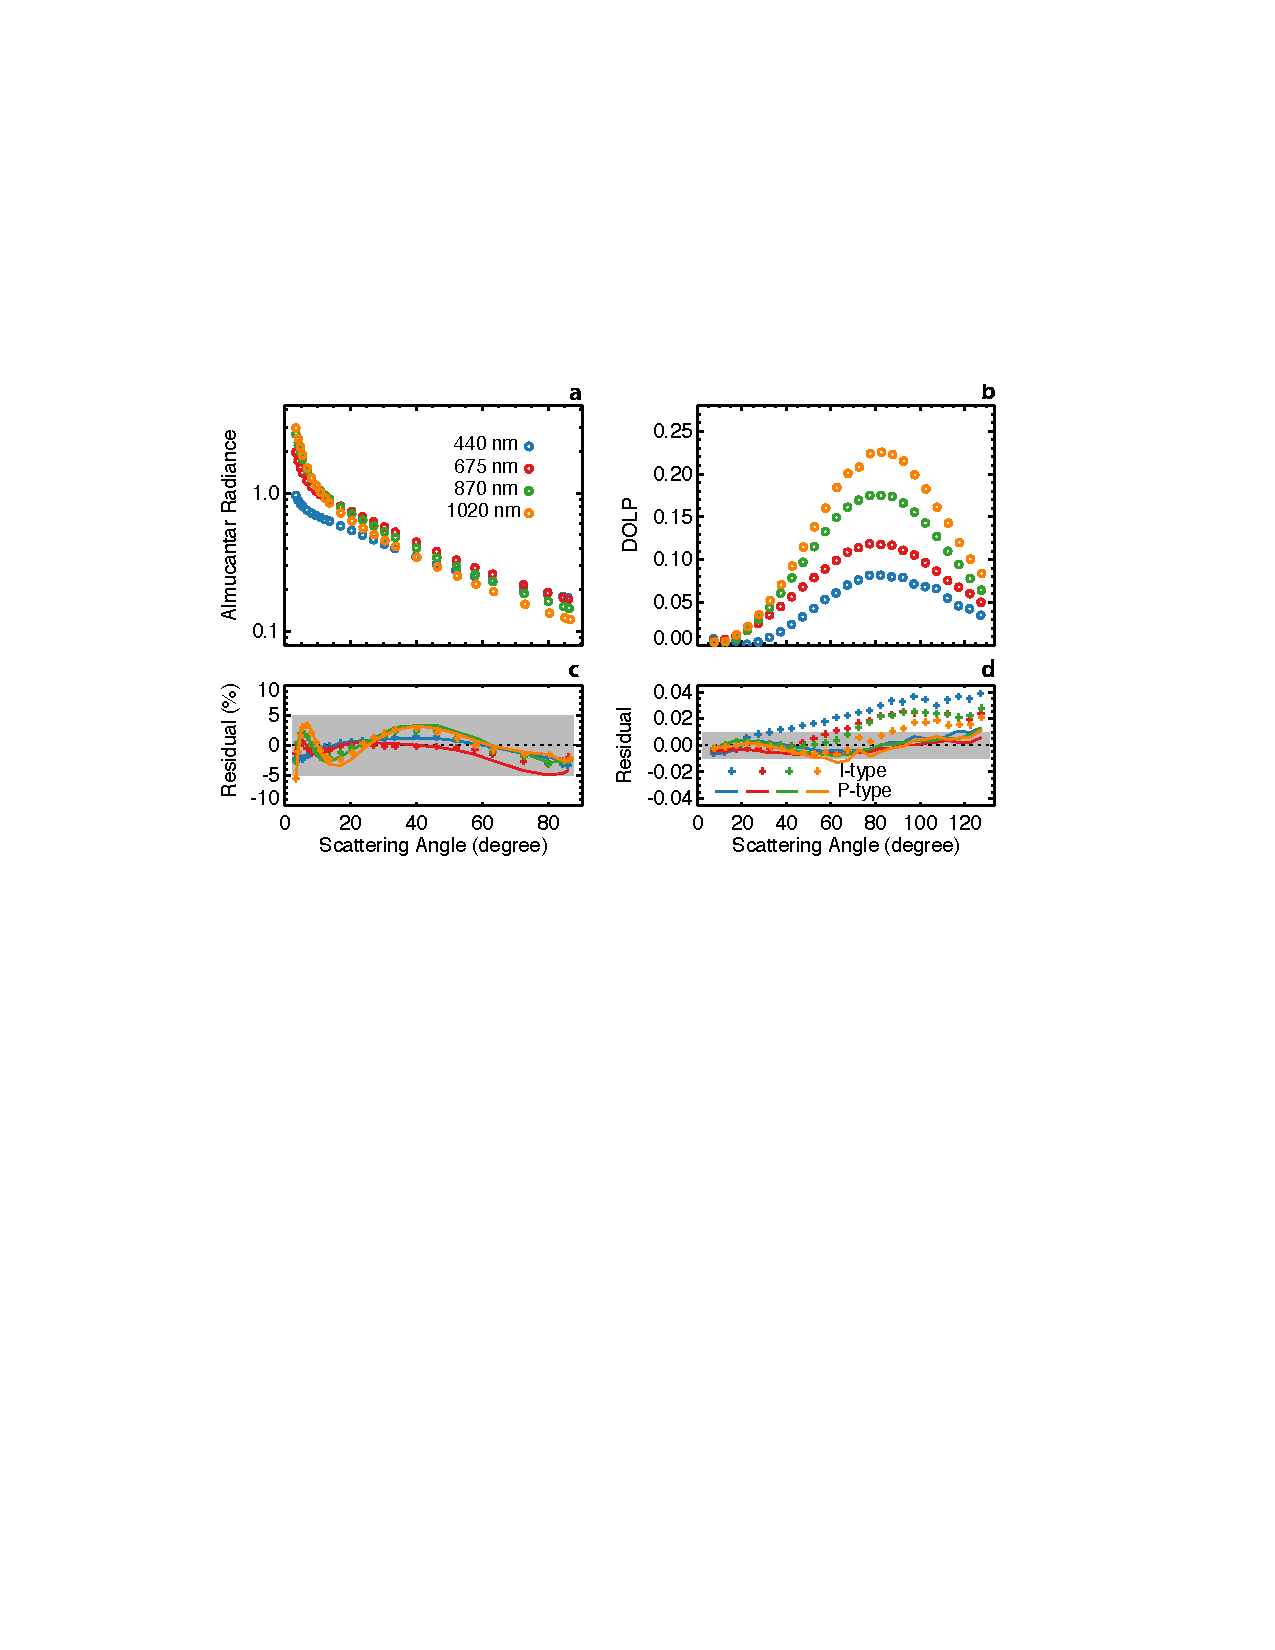
\includegraphics[width={\textwidth}]{figures/inv02.pdf}
  \caption{(a) Measured almucantar normalized radiances. (b) Measured DOLP in
the solar principal plane. (c) Fitting residuals for almucantar radiances by
the P-type inversion (solid curves) and I-type inversion (crosses). (d) Same as
panel (c), but for fitting the residuals of principal-plane DOLP. Four colors
indicate different wavelengths: blue for 440 nm, green for 675 nm, red for 870
nm, and orange for 1020 nm. Gray areas in panels c–d indicate the measurement
uncertainty.}
  \label{fig:invfit}
\end{figure}

Because similar fitting results are found for these three aerosol types
(cases), we illustrate in Figure \ref{fig:invfit} the fitting results for sky 
radiances and DOLP only for the case B. The statistical residual errors are 
displayed in Table \ref{tab:invfit} for all three cases. We found that 
retrievals from both types of inversion can well reproduce these AERONET 
measurements of AOD and sky radiances. Fitting residuals from both types of 
inversions for individual ALM radiance measurement lie within the experimental
uncertainty of 5\%, although the fit of radiances from the P-type inversion 
is slightly deteriorated: residual error is 1.67\% for the P-type compared
1.43\% for the I-type inversion. However, the DOLP residual
error can be much larger for the I-type inversion than that for the P-type
inversion: 0.014 versus 0.004. As these fitting results show, without the
constraints imposed by polarization, the retrieved aerosol microphysical
parameters could result in larger error in polarization simulations,
highlighting the necessity to include polarization in the inversion as an
additional source of constraint. 

%% Fitting residuals
\begin{table}[t]
  \centering
  \small
  \caption{Summary of measurement fitting errors.}
  \label{tab:invfit}
  \begin{tabular}{p{3em} C{6em}  C{6em} C{6em} C{6em}}
  \toprule
  Case &  Inversion type & AOD \newline residual error & 
    Radiance \newline residual error & DOLP \newline residual error \\
  \midrule
   A & I & 0.0005 & 1.68\% & 0.008 \\
     & P & 0.0010 & 1.78\% & 0.005 \\
   B & I & 0.0003 & 1.43\% & 0.014 \\
     & P & 0.0003 & 1.67\% & 0.004 \\
   C & I & 0.0007 & 2.77\% & 0.027 \\
     & P & 0.0034 & 3.73\% & 0.009 \\
  \bottomrule
  \end{tabular}
\end{table}

\section{Retrieved Aerosol Properties} \label{sec:inv0}

Figure \ref{fig:inv01} displays our retrievals from both I-type and P-type 
inversions for the aerosol volume PSD and complex refractive indices. 
Also shown are the retrievals from the AERONET \Dub inversion. 
Table \ref{tab:invpsd} presents the values of the (P-type inversion) retrieved
PSD parameters including $V_0$, $\reff$, $\veff$, $\rv$, and $\sg$ for both 
fine and coarse modes, and corresponding values from the \Dub inversion. 
The PSD in these cases consists of separated fine and coarse aerosol modes. 
In the cases dominated by fine-mode aerosol (A) and
well-mixed aerosol (B), our retrievals agree with the AERONET inversions,
though marginal differences are found in the effective radius and standard
deviation. In case C dominated by coarse-mode aerosols, our algorithm results
in a smaller coarse mode $\reff$ than that from the AERONET algorithm; this may
be caused by our assumption of spherical particles, whereas the \Dub
algorithm considers non-sphericity for coarse particles. We did not find
significant differences in the aerosol volumes between our algorithm and the
\Dub algorithm. As Figure \ref{fig:inv01}b--c indicate, fine-mode volume 
retrieved by the P-type inversion is lower than that retrieved by the 
I-type inversion; such an overestimation from radiance-only inversion was 
also found by \citet{Li09}.

%% Figure retrieval of PSD, refractinve index
\begin{figure}[t]
  \centering
  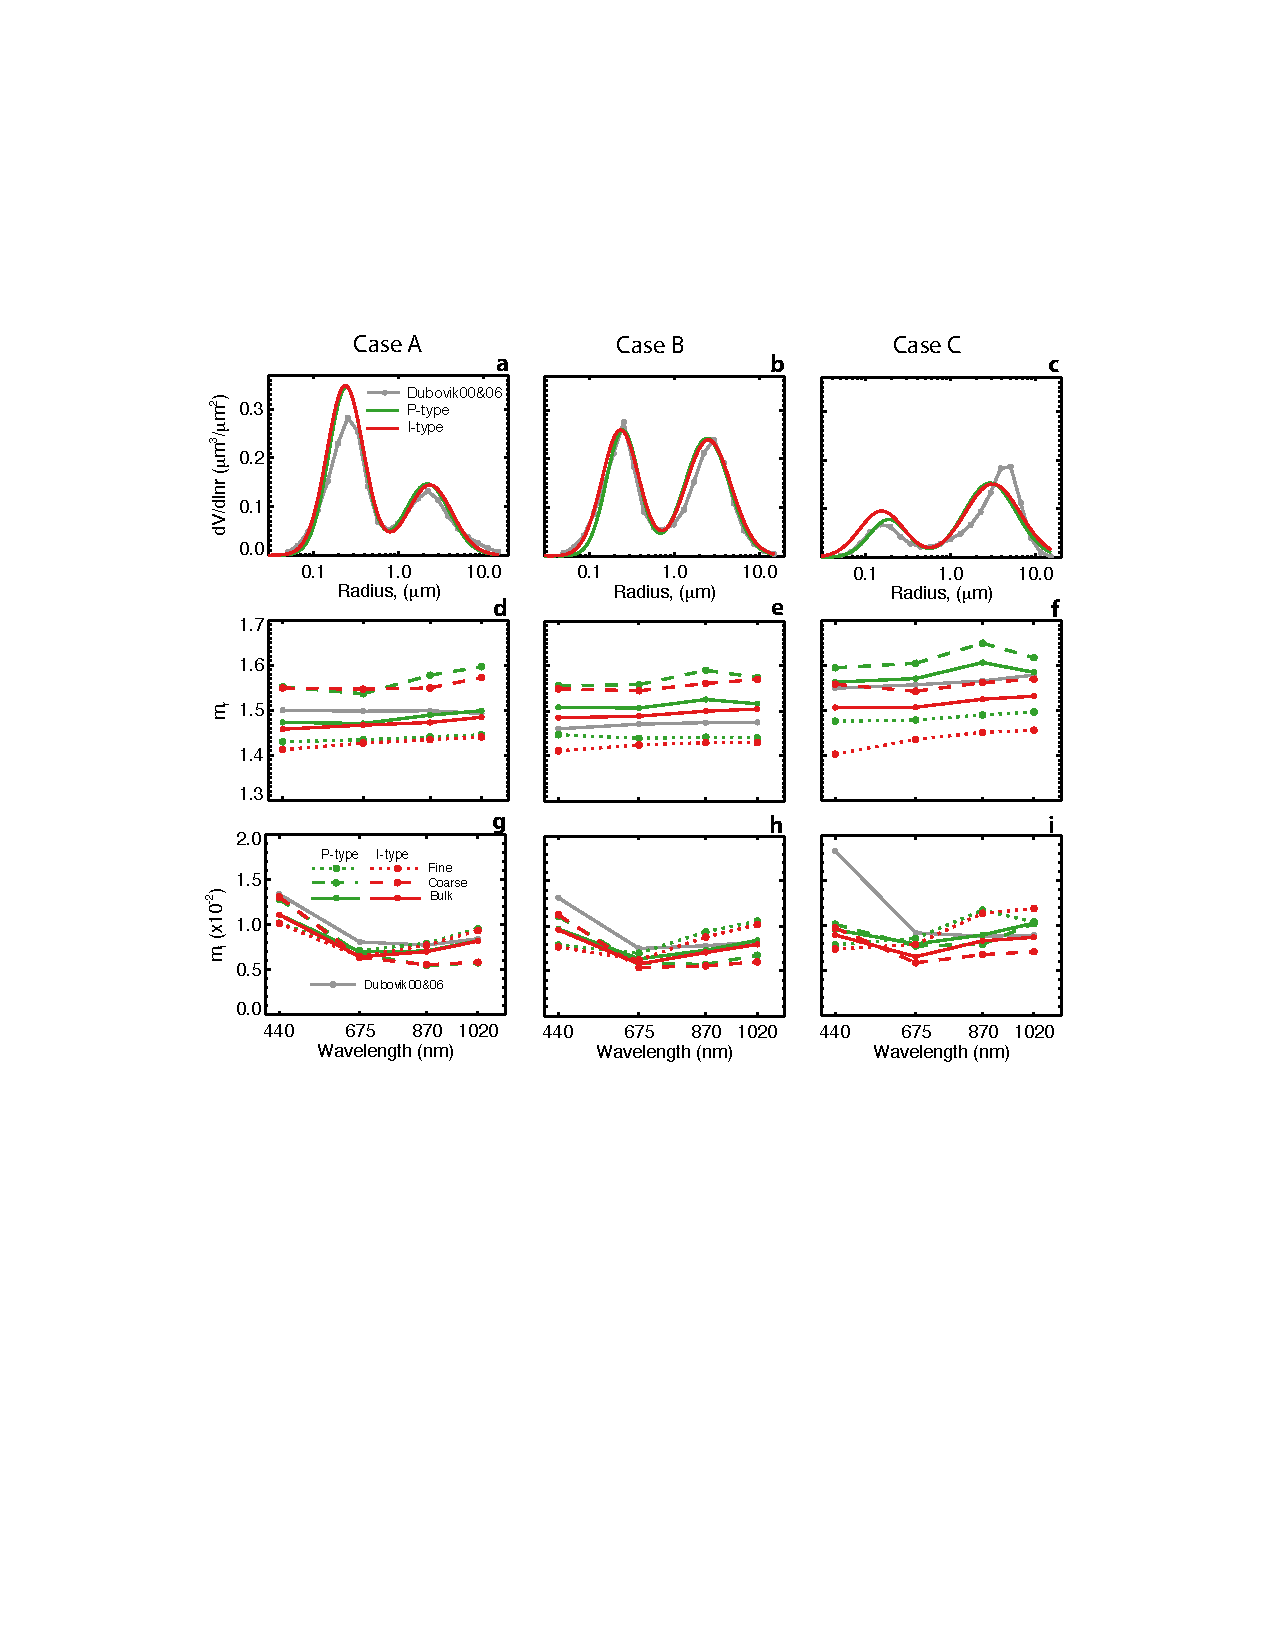
\includegraphics[width={\textwidth}]{figures/inv03.pdf}
  \caption{Retrieved aerosol volume size distribution (PSD) and refractive
index compared with \Dub inversions (gray). P-type and I-type
inversions are represented by green and red colors, respectively. In panels
d--i, the retrievals are shown for aerosols in both fine (dotted) and coarse
(dashed) modes, as well as bulk averages (solid). The PSD relevant quantities
for panels a--c are summarized in Table \ref{tab:invpsd}.}
  \label{fig:inv01}
\end{figure}

%% Figure retrieval of SSA and asy
\begin{figure}[t]
  \centering
  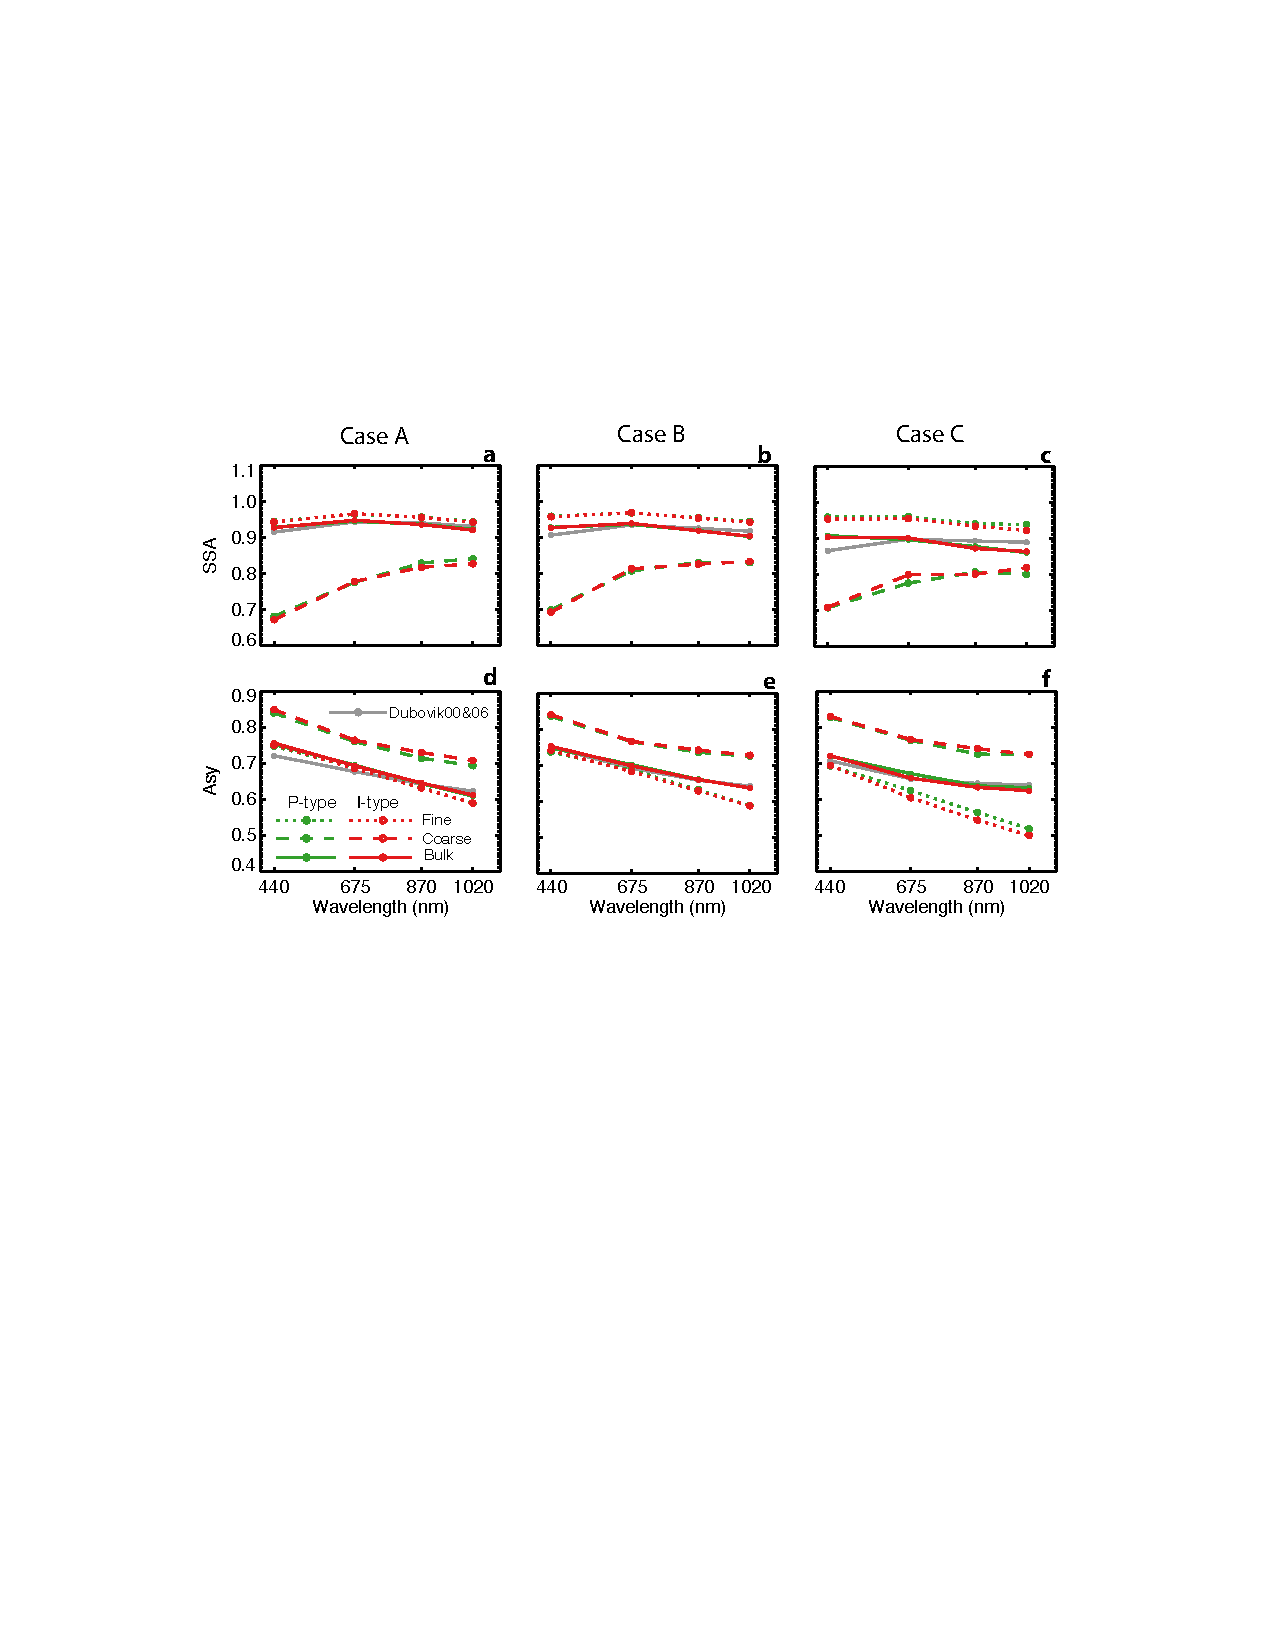
\includegraphics[width={\textwidth}]{figures/inv04.pdf}
  \caption{Same as Figure \ref{fig:inv01}, but for derived aerosol SSA and Asy.}
  \label{fig:inv02}
\end{figure}

In contrast with the \Dub algorithm, which retrieves a single
refractive index for each spectrum that is independent of aerosol size, our
retrieved aerosol refractive indices pertain to the corresponding fine and
coarse modes. In order to get a general impression of the agreement between our
retrievals and the AERONET inversions, we compute the bulk refractive index
that is a weighted average by the particle volume of each mode in our retrieval
\citep[e.g.,][]{Wang07}. According to Figure \ref{fig:inv01}d--f, while the 
bulk value of $\mreal$ is in good agreement (differences $<$ 0.03) with that of
the \Dub retrievals, our retrieval allows for a mode-resolved characterization
 of aerosol refractive index. For instance, the aerosol $\mreal$ has values 
1.5--1.6 in the coarse mode, which is larger than that in the fine mode (1.4--1.5).
In addition, we found that the P-type inversion usually yields higher values of
$\mreal$ compared to the I-type inversion; this finding agrees with \citet{Li09}
in that the radiance-only inversion underestimates $\mreal$. 

%% Table of retrieval results
\begin{table}[t]
  \centering
  \small
  \caption{PSD-related parameters (as illustrated in Figure
\ref{fig:inv01}) retrieved by our P-type inversion, compared
with values from the AERONET \Dub inversion.}
  \label{tab:invpsd}
  \begin{tabular}{p{2em} C{4em} R{4em} R{4em} R{4em} R{4em} R{4em} R{4em}}
  \toprule
  & & \multicolumn{2}{c}{Case A} &
      \multicolumn{2}{c}{Case B} & 
      \multicolumn{2}{c}{Case C} \\
  \cmidrule(r){3-8}
  $\xbf$ &  Units & P-type & AERONET & P-type & AERONET & P-type & AERONET \\
  \midrule
  $V_0\fine$     & $\vunit$ & 0.41  & 0.36  & 0.29  & 0.31  & 0.10  & 0.09  \\
  $\reff\fine$   & $\runit$ & 0.218 & 0.208 & 0.226 & 0.201 & 0.163 & 0.156 \\
  $\veff\fine$   &  --      & 0.25  & 0.32  & 0.22  & 0.32  & 0.31  & 0.33  \\
  $\rv\fine$     & $\runit$ & 0.243 & 0.240 & 0.249 & 0.232 & 0.186 & 0.179 \\
  $\sg\fine$     &  --      & 1.60  & 1.69  & 1.56  & 1.69  & 1.68  & 1.70  \\
  \hline
  $V_0\coarse$   & $\vunit$ & 0.22 & 0.21 & 0.37 & 0.32 & 0.27 & 0.26 \\
  $\reff\coarse$ & $\runit$ & 1.83 & 2.01 & 2.02 & 2.26 & 2.26 & 2.61 \\
  $\veff\coarse$ & --       & 0.44 & 0.53 & 0.45 & 0.38 & 0.65 & 0.50 \\
  $\rv\coarse$   & $\runit$ & 2.20 & 2.44 & 2.44 & 2.65 & 2.91 & 3.28 \\
  $\sg\coarse$   & --       & 1.83 & 1.92 & 1.84 & 1.76 & 2.03 & 1.89 \\
  \bottomrule
  \end{tabular}
\end{table}

According to Figure \ref{fig:inv01}g-–i, the bulk $\mimag$ retrieved by our
algorithm is consistent overall with that from the \Dub algorithm, with both 
retrievals showing similar spectral dependencies. One exception is for case C;
$\mimag$ at 440 nm is about 0.01 from our algorithm but is about 0.02 with the
\Dub algorithm. As expected, our inversion algorithm also offers mode-resolved
$\mimag$. We notice in our retrieval that $\mimag$ shows an increasing 
dependence on the spectral wavelength for the fine mode but a decreasing 
tendency for the coarse mode. 

In the forward modeling framework, the aerosol macrophysical optical properties
act as intermediate model parameters to link the aerosol microphysical
characteristics to the radiation fields. These macrophysical optical parameters
include but are not limited to the aerosol SSA ($\assa$), the scattering phase
function, and the asymmetry factor (Asy). These quantities do not appear in the
state vector; instead, they can be derived from the retrieved microphysical
parameters, and are thus called derived or intermediate parameters. In Figure
\ref{fig:inv02}, we present $\assa$ and Asy from our retrieval, and the 
comparison with their counterparts from the \Dub inversion. In our retrieval,
bulk values of $\assa$ and Asy are again calculated by a scatter-weight 
averaging of the fine and coarse mode values. We found that the bulk $\assa$ 
and Asy from our algorithm and the \Dub algorithm agree very well. 
However, our retrieved coarse-mode $\assa$ varies from 0.7 to 0.9, increasing
with wavelength. In contrast, the retrieved fine-mode $\assa$ runs close to 0.9. 

\section{Improvement over Radiance-Only Retrievals} \label{sec:inv1}

The above comparisons of retrieval results confirm that both P- and I-type
inversions by our algorithm can generate solutions quite consistent with the
current \Dub algorithm. In order to demonstrate the improvements in the
retrieval by including polarization, we compare the retrieval errors between
the P-type and I-type inversions in Table \ref{tab:inverr} for individual aerosol parameters.
Also compared are the errors in the derived $\assa$ and Asy. Clearly, the P-type
inversion yields lower retrieval errors for all the retrieved and derived
parameters; this is confirmed by the theoretical analysis in Chapter
\ref{ch:info} of this thesis. The key points from the comparison are:

(i) Polarization measurements provide important constraints in improving the
retrieval of $V_0$, $\reff$, and $\veff$ for both fine and coarse aerosol modes. For
these three cases, the errors in the retrieved $V_0$ with polarization are less
than 3\% for the fine mode and less than 5\% for the coarse mode, representing a
significant decrease from their counterparts ($\sim$15\% and $\sim$10\%) in the I-type
inversion. Adding polarization can also decrease the error in $\reff$ of both
fine and coarse modes from 10--15\% for the I-type inversion to 3\% and below.
Errors in $\veff$ retrieved by the P-type inversion are 9--11\% for aerosol in the
fine mode and 17--26\% in the coarse mode, whereas they can exceed 60\% with the
I-type inversion.

(ii) Polarization measurements also provide useful constraints in improving the
refractive index retrievals. The most significant improvement is found in the
fine-mode $\mreal$, where the error is lower than 0.01 for the P-type inversion,
compared to 0.02--0.04 for the I-type inversion. The error in the coarse-mode
$\mreal$ from P-type inversion ranges from 0.04 to 0.11, depending on the prevalence
of coarse-mode particles. For retrieving $\mimag$, the inclusion of polarization
reduces the error by 10--30\%, a value also depending on coarse-mode dominance. 

(iii) Adding the polarization yields better estimates of the aerosol SSA and
Asy for both aerosol modes. From P-type inversion, the errors in the retrieved
$\assa$ are lower than 0.02 for aerosols in the fine mode and 0.06 for aerosols in
the coarse mode, representing a 10--40\% decrease from the I-type inversion. As
expected, errors in the Asy also reveal a 30--50\% decrease. 

%% Table of retrieval error
\begin{table}[t]
  \centering
  \small
  \caption{Errors on the retrieved and derived parameters from both types of
inversion\textsuperscript{a}.}
  \label{tab:inverr}
  \begin{tabular}{p{2em} R{4em} R{3em} R{4em} R{3em} R{4em} R{3em} R{4em}}
  \toprule
  & \multicolumn{2}{r}{Case A} &
    \multicolumn{2}{r}{Case B} &
    \multicolumn{2}{r}{Case C} \\
  \cmidrule(r){2-7}
  $\xbf$ & $\errp$ & $\erri$ & $\errp$ & $\erri$ & $\errp$ & $\erri$ & $\epsilon\uda$ \\
  \midrule
  $V_0\fine$     & 2.1\%&15\%&2.2\%&18\%&3.0\%&25\%&100\%\\
  $\reff\fine$   & 1.3\%&9.2\%&1.3\%&11\%&2.4\%&14\%&80\%\\
  $\veff\fine$   & 9.3\%&33\%&9.3\%&38\%&11\%&33\%&80\%\\
  $\mreal\fine$  & 0.005&0.020&0.006&0.023&0.009&0.035&0.14\\
  $\mimag\fine$  & 0.002&0.002&0.003&0.004&0.004&0.006&0.010\\
  $\assa\fine$   & 0.009&0.010&0.016&0.018&0.021&0.037&--\\
  Asy$\fine$     & 0.003&0.005&0.003&0.006&0.003&0.009&--\\
  \hline
  $V_0\coarse$   & 4.8\%&14\%&3.2\%&10\%&2.9\%&9.4\%&100\%\\
  $\reff\coarse$ & 6.7\%&15\%&3.3\%&7.1\%&1.9\%&6.0\%&80\%\\
  $\veff\coarse$ & 26\%& 66\%&17\%&48\%&10\%&33\%&80\%\\
  $\mreal\coarse$& 0.108&0.137&0.080&0.122&0.044&0.100&0.16\\
  $\mimag\coarse$& 0.006&0.007&0.005&0.006&0.003&0.005&0.008\\
  $\assa\coarse$ & 0.059&0.065&0.050&0.058&0.031&0.051&--\\
  Asy$\coarse$   & 0.024&0.036&0.018&0.028&0.012&0.025&--\\
  \bottomrule
  \multicolumn{8}{p{32em}}{\textsuperscript{a}$\errp$ and $\erri$ are retrieval error 
respectively from the P-type and I-type inversions, $\epsilon\uda$ is the a priori error.}
  \end{tabular}
\end{table}

\section{Summary}

In this chapter, we applied the new algorithm to a suite of photo-polarimetric
measurements taken from the new-generation SunPhotometer at the Beijing\_RADI
AERONET station. In order to demonstrate the importance of adding polarization
measurements, we performed aerosol retrievals from radiance measurements only
(the I-type inversion), in addition to the retrievals using both radiance and
polarization measurements (the P-type inversion). We found that, for both types
of inversion, the fitting errors for the AOD and sky radiance are much smaller
than the calibration uncertainties (0.02 for AOD and 5\% for sky radiance).
Also, the fitting errors of the degree of linear polarization (DOLP) with the
P-type inversion are much smaller than the calibration error ($\sim$0.01). However,
the DOLP fitting errors in the I-type inversion usually exceed 0.01, and even
reach 0.04 for many individual measurements in the case dominated by coarse
aerosols, which highlights the necessity to include polarization in the
inversion as an additional source of constraint.

Our retrieval results are generally consistent with the AERONET inversion
products, but we found distinct differences between the values of the
refractive index and SSA for the fire- and coarse-mode aerosols. For these
three cases selected for our study, we found that the retrieved real part
refractive index is about 1.5--1.6 in the coarse mode, which is higher than
those for the fine mode, 1.4--1.5. Also, the coarse-mode aerosols are more
absorbing than the fine-mode ones.

We also compared the retrieval error for each retrieved parameters between the
I-type and P-type inversions. A comparison analysis indicates that the
retrieval error can be reduced by at least 50\% in PSD parameters, by 10–30% in
the refractive index components, and by 10--40\% in the aerosol SSA. These error
reductions depend on the fine/coarse-mode fraction, specifics of
instrumentation, and aerosol properties. These improvements in the P-type
inversion are consistent with the theoretical analysis in Chapter \ref{ch:info}
of this thesis.

The promising results in this study are obtained from the initial development
and preliminary applications of a new algorithm targeted for the retrieval of
aerosol properties from new-generation AERONET measurements. Future
developments will include, but not be limited to, the treatment of
non-spherical large aerosol particles like mineral dust, and the consideration
of tri-modal aerosols for special situations. While the bi-lognormal PSD can
well represent the aerosol size spectrum in most cases, future research efforts 
will include the implementation of tri-modal aerosol mixtures in situations of
cloud formation \citep{Eck12} or volcanic aerosols \citep{Eck10}.
Moreover, extensive retrievals for a longer period of time will also be
performed over sites where CE318-DP SunPhotometer instruments have been
installed (i.e., Beijing\_RADI and Lille).

\section{Acknowledgements}

We thank Li Li for providing the AERONET radiance and polarization
measurements over Beijing\_RADI site. We acknowledge the computational
support from the Holland Computing Center at Unversity of Nebraska.
This work is supported by a NASA Earth and Space Science
Fellowship and the NASA Radiation Sciences Program and the Glory mission
program. This chapter has been published as an article on
\textit{Journal of Geophysical Research – Atmospheres} \citep{Xu15b}.
 

%% backmatter is needed at the end of the main body of your thesis to
%% set up page numbering correctly for the remainder of the thesis
\backmatter

%% Start the correct formatting for the appendices
\appendix

\chapter{Abbreviations and Acronyms}
\chapter{Symbols}

%% Bibliography goes here (You better have one)
%% BibTeX is your friend
\begin{onehalfspacing}
\bibliographystyle{agu08}
\bibliography{phdthesis}
\end{onehalfspacing}
%% Pull in all the entries in the bibtex file. Is is a useful trick to
%% check all your references.
%\nocite{*}

\newpage
\begin{listofpub}
  List my publication here
\end{listofpub}

%% Index go here (if you have one)

\end{document}
\endinput
%%
%% End of file `thesis-test.tex'.
